\documentclass{article}
\usepackage[brazil]{babel}
\usepackage[T1]{fontenc} % Encoding da fonte
\usepackage[utf8]{inputenc} % Encoding da entrada de dados
\usepackage{amsmath} % Comandos matemáticos
\usepackage{amssymb} % Símbolos matemáticos
\usepackage{graphicx} % Permite inclusão de fotos
\usepackage{mathrsfs} % Permite uso da fonte 'Ralph Smith's Formal Script'
\usepackage{hhtensor} % Notação de vetores (seta em cima)
\usepackage[pt-BR]{datetime2} % Para colocar a data apenas com o mês
\usepackage{indentfirst} % Identa os primeiros parágrafos de uma seção
\usepackage[top=3cm,bottom=2cm]{geometry} % Seta as margens do documento
\usepackage{ragged2e} % Ambientes de alinhamento
\usepackage{multicol} % Multi-colunas
\usepackage[american,cute inductors,nooldvoltagedirection]{circuitikz} %circuitikz, desenho de circuitos
\usepackage{enumitem} % Setar identação nos itemizes
\setlist[itemize]{leftmargin=*}

\usetikzlibrary{matrix,decorations.pathreplacing,calc,arrows,decorations.markings,shapes.misc,external}
\ctikzset{label/align= straight,diodes/scale=0.7}
\tikzexternalize[prefix=tikz/, figure name = ckt\thesubsubsection-]
\numberwithin{equation}{section}
\newlength\Colsep
\setlength\Colsep{10pt}
\newcommand{\curtovirtual}{($(opamp.+)+(0.3,0)$) to[open,v^=$ $, l=0, voltage shift=1] ($(opamp.-)+(0.3,0)$)}
\newcommand{\deo}[1]{\dfrac{d^{#1}e_o}{dt^{#1}}}
\newcommand{\dei}[1]{\dfrac{d^{#1}e_i}{dt^{#1}}}
\let\l\left
\let\r\right
\let\dfr\dfrac
\newcommand{\itembull}[1]{\noindent\textbf{\small{\textbullet \hspace{1.5mm}#1}}}

\title{\begin{center}
    
\includegraphics[width=0.45\textwidth]{img/ceeca.png}
\end{center}
\vspace{2mm}
\textbf{Circuitos Elétricos I}}
\author{Colaboradores: Joe Ferreira Scholtz e Pedro Rodrigues de Lima}
\date{\today}

\begin{document}

\maketitle

\newpage
\tableofcontents
\newpage

\section{Prefácio}
\label{sec:pref}

\subsection{Comentários}
\label{subsec:coment}

Este documento tem como objetivo suprir a base teórica necessária para o aprendizado do método de resolução de circuitos elétricos no domínio do tempo (e brevemente em frequência) sob uma abordagem voltada ao uso combinado e simultâneo das Leis de Kirchhoff.

É importante salientar que o presente documento não é, de modo algum, tão completo e/ou matematicamente rigoroso quanto um livro-texto respeitável deve ser, pelo fato de que, dentre outras coisas, o mesmo foi criado em um curto intervalo de tempo e é destinado, principalmente, a auxiliar os alunos das diversas Engenharias, nossos colegas e amigos. Por isso, muitas das deduções matemáticas serão omitidas, bem como alguns fatos/conceitos sobre o funcionamento físico de circuitos elétricos serão considerados verdadeiros, sem maior embasamento experimental ou teórico.

A organização dos tópicos a serem abordados foi escolhida de modo a seguir a ordem lógica de crescente complexidade quanto às suas seções, porém não tanto quanto às suas subseções.

\newpage

\section{Introdução}
\label{sec:introd}

A primeira coisa que é válida a ser salientada sobre circuitos é o fato desses ``diagramas elétricos''  serem intrinsecamente, na verdade, uma modelagem matemática de equações diferenciais.

\subsection{Variáveis Fundamentais}
\label{subsec:variaveis}

\subsubsection{Corrente Elétrica}
\label{subsubsec:corrente}

A mais básica propriedade de sistemas elétricos é a \textbf{carga elétrica}, que representa as concentrações de prótons ($+$) e de elétrons ($-$) em um corpo (um fio condutor, por exemplo). Se uma força eletromotriz for aplicada em dito corpo, a mesma causará uma movimentação das cargas negativas em relação às positivas, definindo um certo fluxo de carga denominado \textbf{corrente elétrica}. Portanto, a corrente elétrica $i$ é o fluxo de carga $q$ por unidade de tempo $t$, isto é

\begin{equation}
    i = \dfrac{dq}{dt},
\end{equation}

\noindent mensurada, no Sistema Internacional de Unidades, em ampères [$A$].

Antes da inclusão dos elétrons nos modelos elétricos, acreditava-se que o fluxo de carga partia do terminal positivo em direção ao negativo, dando origem a uma grandeza ainda utilizada e hoje conhecida como \textbf{corrente convencional}. Este e a grande maioria dos outros materiais de circuitos elétricos adotam a corrente convencional, apesar de que isso apenas implica mudança de sentido do fluxo de cargas. Por isso, quando afirma-se que existe uma corrente de, digamos, $i_1=1A$, está implícito que esta representa a movimentação das cargas positivas. Analogamente, uma corrente $i_2=-1A$ indica movimentação no sentido oposto. Por isso, a mesma corrente pode ser representada de duas maneiras:

\begin{center}
    \begin{tikzpicture}
        \draw
            (0,0) to[short,*-,f=$i$] (2,0)
            (2,0) to[short,-*,f<=$-i$] (4,0)
        ;
    \end{tikzpicture}
\end{center}

Ao resolver um circuito elétrico, pode-se atribuir um sentido arbitrário para as correntes, desde que a atribuição seja seguida integralmente ao longo da resolução. No caso do sentido real da corrente ser oposto ao escolhido, o valor de corrente encontrado deverá ser negativo.

Existem dois principais tipos de corrente. Chama-se de \textbf{corrente contínua} (do inglês, \textit{direct current, DC}) aquela que não varia com o tempo, ou seja, constante. Já uma corrente que varia de forma senoidal, com média zero, é denominada \textbf{corrente alternada} (\textit{alternating current, AC}).

\subsubsection{Tensão}
\label{subsubsec:tensão}

A \textbf{tensão elétrica} $V$ (também denotada por $e$) representa a transferência de energia $E$ envolvida na movimentação das cargas elétricas $q$, isto é

\begin{equation}
    V = \dfrac{dE}{dq},
\end{equation}

\noindent sendo mensurada em volts [$V$].

A tensão é sempre medida entre dois pontos, digamos, $a$ e $b$, e representa a \textbf{diferença de potencial} entre os terminais $a$ e $b$. Por isso, uma tensão $V_{ab}$ sempre pode ser expressa por $V_{ab}=\tilde{V}_a - \tilde{V}_b$, sendo $\tilde{V}_x$ o potencial elétrico no ponto $x$. Os sinais de ($+$) e ($-$) definem a \textbf{polaridade} da tensão, indicando um \textbf{referencial} para sua magnitude. A figura abaixo ilustra a representação da tensão em uma carga genérica.

\begin{center}
    \begin{tikzpicture}
        \draw
            (0,0) node[label={left:$a$}]{} to[european resistor,v=$V_{ab}$,*-*] (3,0) node[label={right:$b$}]{}
            (3,0) to[open,v=$V_{ba}$] (0,0)
        ;
    \end{tikzpicture}
\end{center}

\noindent Note que $V_{ba} = -V_{ab}$. Por isso, é comum omitir o subíndice e apenas utilizar-se da magnitude e da polaridade da tensão. Além disso, na maior parte dos circuitos elétricos, atribui-se que o referencial é tal que possua potencial nulo, conhecido como \textbf{terra} (do inglês, \textit{ground, GND}). Incluindo o terra no modelo genérico e excluindo os subíndices, o circuito é:

\vspace{2mm}

\begin{center}
    \begin{tikzpicture}
        \draw
            (0,0) node[label={left:$a$}]{} to[european resistor,v=$V$,*-] (3,0) node[ground]{}
        ;
    \end{tikzpicture}
\end{center}

\textbf{Observação:} Neste material, o terra será omitido e a referência será o potencial comum das fontes independentes (em geral, na parte inferior do circuito). Além disso, diz-se que a tensão ``cai'' quando é lida do terminal positivo para o negativo. Do contrário, a tensão ``sobe''.

\subsection{Elementos e Relações Volt-Ampère}
\label{subsec:elements}

\subsubsection{Elementos Passivos}
\label{subsubsec:passivos}

Componentes passivos não conseguem, por si só, gerar e/ou manipular sinais. Quando combinados com elementos ativos, no entanto, permitem a implementação de diversos sistemas analógicos. O sentido da corrente nos passivos é sempre dado de modo que o fluxo passe do terminal positivo para o negativo. Alternativamente, a polarização da tensão sempre terá seu terminal positivo definido pelo ponto em que a corrente ``entra''. Alguns exemplos são os resistores, os capacitores, e os indutores.

\begin{center}{\textbf{Resistor}}\end{center}

\center{
\begin{tikzpicture}\draw
	(0, 0) to[R, v=$V_{R}$, f=$i_{R}$,*-*] (2.5, 0)
;\end{tikzpicture}
}
\begin{equation}
    V_{R} = Ri_{R} \hspace{0.2cm}[V]
    \hspace{0.6cm}
    i_{R} = \frac{V_{R}}{R} \hspace{0.2cm} [A]
    \hspace{0.6cm}
    P_{R}\footnote{\label{footnote:potencias} A diferença entre P e Q e suas unidades de medida são devidamente esclarecidas na Seção \ref{subsubsec:unidades}.} = V_{R}i_{R} \hspace{0.2cm} [W]
    \hspace{0.6cm}
    E_{R} = Ri_{R}^{2}t \hspace{0.2cm} [J]
\end{equation}

\vspace{3mm}
\begin{center}{\textbf{Capacitor}}\end{center}
\center{
\begin{tikzpicture}\draw
	(0, 0) to[C, f=$i_{C}$,*-*] (2.5, 0)
	(0, -0.3) to[open, v=$V_{C}$] (2.5, -0.3)

;\end{tikzpicture}
}
\begin{equation}
    V_{C} = \frac{1}{C}\int_{0}^{t}{i_{C}} d\tau \hspace{0.2cm}[V]
    \hspace{0.6cm}
    i_{C} = C \frac{dV_{C}}{dt} \hspace{0.2cm} [A]
    \hspace{0.6cm}
    Q_{C}\footnotemark[1] = V_{C}i_{C} \hspace{0.2cm} [VAr]
    \hspace{0.6cm}
    E_{C} = \frac{1}{2}CV_{C}^{2} [J]
    \end{equation}

\vspace{3mm}
\begin{center}{\textbf{Indutor}}\end{center}
\center{
\begin{tikzpicture}\draw
	(0, 0) to[L, v=$V_{L}$, f=$i_{L}$,*-*] (2.5, 0)
;\end{tikzpicture}
}
\begin{equation}
    V_{L} = L \frac{di_{L}}{dt} \hspace{0.2cm}[V]
    \hspace{0.6cm}
    i_{L} = \frac{1}{L}\int_{0}^{t}{V_{L}} d\tau \hspace{0.2cm} [A]
    \hspace{0.6cm}
    Q_{L}\footnotemark[1] = V_{L}i_{L} \hspace{0.2cm} [VAr]
    \hspace{0.6cm}
    E_{L} = \frac{1}{2}Li_{L}^{2} [J]
\end{equation}

\vfill
\justifying
\subsubsection{Elementos Ativos Independentes}
\label{subsubsec:ativos}

Componentes ativos são capazes de gerar e/ou amplificar sinais elétricos. Alguns exemplos são as fontes e os transistores.

\vspace{3mm}

\begin{minipage}[c][5cm]{\dimexpr0.45\textwidth-0.5\Colsep\relax}
    \begin{center}{\textbf{Fonte de Tensão}}\end{center}

    Gera uma tensão $e_i$ entre seus terminais, enquanto a corrente entre seus terminais é independente e determinada pelo resto do circuito.
    \center{
    \begin{tikzpicture}\draw
        (0, 2) to[V, l=$e_i$,*-*] (0, 0)
    ;\end{tikzpicture}
    }
\end{minipage} \hfill
\begin{minipage}[c][2cm][c]{\dimexpr0.05\textwidth-0.5\Colsep\relax}

\end{minipage} \hfill
\begin{minipage}[c][5cm]{\dimexpr0.45\textwidth-0.5\Colsep\relax}
    \begin{center}{\textbf{Fonte de Corrente}}\end{center}

    Gera uma corrente $i$ entre seus terminais, enquanto a tensão entre seus terminais é independente e determinada pelo resto do circuito.
    \center{
    \begin{tikzpicture}\draw
        (0, 0) to[I,l_=$i_{i}$,*-*] (0, 2)
    ;\end{tikzpicture}
    }
\end{minipage} \hfill
\justifying
\subsubsection{Elementos Controlados}
\label{subsubsec:controlados}
Elementos controlados, também chamados dependentes, dependem de algum outro elemento do circuito.

\begin{center}{\textbf{Fonte Controlada de Tensão}}\end{center}
Gera uma tensão $Kv \hspace{0.25cm}[V]$ ou $Ki$ [$\frac{V}{A}$A] entre seus terminais, sendo $v,i$, respectivamente, a tensão e a corrente em algum outro componente do circuito e $K$, uma constante real, o ganho da fonte.\\
\begin{minipage}[c][4cm]{\dimexpr\textwidth-0.5\Colsep\relax}
    \center{\begin{tikzpicture}\draw
        (1, 2) to[short, -*] (0, 2)
        (1, 2) to[european resistor, v_=$v$] (1, 0)
        (1, 0) to[short, -*] (0, 0)
        (3, 2) to[short, -*] (4, 2)
        (3, 2) to[V, l_=$Kv$] (3, 0)
        (3, 0) to[short, -*] (4, 0)
    ;\end{tikzpicture} \hspace{2cm}
    \begin{tikzpicture}\draw
        (1, 2) to[short, -*, f_<=$i$] (0, 2)
        (1, 2) to[european resistor] (1, 0)
        (1, 0) to[short, -*] (0, 0)
        (3, 2) to[short, -*] (4, 2)
        (3, 2) to[V, l_=$Ki$] (3, 0)
        (3, 0) to[short, -*] (4, 0)
    ;\end{tikzpicture}
    }
\end{minipage}

A tensão e corrente $v,i$ são chamadas, nesse contexto, de ``variáveis de controle''.

\begin{center}{\textbf{Fonte Controlada de Corrente}}\end{center}
Gera uma corrente $Ki \hspace{0.25cm}[A]$ ou $Kv$ \hspace{0.25cm}[$\frac{A}{V}$V] entre seus terminais, sendo $v,i$, respectivamente, a tensão e a corrente em algum outro componente do circuito e $K$, uma constante real, o ganho da fonte. \\
\begin{minipage}[c][4cm]{\dimexpr\textwidth-0.5\Colsep\relax}
    \center{\begin{tikzpicture}\draw
        (1, 2) to[short, -*] (0, 2)
        (1, 2) to[european resistor, v_=$v$] (1, 0)
        (1, 0) to[short, -*] (0, 0)
        (3, 2) to[short, -*] (4, 2)
        (3, 0) to[I, l=$Kv$] (3, 2)
        (3, 0) to[short, -*] (4, 0)
    ;\end{tikzpicture} \hspace{2cm}
    \begin{tikzpicture}\draw
        (1, 2) to[short, -*, f_<=$i$] (0, 2)
        (1, 2) to[european resistor] (1, 0)
        (1, 0) to[short, -*] (0, 0)
        (3, 2) to[short, -*] (4, 2)
        (3, 0) to[I, l_=$Ki$] (3, 2)
        (3, 0) to[short, -*] (4, 0)
    ;\end{tikzpicture}
    }
\end{minipage}

\newpage
\subsubsection{Instrumentos}
\label{subsubsec:instrumentos}
Elementos ideais cuja função é medir algum valor em outro elemento do circuito.

\vspace{-1.6cm}

\noindent\begin{minipage}{\textwidth}
    \begin{minipage}[t][4.5cm]{\dimexpr0.45\textwidth-\Colsep\relax}
        \begin{center}{\textbf{Voltímetro}}\end{center}
        Mede a tensão $V$ entre seus terminais. Idealmente, o voltímetro possui uma impedância infinita\footnotemark, o que implica corrente $0$ (zero) entre seus terminais. Deve ser ligado em paralelo com o componente do qual quer-se medir a tensão.

        \center{
        \begin{tikzpicture}\draw
            (0, 0) to[voltmeter,*-*] (2, 0)
        ;\end{tikzpicture}
        }

    \end{minipage}
    \begin{minipage}[c][4.5cm]{\dimexpr0.05\textwidth-0.5\Colsep\relax}

    \end{minipage} \hfill
    \begin{minipage}[t][4.5cm]{\dimexpr0.45\textwidth-\Colsep\relax}
        \begin{center}{\textbf{Amperímetro}}\end{center}
        Mede a corrente $i$ entre seus terminais. Idealmente, o amperímetro possui uma impedância $0$ (zero), permitindo que a corrente passe livremente (sem resistência) entre seus terminais. Deve ser colocado em série com o componente do qual quer-se medir a corrente.
        \center{
        \begin{tikzpicture}\draw
            (0, 0) to[ammeter,*-*] (2, 0)
        ;\end{tikzpicture}
        }
    \end{minipage} \hfill
\end{minipage}
\footnotetext{Conceitos de Impedância, Paralelo e Série são devidamente definidos na Seção \ref{subsec:def}.}

\subsection{Leis de Kirchhoff}
\label{subsec:Kirchhoff}

As Leis de Kirchhoff são equações formuladas a partir dos conceitos da conservação da energia e da carga em um circuito elétrico. São elas:

\subsubsection{Lei de Kirchhoff das Correntes}
\label{subsubsec:KCL}
\textbf{Definição:} A soma de todas as correntes que entram em um nó é igual à soma de todas as correntes que saem deste mesmo nó. Considera-se um nó, um ponto arbitrário de mesmo potencial (a exemplo de um fio ideal, ou seja, independente do tamanho do fio, não há queda de tensão ao longo de sua extensão) no qual os terminais e, por conseguinte, as correntes de dois ou mais componentes se encontram.
\begin{center}
    $$i_{1}+i_{2}-i_{3} = 0$$
    \begin{tikzpicture}\draw
        (0, 2) to[short, *-, f=$i_{1}$] (2, 2)
        (2, 0) to[short, *-, f=$i_{2}$] (2, 2)
        (4, 2) to[short, *-, f<_=$i_{3}$] (2, 2)
    ;\end{tikzpicture}
\end{center}

\subsubsection{Lei de Kirchhoff das Tensões}
\label{subsubsec:KVL}
\textbf{Definição:} O somatório de tensões em um caminho fechado (malha) é nulo. Alternativamente, pode-se dizer que a soma de todas as tensões que caem (do terminal positivo para o negativo) em uma malha é igual à soma de todas as tensões que sobem (do terminal negativo para o positivo) na mesma malha em uma direção arbitrária. Considera-se uma malha um caminho fechado arbitrário (não necessariamente conectado por um fio, mas fechado no sentido de haver queda de tensão entre cada elemento da malha).
\begin{center}
    $$e_{1}+e_{2}-e_{3}=0$$
    \begin{tikzpicture}\draw
        (0, 0) to[V, l=$e_1$] (0, 3)
        (0, 3) to[V, l=$e_2$,-*] (3, 3)
        (3, 0) to[open, v=$e_3$] (3, 3)
        (0, 0) to[short, -*] (3, 0)
    ;\end{tikzpicture}
\end{center}

\subsection{Outros Conceitos Básicos}
\label{subsec:def}
\subsubsection{Associação em Série}
\label{subsubsec:serie}
Dois componentes são ditos associados em série quando estão conectados de modo que a exata mesma corrente passa por ambos. É possível substituí-los por um componente equivalente sem alterar o valor da corrente, a partir da equivalência entre a soma das tensões dos componentes em série para com a tensão do componente equivalente, resultando nas expressões abaixo.
\begin{itemize}
    \item \textbf{Resistores:} $R_{eq}= R_{1} + R_{2}$\\
    ou, generalizando $R_{eq}= \displaystyle{\sum_{i=1}^{N} R_{i}}$
    \item \textbf{Indutores:} $L_{eq}= L_{1} + L_{2}$\\
    ou, generalizando $L_{eq}= \displaystyle{\sum_{i=1}^{N} L_{i}}$
    \item \textbf{Capacitores:} $C_{eq}= \left(\displaystyle{\frac{1}{C_{1}}} + \displaystyle{\frac{1}{C_{2}}}\right)^{-1}$\\
    ou, generalizando $C_{eq}= \left(\displaystyle{\sum_{i=1}^{N} \frac{1}{C_{i}}}\right)^{-1}$
\end{itemize}

\noindent\begin{minipage}{\textwidth}
\begin{minipage}[c][2cm][c]{\dimexpr0.45\textwidth-0.5\Colsep\relax}
    \begin{center}
        \begin{tikzpicture}\draw
            (0,0) to[R, l=$R_1$,*-,f=$i$] (2,0)
            (2,0) to[R, l=$R_2$,-*] (4,0)
        ;\end{tikzpicture}
    \end{center}
\end{minipage} \hfill
\begin{minipage}[c][2cm][c]{\dimexpr0.1\textwidth-0.5\Colsep\relax}
    $$\iff$$
\end{minipage} \hfill
\begin{minipage}[c][2cm][c]{\dimexpr0.45\textwidth-0.5\Colsep\relax}
    \begin{center}
        \begin{tikzpicture}
        \draw
            (0,0) to[R, l=\mbox{$R_{eq}=R_{1}+R_{2}$ \hspace{8mm}},*-*,f=$i$] (4,0)
        ;\end{tikzpicture}
    \end{center}
\end{minipage}
\end{minipage}


\subsubsection{Associação em Paralelo}
\label{subsubsec:paralelo}
Dois componentes são ditos associados em paralelo quando estão conectados de modo que a exata mesma diferença de potencial (tensão) caia em ambos. Neste caso, é possível substituí-los por um componente equivalente sem alterar o valor da tensão, a partir da igualdade entre a soma das correntes individuais dos componentes em paralelo para com a corrente do componente equivalente (o qual, frisando, possui a mesma tensão), resultando nas expressões abaixo.

\begin{itemize}
    \item \textbf{Resistores:} $R_{eq}= \left(\displaystyle{\frac{1}{R_{1}}} + \displaystyle{\frac{1}{R_{2}}}\right)^{-1}$\\
    ou, generalizando $R_{eq}= \left(\displaystyle{\sum_{i=1}^{N} \frac{1}{R_{i}}}\right)^{-1}$
    \item \textbf{Indutores:} $L_{eq}= \left(\displaystyle{\frac{1}{L_{1}}} + \displaystyle{\frac{1}{L_{2}}}\right)^{-1}$\\
    ou, generalizando $L_{eq}= \left(\displaystyle{\sum_{i=1}^{N} \frac{1}{L_{i}}}\right)^{-1}$
    \item \textbf{Capacitores:} $C_{eq}= C_{1} + C_{2} $\\
    ou, generalizando $C_{eq}= \displaystyle{\sum_{i=1}^{N} C_{i}}$
\end{itemize}

\noindent\begin{minipage}{\textwidth}
\begin{minipage}[c][3cm][c]{\dimexpr0.45\textwidth-0.5\Colsep\relax}
    \begin{center}
        \begin{tikzpicture}\draw
            (0,0) to[R, l=$R_1$,v<=$v$] (0,2)
            (0,2) to[short] (2,2)
            (2,0) to[R, l=$R_2$,v<=$v$] (2,2)
            (0,0) to[short] (2,0)
            (0,0) to[short,-*] (-1,0)
            (2,0) to[short,-*] (3,0)
            (0,2) to[short,-*] (-1,2)
            (2,2) to[short,-*] (3,2)
        ;\end{tikzpicture}
    \end{center}
\end{minipage} \hfill
\begin{minipage}[c][3cm][c]{\dimexpr0.1\textwidth-0.5\Colsep\relax}
    $$\iff$$
\end{minipage} \hfill
\begin{minipage}[c][3cm][c]{\dimexpr0.45\textwidth-0.5\Colsep\relax}
    \begin{center}
        \begin{tikzpicture}\draw
            (0,0) to[R, l=\mbox{$R_{eq}= \left(\displaystyle{\frac{1}{R_{1}}} + \displaystyle{\frac{1}{R_{2}}}\right)^{\displaystyle{-1}}$},v<=$v$] (0,2)
            (0,2) to[short,-*] (1,2)
            (0,0) to[short,-*] (1,0)
            (0,0) to[short,-*] (-1,0)
            (0,2) to[short,-*] (-1,2)
        ;\end{tikzpicture}
    \end{center}
\end{minipage}
\end{minipage}

\subsubsection{Associação de Fontes}
\label{subsubsec:assocfonte}

Analogamente aos componentes passivos, é também possível associar fontes de modo a representar suas contribuições por meio de um único componente.

\vspace{4mm}

\textbf{\small{\textbullet} Fontes de tensão:} Quando em série, pode-se somar as fontes de tensão de acordo com suas polaridades. Segue um exemplo.

\noindent\begin{minipage}{\textwidth}
\centering
\begin{minipage}[c][4cm][c]{\dimexpr0.45\textwidth-0.5\Colsep\relax}
    \begin{center}
        \begin{tikzpicture}
            \draw
            (0,2) to[V_=$e_1$] (0,0)
            (2,2) to[V_=$e_2$] (0,2)
            (2,2) to[V=$e_3$,-*] (4,2)
            (0,0) to[short,-*] (4,0)
            ;
        \end{tikzpicture}
    \end{center}
\end{minipage} \hfill
\begin{minipage}[c][4cm][c]{\dimexpr0.1\textwidth-0.5\Colsep\relax}
    $$\iff$$
\end{minipage} \hfill
\begin{minipage}[c][4cm][c]{\dimexpr0.45\textwidth-0.5\Colsep\relax}
    \begin{center}
        \begin{tikzpicture}
            \draw
            (0,2) to[V_=$e_1+e_2-e_3$] (0,0)
            (0,2) to[short,-*] (2,2)
            (0,0) to[short,-*] (2,0)
            ;
        \end{tikzpicture}
    \end{center}
\end{minipage}
\end{minipage}

\textbf{\small{\textbullet} Fontes de corrente:} Quando em paralelo, pode-se somar as correntes de cada fonte de acordo com seus sentidos. Por exemplo:

\noindent\begin{minipage}{\textwidth}
\centering
\begin{minipage}[c][4cm][c]{\dimexpr0.45\textwidth-0.5\Colsep\relax}
    \begin{center}
        \begin{tikzpicture}
            \draw
            (0,0) to[I,l=$i_1$] (0,2)
            (0,2) -- (2,2)
            (2,0) to[I,l=$i_2$] (2,2)
            (2,2) -- (4,2)
            (4,2) to[I,l=$i_3$] (4,0)
            (4,2) to[short,-*] (5,2)
            (0,0) to[short,-*] (5,0)
            ;
        \end{tikzpicture}
    \end{center}
\end{minipage} \hfill
\begin{minipage}[c][4cm][c]{\dimexpr0.1\textwidth-0.5\Colsep\relax}
    $$\iff$$
\end{minipage} \hfill
\begin{minipage}[c][4cm][c]{\dimexpr0.45\textwidth-0.5\Colsep\relax}
    \begin{center}
        \begin{tikzpicture}
            \draw
            (0,0) to[I,l=$i_1+i_2-i_3$] (0,2)
            (0,2) to[short,-*] (2,2)
            (0,0) to[short,-*] (2,0)
            ;
        \end{tikzpicture}
    \end{center}
\end{minipage}
\end{minipage}

\textbf{Observação:} Não é comum utilizar fontes de tensão em paralelo, muito menos fontes de corrente em série, visto que nessas configurações as fontes impõem seus respectivos valores no circuito. De fato, é impossível que as correntes ou tensões assumam dois valores diferentes em um mesmo ponto. Na prática, conectar duas fontes de forma incorreta pode danificar os componentes e, possivelmente, causar faíscas e explosões. Entretanto, uma aplicação é conectar fontes de tensão idênticas em paralelo, de modo que a corrente e, consequentemente, a potência exigidas de cada fonte são menores. Neste material, considera-se que as fontes são ideais, podendo sempre fornecer a potência requerida pela carga.

\subsubsection{Transformação $\Delta-Y$}
Permite transformar um circuito em configuração $\Delta$ para $Y$ e vice-versa, respeitando às seguintes relações:

\noindent\begin{minipage}{\textwidth}
\begin{minipage}[c][5cm][c]{\dimexpr0.45\textwidth-0.5\Colsep\relax}
    \begin{center}
        \begin{tikzpicture}\draw
            (0,0) to[R,l=$R_a$] (2,3)
            (2,3) to[R,l=$R_b$] (4,0)
            (0,0) to[R,l_=$R_c$] (4,0)
            (0,0) to[short,-*] (-.5,0)
            (2,3) to[short,-*] (2,3.5)
            (4,0) to[short,-*] (4.5,0)
        ;\end{tikzpicture}
    \end{center}
\end{minipage} \hfill
\begin{minipage}[c][5cm][c]{\dimexpr0.1\textwidth-0.5\Colsep\relax}
    $$\iff$$
\end{minipage} \hfill
\begin{minipage}[c][5cm][c]{\dimexpr0.45\textwidth-0.5\Colsep\relax}
    \begin{center}
        \begin{tikzpicture}\draw
            (2,4) to[R,l=$R_{3}$,*-] (2,1.5)
            (0,0) to[R,l=$R_{2}$,*-] (2,1.5)
            (2,1.5) to[R,l=$R_{1}$,-*] (4,0)
        ;\end{tikzpicture}
    \end{center}
\end{minipage}
\end{minipage}

\vspace{1.2cm}

\noindent\begin{minipage}{\textwidth}
\begin{minipage}[c][2cm][c]{\dimexpr0.45\textwidth-0.5\Colsep\relax}
    \begin{center}
    $\Delta \longrightarrow Y$
      \vspace{0.2cm}
     \begin{itemize}
        \item $R_1=\dfrac{R_bR_c}{R_a+R_b+R_c}$
        \item $R_2=\dfrac{R_aR_c}{R_a+R_b+R_c}$
        \item $R_3=\dfrac{R_aR_b}{R_a+R_b+R_c}$
    \end{itemize}

    \end{center}
\end{minipage} \hfill
\begin{minipage}[c][2cm][c]{\dimexpr0.1\textwidth-0.5\Colsep\relax}

\end{minipage} \hfill
\begin{minipage}[c][2cm][c]{\dimexpr0.45\textwidth-0.5\Colsep\relax}
    \begin{center}
    $Y \longrightarrow \Delta$
    \vspace{0.2cm}

    \begin{itemize}
    \item $R_a=\dfrac{R_1R_2+R_2R_3+R_1R_3}{R_1}$
    \item $R_b=\dfrac{R_1R_2+R_2R_3+R_1R_3}{R_2}$
    \item $R_c=\dfrac{R_1R_2+R_2R_3+R_1R_3}{R_3}$
\end{itemize}

    \end{center}
\end{minipage}
\end{minipage}

\vspace{1.5cm}


Vale notar que no caso particular em que todos os resistores são iguais (a $R$, por exemplo), a conversão de $\Delta$ para $Y$ resulta em $R_1=R_2=R_3=\frac{1}{3}R$. No caso da operação inversa, obtém-se $R_a=R_b=R_c=3R$.

As configurações $\Delta$ e $Y$ podem ser rearranjadas em um formato alternativo (o exato mesmo circuito é escrito de maneira ligeiramente diferente). Por isso o nome Transformação $\pi-T$ também é empregado.

\noindent\begin{minipage}{\textwidth}
\begin{minipage}[c][5cm][c]{\dimexpr0.45\textwidth-0.5\Colsep\relax}
    \begin{center}
        \begin{tikzpicture}\draw
            (0,0) to[R,l=$R_a$] (0,3)
            (4,3) to[R,l=$R_b$] (4,0)
            (0,3) to[R,l_=$R_c$] (4,3)
            (0,0) to[short,-*] (-.5,0)
            (0,3) to[short,-*] (-.5,3)
            (4,0) to[short,-*] (4.5,0)
            (4,3) to[short,-*] (4.5,3)
            (0,0) -- (4,0)
        ;\end{tikzpicture}
    \end{center}
\end{minipage} \hfill
\begin{minipage}[c][5cm][c]{\dimexpr0.1\textwidth-0.5\Colsep\relax}
    $$\iff$$
\end{minipage} \hfill
\begin{minipage}[c][5cm][c]{\dimexpr0.45\textwidth-0.5\Colsep\relax}
    \begin{center}
        \begin{tikzpicture}\draw
            (-.5,3) to[R,l=$R_{2}$,*-] (2,3)
            (2,3) to[R,l=$R_{3}$] (2,0)
            (2,3) to[R,l=$R_{1}$,-*] (4.5,3)
            (-.5,0) to[short,*-*] (4.5,0)
        ;\end{tikzpicture}
    \end{center}
\end{minipage}
\end{minipage}


\subsubsection{Linearidade}
A relação entre duas variáveis é dita linear quando respeita a seguinte relação
\begin{itemize}
    \item \textbf{Princípio da Superposição:} $f(a_1 x_{1}+a_2 x_{2})= a_1f(x_{1})+a_2f(x_{2})$, com $a_1$ e $a_2$ constantes.
\end{itemize}
O mais pertinente exemplo é a relação entre tensão e corrente nos circuitos reativos. $v(t)=f(i(t))$ ou $i(t)=f(v(t))$. Alguns exemplos,
    $$v_R(i_R)=Ri_R \implies v_R(i_1+i_2) = R\cdot(i_1+i_2) = Ri_1+Ri_2 = v_R(i_1) + v_R(i_2)$$
    $$v_C(i_C)=\frac{1}{C}\int_0^ti_Cd\tau \implies v_C(i_1+i_2)=\frac{1}{C}\int_0^t(i_1+i_2)d\tau=\frac{1}{C}\int_0^ti_1d\tau+\frac{1}{C}\int_0^ti_2d\tau=v_C(i_1)+v_C(i_2)$$
    $$v_L(i_L)=L\frac{di_L}{dt} \implies v_L(i_1+i_2)=L\frac{d}{dt}(i_1+i_2)=L\frac{di_1}{dt}+L\frac{di_2}{dt}=v_L(i_1)+v_L(i_2)$$

É evidente que o princípio da superposição continua sendo válido para o caso de constantes multiplicando as variáveis $i_1$ e $i_2$.

\subsubsection{Superposição em Circuitos Elétricos}
O Princípio da Superposição possui uma importante aplicação em circuitos elétricos, pois permite que a contribuição de cada fonte seja considerada separadamente, muitas vezes facilitando a resolução de problemas que, de outras formas, levaria a uma solução mais complexa e/ou demorada.

\begin{center}
    \begin{tikzpicture}\draw
        (0,3) to[V,l=$V_1$] (0,0)
        (0,3) to[R,l=$R_1$] (3,3)
        (3,0) to[R,l=$R_2$,v<=$e_0$] (3,3)
        (3,3) to[R,l=$R_3$] (6,3)
        (6,3) to[V,l=$V_2$] (6,0)
        (0,0) -- (6,0)
    ;\end{tikzpicture}
\end{center}

A saída $e_0$ pode ser calculada por superposição, de modo que o problema resume-se a resolver os dois circuitos mais simples abaixo

$$e_0=e_{0_1}+e_{0_2}$$

\noindent\begin{minipage}{\textwidth}
\begin{minipage}[c][5cm][c]{\dimexpr0.5\textwidth-0.5\Colsep\relax}
    \begin{center}
        \begin{tikzpicture}\draw
            (0,3) to[V,l=$V_1$] (0,0)
            (0,3) to[R,l=$R_1$] (3,3)
            (3,0) to[R,l=$R_2$,v<=$e_{0_1}$] (3,3)
            (3,3) to[R,l=$R_3$] (6,3)
            (6,3) -- (6,0)
            (0,0) -- (6,0)
        ;\end{tikzpicture}
    \end{center}
\end{minipage} \hfill
\begin{minipage}[c][5cm][c]{\dimexpr0.5\textwidth-0.5\Colsep\relax}
    \begin{center}
        \begin{tikzpicture}\draw
            (0,3) -- (0,0)
            (0,3) to[R,l=$R_1$] (3,3)
            (3,0) to[R,l=$R_2$,v<=$e_{0_2}$] (3,3)
            (3,3) to[R,l=$R_3$] (6,3)
            (6,3) to[V,l=$V_2$] (6,0)
            (0,0) -- (6,0)
        ;\end{tikzpicture}
    \end{center}
\end{minipage}
\end{minipage}

\subsubsection{Funções Singulares}

\begin{itemize}
    \item \textbf{Função de Heaviside:} também conhecida como função salto, ou função degrau, é definida por partes como
    $$ u(t) =
    \begin{cases}
        0, &\quad t<0 \\
        1, &\quad t\geqslant 0. \\
    \end{cases}
    $$

    A função também pode ser denotada em outras bibliografias por $H(t)$ ou $u_{-1}(t)$. Seu principal uso é localizar algum evento no tempo, a exemplo de uma fonte sendo ligada ou uma chave sendo aberta ou fechada. O gráfico abaixo ilustra o comportamento da função $\cos (t)u(t)$ ao longo do tempo

    \begin{center}
        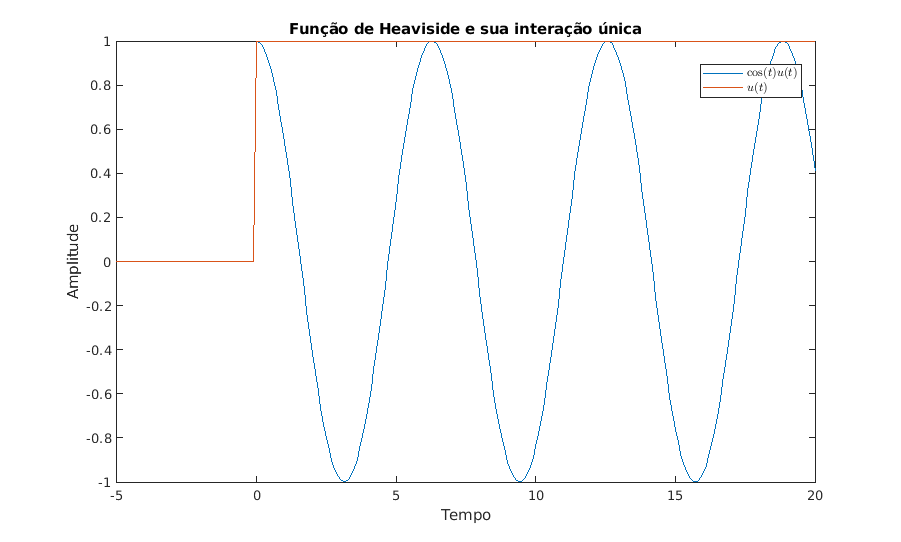
\includegraphics[width=0.95\textwidth]{img/cos(t).png}
    \end{center}

    \item \textbf{Delta de Dirac:} Inicialmente, define-se um pulso unitário $p(t)$ em torno da origem e com área unitária a partir de uma soma de saltos deslocados no tempo, tal que
    \begin{equation}
         p(t) = \dfrac{1}{2a}(u(t+a) - u(t-a)). \label{eq:pulso}
    \end{equation}

    Ao diminuir-se o valor de $a$, percebe-se que o intervalo de tempo em que $p(t)$ ocorre também diminui. No entanto, a restrição da área unitária implica aumento do valor da função para $t \in [-a,a]$. Ao tomar-se o limite em que $a$ tende a zero de $p(t)$, o intervalo de tempo torna-se infinitesimal e a função tende ao infinito.
    Define-se, então, o \textbf{Delta de Dirac} como
    \begin{equation}
        \operatornamewithlimits{lim}_{a \to 0} \dfrac{1}{2a}(u(t+a) - u(t-a)) = \delta(t) =
        \begin{cases}
            \infty, &\quad t=0 \\
            0, &\quad t\neq 0 \\
        \end{cases}, \label{eq:dirac_def}
    \end{equation}
    \noindent mantendo a restrição de área unitária, isto é,
    \begin{equation}
            \displaystyle{\int_{-\infty}^{\infty}{\delta(t)dt}} = 1 \label{eq:dirac_int}
    \end{equation}

    Deste modo, pode-se utilizar o Delta de Dirac para caracterizar eventos pontuais no tempo, a exemplo de forças e descargas elétricas instantâneas. Por isso, também pode ser chamado de função impulso (denotada por $u_0(t)$). A definição do Delta do Dirac resulta em uma propriedade muito útil chamada \textbf{filtragem}, dada por

    $$
        \displaystyle{\int_{-\infty}^{\infty}{f(t)\delta(t)dt}} = f(0),
    $$

    \noindent sendo $f(t)$ uma função contínua em torno da origem. Uma interpretação qualitativa da filtragem é que, devido ao intervalo infinitesimal $t \in [-a,a]$ em que o delta é não nulo, pode-se considerar que o valor de $f(t)$ é aproximadamente $f(0)$, resultando em

    $$
        \displaystyle{\int_{-\infty}^{\infty}{f(t)\delta(t)dt}} \approx
        f(0) \displaystyle{\int_{-\infty}^{\infty}{\delta(t)dt}},
    $$

    \noindent expressão na qual é possível aplicar a definição \eqref{eq:dirac_int}, resultando no próprio valor da função no ponto. Assim como a função salto, é possível aplicar deslocamento no tempo, de modo que exista uma ação impulsiva em um ponto arbitrário $t=t_0$, ou seja,

    $$\delta(t-t_0) =
        \begin{cases}
            \infty, &\quad t=t_0 \\
            0, &\quad t\neq t_0 \\
        \end{cases}.
        $$

    É importante salientar que o Delta de Dirac não é considerado uma função do ponto de vista matemático (apesar de ser comumente referido como tal), pois é definido a partir de um limite de funções. De fato, a integral de uma função infinita em um intervalo de tempo nulo resultaria em indefinição. Entretanto, o problema foi formulado de modo a diminuir o intervalo de tempo com a restrição da área do pulso ser unitária, o que, assintoticamente, leva a ``altura'' do pulso a um valor extremamente grande.

    Informalmente, considera-se o Delta de Dirac como a derivada da função salto. Intuitivamente, percebe-se que em $t=0$ a taxa de variação de $u(t)$ é infinita, e para qualquer $t \neq 0$ a função é constante. Mais especificamente, relembrando que a definição de derivada é dada por

    \begin{equation}
        \dfrac{d}{dt}f(t) = \operatornamewithlimits{lim}_{h \to 0} \label{eq:derivada_def} \dfrac{f(t+h)-f(t)}{h},
    \end{equation}

    \noindent verifica-se que a equação \eqref{eq:dirac_def} é exatamente a definição de derivada, com $f(t)=u(t-a)$ e $h = 2a$. Portanto, sabendo que $a$ tende a zero,

    \begin{equation*}
        \delta(t) = \dfrac{d}{dt} u(t).
    \end{equation*}

    \noindent No entanto, o fato da função salto ser descontínua na origem torna mais razoável considerar que

    \begin{equation*}
        \int_{-\infty}^{t} \delta(\tau)d\tau = u(t),
    \end{equation*}

    \noindent embora ambas definições serem utilizadas frequentemente no contexto de circuitos elétricos.

    \item \textbf{Função Rampa:} consiste em uma reta partindo da origem, com inclinação unitária,

    \begin{equation*}
        R(t) =
        \begin{cases}
            0, &\quad t < 0 \\
            t, &\quad t \geqslant 0 \\
        \end{cases}.
    \end{equation*}

    Fica claro que a função rampa é a primitiva da função salto. Por isso, ao invés de $R(t)$, é comum expressar a rampa como $tu(t)$, ou até mesmo $u_{-2}(t)$. Percebe-se que ao integrar a função rampa, ter-se-á uma função parábola no primeiro quadrante dada por $t^2u(t)$. Este raciocínio pode ser extrapolado para $n$ dimensões, apesar de ser incomum utilizar $n>2$ nas aplicações básicas de circuitos elétricos.

    \item Observação: A notação $u_0(t)$, $u_{-1}(t)$, $u_{-2}(t)$ etc refere-se às respectivas Transformadas de Laplace das funções singulares, dadas pela tabela a seguir.

    \begin{center}
        \begin{tabular}{c|c}
            Tempo & Frequência \\ \hline
            $\delta(t)$ & $1$ \\
            $u(t)$ & $s^{-1}$ \\
            $tu(t)$ & $s^{-2}$ \\
            $t^2u(t)$ & $s^{-3}$
        \end{tabular}
    \end{center}

    Deste modo, o subíndice representa a potência da variável $s$ na frequência. Vale ressaltar que este material tem como foco a análise temporal de circuitos. Esta observação foi feita apenas a título de curiosidade.
\end{itemize}

\subsubsection{Unidades de Medida}
\label{subsubsec:unidades}
\begin{itemize}
    \item \textbf{Ohm [$\Omega$]}: resistência elétrica, é a relação entre a tensão e a corrente em um resistor. Também utilizado como medida de reatância\footnote{A reatância de um capacitor é $X_C=-(\omega C)^{-1}$ e a de um indutor é $X_L=\omega L$, sendo $\omega$ a frequência de excitação da fonte.} e impedância elétrica, tem-se que uma impedância $Z$ segue a expressão $Z = R + jX$, sendo $R$ a resistência, $X$ a reatância e $j$ a unidade imaginária. Em outras palavras, a resistência é a parte real da impedância. Em muitos casos, impedância e resistência são informalmente utilizados como sinônimos, apesar de nem sempre representarem a mesma coisa (de fato, são equivalentes apenas quando não há reatâncias). Tal relação torna-se útil ao trabalhar com circuitos no domínio da frequência, fora do escopo deste material.
    \item \textbf{Siemens [$S$]}: condutância elétrica, inverso da resistência (ou admitância, inverso de impedância). Esta unidade é também conhecida como \textbf{Mho [$\mho$]} ou \textbf{[$\Omega^{-1}$]}.
    \item \textbf{Henry [$H$]}: indutância elétrica, relação entre a tensão e a variação da corrente em um indutor.
    \item \textbf{Farad [$F$]}: capacitância elétrica, relação entre a carga elétrica e a tensão em um capacitor.
    \item \textbf{Joule [$J$]}: energia. Para resistores, corresponde à energia dissipada através do efeito Joule, para capacitores à energia armazenada na forma de um campo elétrico e para indutores à energia armazenada na forma de campo magnético.
    \item \textbf{Watt [$W$]}: potência útil, corresponde à energia dissipada por unidade de tempo. Para resistores, é calculada por $P=V_Ri_R$.
    \item \textbf{Volt-Ampère Reativo [$VAr$]}: potência reativa, corresponde à potência armazenada nos elementos reativos (indutor e capacitor).
    \item \textbf{Volt-Ampère [$VA$]}: potência aparente, corresponde à potência complexa em um circuito de corrente alternada, de forma que $S = P + jQ$, sendo $P$ a potência útil, $Q$ a potência reativa e $j$ a unidade imaginária. A distinção entre tipos de potência torna-se relevante para a análise de circuitos no domínio da frequência, fora do escopo deste material.
\end{itemize}

Além disso, existem alguns prefixos de unidades comuns na análise de circuitos elétricos.

\begin{center}
    Relações dos prefixos das unidades \\
    \begin{tabular}{|c|c|c|} \hline
        Prefixo & Símbolo & Multiplicador \\ \hline
        Pico & $p$ & $10^{-12}$ \\
        Nano & $n$ & $10^{-9}$ \\
        Micro & $\mu$ & $10^{-6}$ \\
        Mili & $m$ & $10^{-3}$ \\
        Kilo & $k$ & $10^{3}$ \\
        Mega & $M$ & $10^{6}$ \\
        Giga & $G$ & $10^{9}$ \\ \hline
    \end{tabular}
\end{center}

Uma importante ferramenta para conferir respostas em circuitos elétricos (e na engenharia, de modo geral) é a chamada \textbf{análise dimensional}, que consiste em, como diz o nome, analisar as dimensões de alguma equação, tendo como princípio que, se ambos os lados são iguais, ambos os lados devem possuir a exata mesma unidade. Tomando como exemplo a fórmula da potência útil $P = Vi$ e utilizando as definições de tensão e corrente da Seção \ref{subsec:variaveis}, tem-se que

\begin{equation}
    P = Vi = \dfrac{dE}{dq} \dfrac{dq}{dt} = \left[\dfrac{J}{C}\dfrac{C}{s}\right] = \left[\dfrac{J}{s}\right] = [W],
\end{equation}

\noindent em que [$\cdot$] representa unidades de medida. Verifica-se que, de fato, existe equivalência de unidades na equação. Caso houvesse disparidade, concluir-se-ía que a equação está incorreta.

\subsubsection{Curto Circuito e Circuito Aberto}
Considera-se um \textbf{curto circuito} um elemento com impedância tendendo a 0 (zero), ou seja, que permite livremente a passagem de corrente e com queda de tensão nula sobre o mesmo. \\
\indent Considera-se um \textbf{circuito aberto} um elemento com impedância tendendo ao infinito, não permitindo a passagem de corrente, mas podendo possuir queda de tensão entre seus terminais.

\subsubsection{Teorema da Reciprocidade}
Considerando um circuito elétrico resistivo com apenas uma fonte de corrente ou tensão, e um instrumento de medição, voltímetro ou amperímetro, é possível permutar a fonte e o instrumento sem modificar a leitura do mesmo. Por exemplo

\noindent\begin{minipage}{\textwidth}
\begin{minipage}[b][5cm][b]{\dimexpr0.5\textwidth-0.5\Colsep\relax}
    \begin{center}
        \begin{tikzpicture}[scale=0.95,transform shape]\draw
            (0,3) to[R,l=$R_1$] (0,0)
            (0,3) to[R,l=$R_2$] (3,3)
            (.5,3) -- (.5,4.5)
            (.5,4.5) to[voltmeter] (2.5,4.5)
            (2.5,4.5) -- (2.5,3)
            (3,3) to[V,l=$e_i$] (3,0)
            (3,3) to[R,l=$R_3$] (6,3)
            (6,3) to[R,l=$R_4$] (6,0)
            (0,0) -- (6,0)
        ;\end{tikzpicture}
    \end{center}
\end{minipage}
\begin{minipage}[b][5cm][b]{\dimexpr0.5\textwidth-0.5\Colsep\relax}
    \begin{center}
        \begin{tikzpicture}[scale=0.95,transform shape]\draw
            (0,3) to[R,l=$R_1$] (0,0)
            (0,3) to[R,l=$R_2$] (3,3)
            (.5,3) -- (.5,4.5)
            (.5,4.5) to[V,l=$e_i$] (2.5,4.5)
            (2.5,4.5) -- (2.5,3)
            (3,3) to[voltmeter] (3,0)
            (3,3) to[R,l=$R_3$] (6,3)
            (6,3) to[R,l=$R_4$] (6,0)
            (0,0) -- (6,0)
        ;\end{tikzpicture}
    \end{center}
\end{minipage}
\end{minipage}

\vspace{0.5cm}
A tensão medida no voltímetro permanece a mesma nos dois casos. O Teorema de Reciprocidade extende-se também para fontes de corrente.

\newpage

\section{Circuitos Não Reativos}
\label{sec:resistivos}

\subsection{Operações básicas}

\subsubsection{Divisor de Tensão}
\label{subsubsec:divten}
Em um circuito série contendo apenas uma fonte de tensão e resistores, pode-se expressar a tensão $V_{R_x}$ em um resistor $R_{x}$ por

\begin{center}
    \begin{tikzpicture}\draw
        (0,3) to[V,l=$V_i$] (0,0)
        (0,3) to[R,l=$R_a$] (3,3)
        (3,3) to[R,l=$R_x$,v=$V_{R_x}$](3,0)
        (0,0) -- (3,0)
    ;\end{tikzpicture}
\end{center}

\begin{equation}
    V_{R_x}=\frac{R_{x}}{R_{eq}}V_{i}=\frac{R_{x}}{R_{x}+R_{a}}V_{i} \hspace{0.45cm}[V]
\end{equation}

\vspace{2mm}

 \textbf{Observação:} Note que tal operação é válida para $N$ resistores em série, uma vez que $R_a$ pode, na verdade, ser a associação em série dos $N-1$ resistores diferentes de $R_x$.

\vspace{4mm}

\justifying

\noindent Para indutores, a equação é análoga, portanto
\begin{equation}
    V_{L_x}=\frac{L_{x}}{L_{eq}}V_{i}=\frac{L_{x}}{L_{x}+L_{a}}V_{i} \hspace{0.45cm}[V]
\end{equation}
Para capacitores, entretanto, a relação entre capacitância e tensão é de proporção inversa, portanto
\begin{equation}
    V_{C_x}=\frac{C_{eq}}{C_{x}}V_{i}=\frac{C_{a}}{C_{x}+C_{a}}V_{i} \hspace{0.45cm}[V]
\end{equation}

\subsubsection{Divisor de Corrente}
\label{subsubsec:divcor}
Em um circuito paralelo contendo apenas uma fonte de corrente e resistores, pode-se expressar a corrente $i_{R_x}$ em um resistor $R_{x}$ por

\begin{center}
    \begin{tikzpicture}\draw
        (0,0) to[I,l=$i_i$] (0,3)
        (0,3) -- (6,3)
        (3,3) to[R,l=$R_x$,f=$i_{R_x}$](3,0)
        (6,3) to[R,l=$R_a$](6,0)
        (0,0) -- (6,0)
    ;\end{tikzpicture}
\end{center}

\begin{equation}
    i_{R_x}=\frac{R_{eq}}{R_{x}}i_{i}=\frac{R_{a}}{R_{x}+R_{a}}i_{i} \hspace{0.45cm}[A]
\end{equation}

\vspace{2mm}

    \textbf{Observação:} Note que tal operação é válida para $N$ resistores em paralelo, uma vez que $R_a$ pode, na verdade, ser a associação em paralelo dos $N-1$ resistores diferentes de $R_x$.

\vspace{4mm}

\justifying

\noindent Para indutores, a relação é análoga
\begin{equation}
    i_{L_x}=\frac{L_{eq}}{L_{x}}i_{i}=\frac{L_{a}}{L_{x}+L_{a}}i_{i} \hspace{0.45cm}[A]
\end{equation}
Para capacitores, a corrente é diretamente proporcional à capacitância, portanto
\begin{equation}
    i_{C_x}=\frac{C_{x}}{C_{eq}}i_{i}=\frac{C_{x}}{C_{x}+C_{a}}i_{i} \hspace{0.45cm}[A]
\end{equation}

\subsubsection{Equivalente de Thévenin e Equivalente de Norton}
\label{subsubsec:thevenin}
O Teorema de Thévenin (também chamado de Equivalente de Thévenin) é uma técnica de simplificação de circuitos que transforma uma rede linear de resistores e fontes (controladas ou não) em um circuito equivalente contendo uma fonte de tensão $E_{th}$ em série com um resistor $R_{th}$. Para tal, deve-se escolher \textbf{dois} terminais de interesse $a$ e $b$.

Considerando uma rede linear genérica que contém apenas fontes e resistores

\noindent\begin{minipage}{\textwidth}
\begin{minipage}[c][4cm][c]{\dimexpr0.45\textwidth-0.5\Colsep\relax}
    \begin{center}
    \begin{tikzpicture}[scale=1.5,transform shape]
        \ctikzset{nodes width=0.025}
        \draw
        node[fourport,t=\tiny{Sub-circuito}](btt){}
        (btt.2) to[short,-*] ++(1,0) node[label={right:$\scriptstyle{b}$}]{}
        (btt.3) to[short,-*] ++(1,0) node[label={right:$\scriptstyle{a}$}]{}
    ;\end{tikzpicture}
\end{center}
\end{minipage}
\begin{minipage}[c][4cm][c]{\dimexpr0.1\textwidth-0.5\Colsep\relax}
    $\iff$
\end{minipage}
\begin{minipage}[c][4cm][c]{\dimexpr0.45\textwidth-0.5\Colsep\relax}
    \begin{center}
    \begin{tikzpicture}[scale=1.5,transform shape, smallR/.style={R, resistors/scale=0.5}, smallV/.style={V, sources/scale=0.65}]
        \ctikzset{nodes width=0.025}
        \draw
        node[fourport](btt){}
        (btt.2) to[short,-*] ++(1,0) node[label={right:$\scriptstyle{b}$}]{}
        (btt.3) to[short,-*] ++(1,0) node[label={right:$\scriptstyle{a}$}]{};
        \draw[dashed] (btt.3) to[smallR,l_=\tiny{$R_{th}$}] ++(-1.05,0)
        to[smallV,l_=\tiny{$E_{th}$}] ++(0,-0.9)
        to[short] (btt.2)
    ;\end{tikzpicture}
\end{center}
\end{minipage}
\end{minipage}

Por definição,
\begin{itemize}
    \item $E_{th}$ é a tensão entre $a$ e $b$ a circuito aberto,
    \item $R_{th}$ é a resistência equivalente medida a partir dos terminais $a$ e $b$ após matar\footnote{Matar uma fonte é um termo informal para ``igualar o valor da fonte a zero''.} as fontes independentes (no caso de existirem fontes dependentes, deve-se utilizar o método descrito em seguida).
\end{itemize}

Deste modo, conseguimos simplificar a configuração do circuito elétrico, facilitando o cálculo de tensão e corrente em qualquer carga aplicada entre os terminais $a$ e $b$. Por exemplo, para encontrar o valor da tensão no capacitor $C$ pode-se aplicar o Teorema de Thévenin nos terminais indicados na figura

\noindent\begin{minipage}{\textwidth}
\begin{minipage}[c][4cm][c]{\dimexpr0.5\textwidth-0.5\Colsep\relax}
    \begin{center}
        \begin{tikzpicture}[scale=0.9,transform shape]\draw
            (0,3) to[V,l=$e_i$] (0,0)
            (0,3) to[R,l=$R_1$] (3,3)
            (3,3) to[R,l=$R_2$] (3,0)
            (3,3) to[R,l=$R_3$] (6,3)
            (6,3) node[label={right:$a$}]{} to[C,l=$C$,v=$e_0$,*-*] (6,0) node[label={right:$b$}]{}
            (0,0) -- (6,0)
        ;\end{tikzpicture}
    \end{center}
\end{minipage}
\begin{minipage}[c][4cm][c]{\dimexpr0.5\textwidth-0.5\Colsep\relax}
    Inicialmente, deve-se abrir o circuito nos terminais do capacitor ($a$ e $b$) e calcular a tensão que cai nos mesmos.
\end{minipage}
\end{minipage}

\noindent\begin{minipage}{\textwidth}
\begin{minipage}[c][4cm][c]{\dimexpr0.5\textwidth-0.5\Colsep\relax}
    \begin{center}
        \begin{tikzpicture}[scale=0.9,transform shape]\draw
            (0,3) to[V,l=$e_i$] (0,0)
            (0,3) to[R,l=$R_1$] (3,3)
            (3,3) to[R,l=$R_2$,v=$V_{ab}$] (3,0)
            (3,3) to[R,l=$R_3$,v=$0V$,f=$0A$,-*] (6,3) node[label={right:$a$}]{}
            (0,0) to[short,-*] (6,0) node[label={right:$b$}]{}
        ;\end{tikzpicture}
    \end{center}
\end{minipage}
\begin{minipage}[c][4cm][c]{\dimexpr0.5\textwidth-0.5\Colsep\relax}
    Como a tensão no resistor $R_3=0$, lembrando que um potencial é o mesmo ao longo de um fio ideal, a tensão $V_{ab}=E_{th}$ é exatamente a tensão que cai no resistor $R_2$, a qual pode ser calculada pelo divisor de tensão
    $$E_{th}=\frac{R_2}{R_1+R_2}e_i$$
\end{minipage}
\end{minipage}

\noindent\begin{minipage}{\textwidth}
\begin{minipage}[c][4cm][c]{\dimexpr0.5\textwidth-0.5\Colsep\relax}
    \begin{center}
    \begin{tikzpicture}[scale=1.5,transform shape, smallR/.style={R, resistors/scale=0.5}, smallV/.style={V, sources/scale=0.65}]
        \ctikzset{nodes width=0.025,voltage/american font=\tiny}
        \draw
        node[fourport](btt){}
        (btt.2) to[short,-*] ++(1,0) node[label={right:$_b$}]{}
        (btt.3) to[short,f=\tiny{$0A$},-*,current arrow scale=24] ++(1,0) node[label={right:$_a$}]{}
        to[open,v=\tiny{$E_{th}$}] ++(0,-0.9);
        \draw[dashed] (btt.3) to[smallR,l_=\tiny{$R_{th}$},v^=\tiny{$0V$}] ++(-1.05,0)
        to[smallV,l_=\tiny{$E_{th}$}] ++(0,-0.9)
        to[short] (btt.2)
    ;\end{tikzpicture}
\end{center}
\end{minipage}
\begin{minipage}[c][4cm][c]{\dimexpr0.5\textwidth-0.5\Colsep\relax}
    Analogamente, olhando para o nosso circuito equivalente de Thévenin, podemos pensar que, ao medirmos a tensão entre os terminais $a$ e $b$ sem que haja corrente, podemos visualizar que estamos medindo diretamente a tensão $E_{th}$, uma vez que não há corrente passando por $R_{th}$ e, portanto, a tensão nele é nula.
\end{minipage}
\end{minipage}

\noindent\begin{minipage}{\textwidth}
\begin{minipage}[c][4cm][c]{\dimexpr0.5\textwidth-0.5\Colsep\relax}
    \begin{center}
        \begin{tikzpicture}[scale=0.9,transform shape]\draw
            (0,3) to[short,*-*] (0,0)
            (0,3) to[R,l=$R_1$] (3,3)
            (3,3) to[R,l=$R_2$] (3,0)
            (3,3) to[R,l=$R_3$,v=$0V$,f=$0A$,-*] (6,3) node[label={right:$a$}]{}
            (0,0) to[short,-*] (6,0) node[label={right:$b$}]{}
        ;\end{tikzpicture}
    \end{center}
\end{minipage}
\begin{minipage}[c][4cm][c]{\dimexpr0.5\textwidth-0.5\Colsep\relax}
    Em seguida, para o cálculo do resistor de Thévenin, mata-se a fonte de tensão (ou seja, deve-se substituí-la por um curto circuito) e calcula-se a resistência equivalente vista dos terminais $a$ e $b$
\end{minipage}
\end{minipage}


\noindent\begin{minipage}{\textwidth}
\begin{minipage}[c][4cm][c]{\dimexpr0.5\textwidth-0.5\Colsep\relax}
    \begin{center}
        \begin{tikzpicture}[scale=0.9,transform shape]\draw
            (0,3) to[R,l=$R_1$] (0,0)
            (0,3) -- (3,3)
            (3,3) to[R,l=$R_2$] (3,0)
            (3,3) to[R,l=$R_3$,-*] (6,3) node[label={right:$a$}]{}
            (0,0) to[short,-*] (6,0) node[label={right:$b$}]{}
        ;\end{tikzpicture}
    \end{center}
\end{minipage}
\begin{minipage}[c][4cm][c]{\dimexpr0.5\textwidth-0.5\Colsep\relax}
    Rearranjando ligeiramente o $R_1$, percebe-se que o resistor equivalente é $R_3$ em série com o paralelo de $R_1$ e $R_2$, ou seja
    $$R_{th}=(R_1//R_2)+R_3=\frac{R_1R_2}{R_1+R_2}+R_3$$
\end{minipage}
\end{minipage}

\noindent\begin{minipage}{\textwidth}
\begin{minipage}[c][4cm][c]{\dimexpr0.5\textwidth-0.5\Colsep\relax}
    \begin{center}
        \begin{tikzpicture}[scale=0.9,transform shape]\draw
            (0,3) to[V,l_=$\dfrac{R_2}{R_1+R_2}e_i$] (0,0)
            (0,3) to[R,l=$(R_1//R_2)+R_3$] (3,3) node[label={right:$a$}]{}
            (3,3) to[C,l=$C$,v=$e_0$,*-*] (3,0) node[label={right:$b$}]{}
            (0,0) -- (3,0)
        ;\end{tikzpicture}
    \end{center}
\end{minipage}
\begin{minipage}[c][4cm][c]{\dimexpr0.5\textwidth-0.5\Colsep\relax}
    Deste modo, é possível escrever o circuito original como um circuito RC série (cuja solução será abordada em capítulos futuros), que torna simples encontrar a saída $e_0$.
\end{minipage}
\end{minipage}

O interessante é que para qualquer combinação de componentes colocada entre os terminais $a$ e $b$ (neste caso é o capacitor), resultará no exato mesmo equivalente de Thévenin, facilitando o cálculo para várias cargas diferentes.

Outra técnica análoga é calcular o Equivalente de Norton, que transforma a rede de componentes em um circuito com uma fonte de corrente $I_{N}$ em paralelo com um resistor $R_{N}$. Neste caso,
\begin{itemize}
    \item $I_{N}$ é a corrente de curto circuito de $a$ para $b$,
    \item $R_{N}$ é a resistência equivalente medida a partir dos terminais $a$ e $b$ após matar as fontes independentes (no caso de existirem fontes dependentes, deve-se utilizar o método descrito em seguida).
\end{itemize}

Tomando-se o mesmo exemplo,

\noindent\begin{minipage}{\textwidth}
\begin{minipage}[c][4cm][c]{\dimexpr0.5\textwidth-0.5\Colsep\relax}
    \begin{center}
        \begin{tikzpicture}[scale=0.9,transform shape]\draw
            (0,3) to[V,l=$e_i$] (0,0)
            (0,3) to[R,l=$R_1$] (3,3)
            (3,3) to[R,l=$R_2$] (3,0)
            (3,3) to[R,l=$R_3$] (6,3)
            (6,3) node[label={right:$a$}]{} to[C,l=$C$,v=$e_0$,*-*] (6,0) node[label={right:$b$}]{}
            (0,0) -- (6,0)
        ;\end{tikzpicture}
    \end{center}
\end{minipage}
\begin{minipage}[c][4cm][c]{\dimexpr0.5\textwidth-0.5\Colsep\relax}
    Deve-se trocar o capacitor por um curto circuito e calcular a corrente que passa de $a$ para $b$.
\end{minipage}
\end{minipage}

    \noindent\begin{minipage}{\textwidth}
    \begin{minipage}[c][4cm][c]{\dimexpr0.5\textwidth-0.5\Colsep\relax}
        \begin{center}
            \begin{tikzpicture}[scale=0.9,transform shape]\draw
                (0,3) to[V,l=$e_i$] (0,0)
                (0,3) to[R,l=$R_1$] (3,3)
                (3,3) to[R,l=$R_2$] (3,0)
                (3,3) to[R,l=$R_3$] (6,3)
                (6,3) to[short,f=$I_N$] (6,0)
                (0,0) -- (6,0)
            ;\end{tikzpicture}
        \end{center}
    \end{minipage}
    \begin{minipage}[c][4cm][c]{\dimexpr0.5\textwidth-0.5\Colsep\relax}
        Neste caso, para calcular a corrente $I_N$, pode-se associar $R_2$ e $R_3$ e em seguida dividir a tensão.
    \end{minipage}
    \end{minipage}

    \vspace{1.2cm}

    \noindent\begin{minipage}{\textwidth}
    \begin{minipage}[c][4cm][c]{\dimexpr0.5\textwidth-0.5\Colsep\relax}
        \begin{center}
            \begin{tikzpicture}[scale=0.9,transform shape]\draw
                (0,3) to[V,l=$e_i$] (0,0)
                (0,3) to[R,l=$R_1$] (3,3)
                (3,3) to[R,l=$R_2//R_3$,v=V] (3,0)
                (0,0) -- (3,0)
            ;\end{tikzpicture}
        \end{center}
    \end{minipage}
    \begin{minipage}[c][4cm][c]{\dimexpr0.5\textwidth-0.5\Colsep\relax}
        $$V=\dfrac{\dfrac{R_2R_3}{R_2+R_3}}{R_1+\dfrac{R_2R_3}{R_2+R_3}}ei$$
        Como a tensão para componentes em paralelos é a mesma que cai em seu equivalente, temos que
        $$I_N=\frac{V}{R_3}=\dfrac{\dfrac{R_2}{R_2+R_3}}{R_1+\dfrac{R_2R_3}{R_2+R_3}}ei$$
    \end{minipage}
    \end{minipage}

    \noindent\begin{minipage}{\textwidth}
    \begin{minipage}[c][4cm][c]{\dimexpr0.5\textwidth-0.5\Colsep\relax}
        \begin{center}
            \begin{tikzpicture}[scale=0.9,transform shape]\draw
                (0,3) to[R,l=$R_1$] (0,0)
                (0,3) -- (3,3)
                (3,3) to[R,l=$R_2$] (3,0)
                (3,3) to[R,l=$R_3$,-*] (6,3) node[label={right:$a$}]{}
                (0,0) to[short,-*] (6,0) node[label={right:$b$}]{}
            ;\end{tikzpicture}
        \end{center}
    \end{minipage}
    \begin{minipage}[c][4cm][c]{\dimexpr0.5\textwidth-0.5\Colsep\relax}
        Para o resistor $R_N$, percebe-se que o resistor equivalente é igual a $R_{th}$, ou seja
        $$R_{N}=R_{th}=(R_1//R_2)+R_3=\frac{R_1R_2}{R_1+R_2}+R_3$$
    \end{minipage}
    \end{minipage}

    \noindent\begin{minipage}{\textwidth}
    \begin{minipage}[c][4cm][c]{\dimexpr0.7\textwidth-0.5\Colsep\relax}
        \begin{center}
            \begin{tikzpicture}[scale=0.9,transform shape]\draw
                (0,0) to[I,l=$\dfrac{\dfrac{R_2}{R_2+R_3}}{R_1+\dfrac{R_2R_3}{R_2+R_3}}ei$] (0,3)
                (0,3) -- (3.5,3)
                (3.5,3) to[R,l_=$(R_1//R_2)+R_3$] (3.5,0)
                (3.5,3) -- (6,3)
                (6,3) node[label={right:$a$}]{} to[C,l=$C$,v=$e_0$,*-*] (6,0) node[label={right:$b$}]{}
                (0,0) -- (6,0)
            ;\end{tikzpicture}
        \end{center}
    \end{minipage}
    \begin{minipage}[c][4cm][c]{\dimexpr0.3\textwidth-0.5\Colsep\relax}
        O circuito se limita a um RC em paralelo.
    \end{minipage}
    \end{minipage}


É possível transformar um equivalente Thévenin em um equivalente Norton e vice-versa escolhendo os terminais $a$ e $b$ da seguinte maneira

\noindent\begin{minipage}{\textwidth}
\begin{minipage}[c][4cm][c]{\dimexpr0.45\textwidth-0.5\Colsep\relax}
    \begin{center}
        \begin{tikzpicture}[scale=0.9,transform shape]\draw
            (0,0) to[I,l=$I_N$] (0,3)
            (0,3) to[short,-*] (4,3) node[label={right:$a$}]{}
            (3,3) to[R,l_=$R_N$] (3,0)
            (0,0) to[short,-*] (4,0) node[label={right:$b$}]{}
        ;\end{tikzpicture}
    \end{center}
\end{minipage}
\begin{minipage}[c][4cm][c]{\dimexpr0.1\textwidth-0.5\Colsep\relax}
    $\iff$
\end{minipage}
\begin{minipage}[c][4cm][c]{\dimexpr0.45\textwidth-0.5\Colsep\relax}
    \begin{tikzpicture}[scale=0.9,transform shape]\draw
        (0,3) to[V,l_=$E_{th}$] (0,0)
        (0,3) to[R,l=$R_{th}$,-*] (3,3) node[label={right:$a$}]{}
        (0,0) to[short, -*] (3,0) node[label={right:$b$}]{}
    ;\end{tikzpicture}
\end{minipage}
\end{minipage}

Utilizando as relações da Lei de Ohm
$$ R_{th}=R_{N} $$
\begin{equation}
    E_{th}=R_{N}I_{N}
\end{equation}
\begin{equation}
    I_{N}=\frac{E_{th}}{R_{th}}
\end{equation}

\subsubsection{Transformação de Fonte}
\label{subsubsec:transform}
É possível utilizar técnicas de simplificação para remodelar blocos fonte-resistor em um circuito, dependendo da conexão entre ditos fonte e resistor. As possíveis combinações são exploradas a seguir.
\vspace{5mm}

\noindent\textbf{Transformações do tipo circuito equivalente}
\vspace{3mm}

Este tipo de transformação de fonte consiste em encontrar o equivalente de Thévenin/Norton de uma fonte e um resistor associados. Como são casos muito usuais, dá-se atenção a fim de que se torne uma ferramenta de uso rápido na resolução de circuitos, sem que seja necessário, de fato, encontrar o equivalente de Thévenin/Norton passo-a-passo.

\vspace{3mm}

\textbf{\small{\textbullet} Fonte de tensão em série com um resistor:}
\begin{center}
    \begin{tikzpicture}\draw
        (0,2) to[V,l=$V$] (0,0)
        (0,2) to[R,l=$R$,-*] (2,2) node[label={right:$a$}]{}
        (0,0) to[short, -*] (2,0) node[label={right:$b$}]{}
    ;\end{tikzpicture}
\end{center}

\noindent Naturalmente, a corrente de curto circuito é $i_{N}=V/R$ e a resistência de Norton é o próprio resistor $R_{N}=R$. Então, uma fonte de tensão $V$ em série com um resistor $R$ é equivalente a uma fonte de corrente $V/R$ em paralelo com um resistor $R$.

\vspace{3mm}

\textbf{\small{\textbullet} Fonte de corrente em paralelo com um resistor:}
\begin{center}
    \begin{tikzpicture}\draw
        (0,0) to[I,l=$I$] (0,2)
        (2,2) to[R,l=$R$] (2,0)
        (0,2) to[short, -*] (3,2) node[label={right:$a$}]{}
        (0,0) to[short, -*] (3,0) node[label={right:$b$}]{}
    ;\end{tikzpicture}
\end{center}
A tensão a circuito aberto é $E_{th}=RI$ e a resistência equivalente é o próprio resistor $R_{th}=R$. Logo, uma fonte de corrente $I$ em paralelo com um resistor $R$ é equivalente a uma fonte de tensão $RI$ em série com um resistor $R$.

Nota-se que as transformações são reversíveis, posto que, como já mencionado na seção anterior, é possível transformar novamente o circuito já transformado.

\noindent\begin{minipage}{\textwidth}
\begin{minipage}[c][4cm][c]{\dimexpr0.45\textwidth-0.5\Colsep\relax}
    \begin{center}
        \begin{tikzpicture}\draw
            (0,0) to[I,l=$I$] (0,2)
            (2,2) to[R,l=$R$] (2,0)
            (0,2) to[short, -*] (3,2) node[label={right:$a$}]{}
            (0,0) to[short, -*] (3,0) node[label={right:$b$}]{}
        ;\end{tikzpicture}
    \end{center}
\end{minipage} \hfill
\begin{minipage}[c][4cm][c]{\dimexpr0.1\textwidth-0.5\Colsep\relax}
    $$\iff$$
\end{minipage} \hfill
\begin{minipage}[c][4cm][c]{\dimexpr0.45\textwidth-0.5\Colsep\relax}
    \begin{center}
        \begin{tikzpicture}\draw
            (0,2) to[V,l=$RI$] (0,0)
            (0,2) to[R,l=$R$,-*] (2,2) node[label={right:$a$}]{}
            (0,0) to[short, -*] (2,0) node[label={right:$b$}]{}
        ;\end{tikzpicture}
    \end{center}
\end{minipage}
\end{minipage}

\vspace{5mm}

\noindent\textbf{Transformações do tipo alteração do circuito}
\vspace{2mm}

É possível também aplicar técnicas simplificadoras que, ao contrário das previamente mostradas, alteram o circuito inicial, resultando em um circuito diferente ao invés de um circuito equivalente. Entretanto, podem ser muito úteis se utilizadas sabiamente, ao conhecer suas limitações. Explicitando, ambas transformações a seguir consistem na retirada de um componente associado a uma fonte, o que apenas altera a potência fornecida pela mesma.

\vspace{2mm}

\textbf{\small{\textbullet} Fonte de tensão em paralelo com um resistor:}

\noindent No caso de haver uma rede de componentes passivos em paralelo com uma fonte de tensão, é possível simplesmente retirá-la sem alteração dos valores de tensão e corrente do resto do circuito, pois, uma vez que a fonte de tensão necessariamente impõe seu valor entre os seus dois terminais, nesse caso $a$ e $b$, sem que essa rede exerça qualquer influência sobre essa tensão. Vale salientar apenas que, dada a natureza da fonte de tensão, em que a corrente é independente e determinada pelo circuito associado à fonte, a corrente fornecida por essa fonte é alterada pela retirada dos componentes passivos e, consequentemente, sua potência também é. Entretanto, se nenhuma dessas duas variáveis, corrente e potência da fonte de tensão, são de interesse para a resolução, é possível aplicar a aproximação.

\noindent\begin{minipage}{\textwidth}
\begin{minipage}[c][4cm][c]{\dimexpr0.45\textwidth-0.5\Colsep\relax}
    \begin{center}
        \begin{tikzpicture}\draw
            (0,2) to[V,l=$V$] (0,0)
            (2,2) to[R,l=$R$] (2,0)
            (0,2) to[short, -*] (3,2) node[label={right:$a$}]{}
            (0,0) to[short, -*] (3,0) node[label={right:$b$}]{}
        ;\end{tikzpicture}
    \end{center}
\end{minipage} \hfill
\begin{minipage}[c][4cm][c]{\dimexpr0.1\textwidth-0.5\Colsep\relax}
    $$\approx$$
\end{minipage} \hfill
\begin{minipage}[c][4cm][c]{\dimexpr0.45\textwidth-0.5\Colsep\relax}
    \begin{center}
        \begin{tikzpicture}\draw
            (0,2) to[V,l=$V$] (0,0)
            (0,2) to[short,-*] (2,2) node[label={right:$a$}]{}
            (0,0) to[short, -*] (2,0) node[label={right:$b$}]{}
        ;\end{tikzpicture}
    \end{center}
\end{minipage}
\end{minipage}

Note que o segundo diagrama foi referido como uma aproximação do primeiro, visto que um elemento foi removido, ao invés de transformado.

\vspace{3mm}

\textbf{\small{\textbullet} Fonte de corrente em série com um resistor:}

\noindent De forma análoga, no caso de haver componentes passivos em série com uma fonte de corrente, é possível retirá-los sem alteração dos valores de tensão e corrente do restante do circuito conectado aos terminais, nesse caso $a$ e $b$, dado que a existência de componentes em série não exerce nenhuma influência sobre a corrente imposta pela fonte de corrente entre seus terminais. Nesse caso, apenas os valores de tensão e a potência na fonte de corrente são alterados pela retirada dos componentes.

\noindent\begin{minipage}{\textwidth}
\begin{minipage}[c][4cm][c]{\dimexpr0.45\textwidth-0.5\Colsep\relax}
    \begin{center}
        \begin{tikzpicture}\draw
            (0,0)node[label={left:$a$}]{} to[I,l=$I$,*-] (2,0)
            (2,0) to[R,l=$R$,-*] (4,0) node[label={right:$b$}]{}
        ;\end{tikzpicture}
    \end{center}
\end{minipage} \hfill
\begin{minipage}[c][4cm][c]{\dimexpr0.1\textwidth-0.5\Colsep\relax}
    $$\approx$$
\end{minipage} \hfill
\begin{minipage}[c][4cm][c]{\dimexpr0.45\textwidth-0.5\Colsep\relax}
    \begin{center}
        \begin{tikzpicture}\draw
            (0,0)node[label={left:$a$}]{} to[I,l=$I$,*-*] (4,0) node[label={right:$b$}]{}
        ;\end{tikzpicture}
    \end{center}
\end{minipage}
\end{minipage}

\subsubsection{Equivalente Thévenin/Norton com fontes controladas}
\label{subsubsec:thfontecontrolada}
Apesar de a maneira de calcular $E_{th}$ e $I_N$ seja a mesma, com a presença de fontes controladas, não é possível calcular $R_{th}$ e $R_N$ por associação de resistores. Por isso, deve-se utilizar uma outra abordagem (que é sempre válida, porém um pouco mais trabalhosa). O método consiste em aplicar uma fonte com um valor conhecido e utilizar a Lei de Ohm para obter o valor do resistor. A mais clássica escolha é calcular a tensão que cai nos terminais de uma fonte de corrente de $1A$. Já que $V=Ri$, para $i=1A$, $V=R$. Do mesmo exemplo dado na Seção \ref{subsubsec:thevenin}, tem-se

\noindent\begin{minipage}{\textwidth}
\begin{minipage}[c][4cm][c]{\dimexpr0.5\textwidth-0.5\Colsep\relax}
    \begin{center}
        \begin{tikzpicture}[scale=0.9,transform shape]\draw
            (0,3) -- (0,0)
            (0,3) to[R,l=$R_1$] (3,3)
            (3,3) to[R,l=$R_2$] (3,0)
            (3,3) to[R,l=$R_3$,-*] (6,3) node[label={right:$a$}]{}
            (0,0) to[short,-*] (6,0) node[label={right:$b$}]{}
            (6,0) to[I,l_=$1A$,v^=$R_{th}$] (6,3)
        ;\end{tikzpicture}
    \end{center}
\end{minipage}
\begin{minipage}[c][4cm][c]{\dimexpr0.5\textwidth-0.5\Colsep\relax}
    Neste caso a tensão que cai na fonte vale $R_{th}$, podendo ser expressada por
    $$R_{th}=[(R_1//R_2)+R_3]\hspace{0.05cm} 1A,$$
    que é o exato mesmo valor encontrado nos outros casos.
\end{minipage}
\end{minipage}

\noindent\begin{minipage}{\textwidth}
\begin{minipage}[c][4cm][c]{\dimexpr0.5\textwidth-0.5\Colsep\relax}
    \begin{center}
    \begin{tikzpicture}[scale=1.5,transform shape, smallR/.style={R, resistors/scale=0.5}, smallI/.style={I, sources/scale=0.65}]
        \ctikzset{nodes width=0.025}
        \draw
        node[fourport](btt){}
        (btt.2) to[short,-*] ++(1,0) node[label={right:$_b$}]{}
        to[smallI,l_=\tiny{$1A$},v^=\tiny{$R_{th}$}] ++(0,0.9)
        (btt.3) to[short,f<=\tiny{$1A$},-*,current arrow scale=24] ++(1,0) node[label={right:$_a$}]{};
        \draw[dashed] (btt.3) to[smallR,l_=\tiny{$R_{th}$},v^=\tiny{$R_{th}$},-*] ++(-1.05,0)
        to[short,-*] ++(0,-0.9)
        to[short] (btt.2)
    ;\end{tikzpicture}
\end{center}
\end{minipage}
\begin{minipage}[c][4cm][c]{\dimexpr0.5\textwidth-0.5\Colsep\relax}
    Novamente, utilizando nosso circuito equivalente de Thévenin, é possível visualizar claramente como medir a tensão em uma fonte de corrente de valor conhecido $i$ nos fornece o valor de $R_{th}$, e o porquê de escolher $i = 1A$ ser tão útil. Vale notar que, como $E_{th}$ é uma combinação linear das fontes de fato presentes no circuito, matá-las, consequentemente, mata $E_{th}$.
\end{minipage}
\end{minipage}

Tomando-se um novo exemplo, com uma fonte controlada de corrente,

\noindent\begin{minipage}{\textwidth}
\begin{minipage}[c][4cm][c]{\dimexpr0.45\textwidth-0.5\Colsep\relax}
    \begin{center}
        \begin{tikzpicture}[scale=0.88,transform shape]\draw
            (0,3) to[V,l=$10V$] (0,0)
            (0,3) to[R,l=$1\Omega$,v=$v$] (3,3)
            (3,0) to[I,l=$3v$] (3,3)
            (3,3) to[R,l=$1\Omega$] (6,3)
            (6,3) node[label={right:$a$}]{} to[C,l=$C$,v=$e_0$,*-*] (6,0) node[label={right:$b$}]{}
            (0,0) -- (6,0)
        ;\end{tikzpicture}
    \end{center}
\end{minipage}
\begin{minipage}[c][4cm][c]{\dimexpr0.1\textwidth-0.5\Colsep\relax}
    $\implies$
\end{minipage}
\begin{minipage}[c][4cm][c]{\dimexpr0.45\textwidth-0.5\Colsep\relax}
    \begin{center}
        \begin{tikzpicture}[scale=0.88,transform shape]\draw
            (0,3) -- (0,0)
            (0,3) to[R,l=$1\Omega$,v=$v$] (3,3)
            (3,0) to[I,l=$3v$] (3,3)
            (3,3) to[R,l=$1\Omega$] (6,3)
            (6,0) node[label={right:$b$}]{} to[I,l_=$1A$,v^=$R_{th}$,*-*] (6,3) node[label={right:$a$}]{}
            (0,0) -- (6,0)
        ;\end{tikzpicture}
    \end{center}
\end{minipage}
\end{minipage}



\noindent\begin{minipage}{\textwidth}
\begin{minipage}[c][5cm][c]{\dimexpr0.5\textwidth-0.5\Colsep\relax}
    \begin{center}
        \begin{tikzpicture}[scale=0.9,transform shape]\draw
            (0,3) -- (0,0)
            (0,3) to[R,l=$1\Omega$,v=$v$,f=$v$] (3,3)
            (3,0) to[I,l=$3v$] (3,3)
            (3,3) to[R,l=$1\Omega$,v<=$1V$,f<=$1A$] (6,3)
            (6,0) node[label={right:$b$}]{} to[I,l_=$1A$,v^=$R_{th}$,*-*] (6,3) node[label={right:$a$}]{}
            (0,0) -- (6,0)
        ;\end{tikzpicture}
    \end{center}
\end{minipage}
\begin{minipage}[c][5cm][c]{\dimexpr0.5\textwidth-0.5\Colsep\relax}
    Através da equação de nó do circuito, tem-se que
    $$v+3v+1=0,$$
    ou seja,
    $$v=-\frac{1}{4}=-0.25V.$$
    Então, pode-se calcular $R_{th}$ utilizando a malha que envolve ambos os resistores e a fonte de $1A$:
    $$R_{th}=1-v=1.25\Omega.$$
\end{minipage}
\end{minipage}

\textbf{Observação:} Formalmente, a definição do resistor de Thévenin é dada pela razão entre a tensão a circuito aberto e a corrente de curto circuito. Entretanto, os autores julgam os métodos aqui apresentados mais eficientes, visto que, em comparação ao cálculo da corrente de Norton, o ato de matar as fontes independentes simplifica significativamente a resolução do circuito.

\vspace{2mm}

Uma outra possibilidade, ainda dentro da ideia de utilizar uma fonte de corrente entre os terminais dos quais deseja-se descobrir a resistência equivalente, útil especificamente no contexto de fontes controladas, é a de aplicar uma fonte de valor inicialmente desconhecido $I$ entre os terminais, e assumir que $I$ é tal que alguma variável de controle existente no circuito assuma um valor específico, tipicamente unitário ou o inverso multiplicativo do ganho da respectiva fonte controlada pela variável, fazendo, dessa forma, com que a fonte controlada também assuma um valor conhecido, podendo servir como atalho na resolução.

Note que pode parecer fácil escolher que $I$ seja tal que a variável de controle assuma valor nulo. Entretanto, ter-se-ia que o próprio valor de $I$ também seria nulo, o que poderia vir a ser uma conclusão frustrante e nada frutífera para resolução do circuito em questão. O leitor pode questionar-se sobre a existência e unicidade do valor $I$ para um dado valor da variável de controle. Pode-se dizer que na análise de circuitos resistivos, a não ser que a variável de controle tenha valor nulo para qualquer valor de $I$ (e.g. a tensão em um curto circuito), para um valor conhecido da variável de controle existe um e apenas um valor de $I$ correspondente. Isso será melhor esclarecido na Seção \ref{subsec:estado}.

Segue um exemplo clássico de aplicação dessa técnica. Apesar de não ser o enfoque deste material, a título de curiosidade, vale dizer que o circuito abaixo representa o modelo de pequenos sinais de um transistor bipolar de junção autopolarizado. Este componente extremamente versátil é utilizado amplamente na indústria de microeletrônica. Enquanto o estudo de transistores faz parte do conteúdo das disciplinas de eletrônica, nossa análise será voltada apenas ao seu circuito equivalente.

\noindent\begin{minipage}{0.95\textwidth}
\begin{minipage}[c][7cm][c]{\dimexpr0.65\textwidth-0.5\Colsep\relax}
    \begin{center}
        \begin{tikzpicture}[scale=0.9,transform shape]\draw
            (0,2) to[C,l=$C$,-*] (0,4) node[label={left:$b$}]{}
            (0,2) to[V=$e_i$,-*] (0,-1)
            node[label={left:$o$}]{}
            (0,4) to[short,f=$i_b$] (2,4)
            (2,4) to[R,l=$R_b$] (2,2)
            (2,2) -- (3,2)
            (3,2) to[R,l=$R_e$] (3,-1)
            (3,2) -- (4,2)
            (4,4) to[I,l_=$\beta i_b$] (4,2)
            (4,4) -- (6,4)
            %(6,4) to[R,l=$R_0$] (6,2)
            (4,2) to[short,-*] (6,2)
            node[label={$e$}]{}
            (8,4) to[R,l=$R_c$,-*] (6,4) node[label={$c$}]{}
            (8,4) to[R,l=$r$] (8,2)
            (8,2) to[V=$V_{cc}$] (8,-1)
            (0,-1) -- (8,-1)
            (0,4) -- (0,6)
            (0,6) to[R,l=$R_{f}$] (8,6)
            (8,6) -- (8,4)
        ;\end{tikzpicture}
    \end{center}
\end{minipage} \hfill
\begin{minipage}[c][7cm][c]{\dimexpr0.35\textwidth-0.5\Colsep\relax}
    Desejando-se saber qual a resistência equivalente vista a partir dos terminais $o$ e $b$, faz-se $V_{cc} = 0$, bem como impõe-se uma fonte de corrente de valor $I$ entre os mesmos terminais, tal que $i_b = 1A$.
\end{minipage}
\end{minipage}

\noindent\begin{minipage}{0.95\textwidth}
\begin{minipage}[c][8cm][c]{\dimexpr0.65\textwidth-0.5\Colsep\relax}
    \begin{center}
        \begin{tikzpicture}[scale=0.9,transform shape]\draw

            (0,-1) to[I,l=$I$,v=$I\cdot R_{th}$,-*] (0,4)
            node[label={left:$b$}]{}
            (0,4) to[short,f=$1A$] (2,4)
            (2,4) to[R,l=$R_b$,v=$ $] (2,2)
            (2,2) -- (3,2)
            (3,2) to[R,l=$R_e$,v=$ $,f=$1+\beta$] (3,-1)
            (3,2) -- (4,2)
            (4,4) to[I,l_=$\beta$] (4,2)
            (4,4) to[short,f<=$\beta$] (6,4)
            (8,4) to[R,l=$R_c$] (6,4)
            (8,4) to[R,l=$r$,v=$ $,-*] (8,2)
            (8,2) to[short,f_=$I-(1+\beta)$,-*] (8,-1)
            (8,-1) to[short,-*] (0,-1) node[label={left:$o$}]{}
            (0,4) -- (0,6)
            (0,6) to[R,l=$R_{f}$,v=$ $,f=$I-1$] (8,6)
            (8,6) -- (8,4)
        ;\end{tikzpicture}
    \end{center}
\end{minipage} \hfill
\begin{minipage}[c][8cm][c]{\dimexpr0.35\textwidth-0.5\Colsep\relax}
    Em seguida, utiliza-se a lei dos nós em $b$ para determinar a corrente que percorre $R_{f}$, bem como, então, no nó entre $R_c$ e $r$ para determinar $i_r$, possibilitando obter $i_{R_e}$ a partir do nó abaixo de $R_e$. Dessa forma, podemos facilmente descobrir o valor de $I$ fazendo a malha que percorre $R_e$, $R_b$, $R_{f}$ e, por fim, $r$, depois isolando $I$ na equação.
\end{minipage}
\end{minipage}

\noindent O valor de $I$ fica, então,

\begin{equation}
    I = \dfrac{R_{f} + R_b + (1+\beta)(R_e + r)}{R_{f}+r}. \label{eq:I_Rth_Fontecontrolada}
\end{equation}

\noindent Por fim, ao fazer a malha percorrendo o potencial do ponto $o$ até o do ponto $b$, passando por $R_b$ e por $R_e$, obtém-se uma equação para $I\cdot R_{th}$. Uma vez que a corrente $I$ é dada por \eqref{eq:I_Rth_Fontecontrolada}, pode-se determinar $R_{th}$, que resulta em

\begin{center}
    $R_{th} = \dfrac{(R_{f}+r)(R_b + (1+\beta)R_e)}{R_{f}+R_b+(1+\beta)(R_e+r)}$.
\end{center}

\noindent Note que o resistor $R_c$ não influencia nos valores de $I$ e $R_{th}$, pois está em série com a fonte controlada de corrente. Convém, portanto, analisar um caso mais completo, em que adiciona-se uma resistência $R_o$ entre os pontos $e$ e $c$ (representando, por exemplo, a não idealidade da fonte controlada), de modo que o resistor $R_c$ não mais seja uma redundância. Assim, o número de variáveis envolvidas no cálculo da resistência de Thévenin aumenta, consequentemente aumentando a complexidade do problema.

\noindent\begin{minipage}{0.95\textwidth}
\begin{minipage}[c][7cm][c]{\dimexpr0.65\textwidth-0.5\Colsep\relax}
    \begin{center}
        \begin{tikzpicture}[scale=0.9,transform shape]\draw
            (0,2) to[C,l=$C$,-*] (0,4) node[label={left:$b$}]{}
            (0,2) to[V=$e_i$,-*] (0,-1)
            node[label={left:$o$}]{}
            (0,4) to[short,f=$i_b$] (2,4)
            (2,4) to[R,l=$R_b$] (2,2)
            (2,2) -- (3,2)
            (3,2) to[R,l=$R_e$] (3,-1)
            (3,2) -- (4,2)
            (4,4) to[I,l_=$\beta i_b$] (4,2)
            (4,4) -- (6,4)
            (4,2) to[short,-*] (6,2)
            node[label={below:$e$}]{}
            (6,2) to[R,l=$R_o$] (6,4)
            (8,4) to[R,l=$R_c$,-*] (6,4) node[label={$c$}]{}
            (8,4) to[R,l=$r$] (8,2)
            (8,2) to[V=$V_{cc}$] (8,-1)
            (0,-1) -- (8,-1)
            (0,4) -- (0,6)
            (0,6) to[R,l=$R_{f}$] (8,6)
            (8,6) -- (8,4)
        ;\end{tikzpicture}
    \end{center}
\end{minipage} \hfill
\begin{minipage}[c][7cm][c]{\dimexpr0.35\textwidth-0.5\Colsep\relax}
    Novamente, desejando-se saber qual a resistência equivalente vista a partir dos terminais $o$ e $b$, faz-se $V_{cc} = 0$, bem como impõe-se uma fonte de corrente de valor $I$ tal que $i_b = 1A$. Também utiliza-se da transformação de fonte para com a fonte de corrente $\beta i_b$ e o resistor $R_o$.
\end{minipage}
\end{minipage}

\noindent\begin{minipage}{0.96\textwidth}
\begin{minipage}[c][8cm][c]{\dimexpr0.63\textwidth-0.5\Colsep\relax}
    \begin{center}
        \begin{tikzpicture}[scale=0.9,transform shape]\draw
            (0,-1) to[I,l=$I$,v=$I\cdot R_{th}$,-*] (0,4)
            node[label={left:$b$}]{}
            (0,4) to[short,f=$1A$] (2,4)
            (2,4) to[R,l=$R_b$,v=$ $] (2,2)
            (2,2) -- (3,2)
            (3,2) to[R,l=$R_e$,v=$ $,f=$1+i_x$] (3,-1)
            (3,2) -- (4,2)
            (4,2) to[V,l_=$\beta R_o$] (4,4)
            (6,4) to[short,f_=\mbox{$i_x=\dfrac{(1-I)R_{f}+R_b+\beta R_o}{R_o+R_c}$}] (4,4)
            (8,4) to[R,l=$R_o + R_c$,v=$ $] (6,4)
            (8,4) to[R,l=$r$,v=$ $,-*] (8,2)
            (8,2) to[short,f_=$I-(1+i_x)$,-*] (8,-1)
            (8,-1) to[short,-*] (0,-1) node[label={left:$o$}]{}
            (0,4) -- (0,6)
            (0,6) to[R,l=$R_{f}$,v=$ $,f=$I-1$] (8,6)
            (8,6) -- (8,4)
        ;\end{tikzpicture}
    \end{center}
\end{minipage} \hfill
\begin{minipage}[c][7cm][c]{\dimexpr0.37\textwidth-0.5\Colsep\relax}
    Feitas essas simplificações, como no circuito anterior, utiliza-se a lei dos nós em $b$ para determinar a corrente que percorre $R_{f}$. Após, tendo que apenas uma das correntes do nó é conhecida, uma possibilidade é utilizar a malha que contém $R_{b}$, $R_{f}$, $R_o + R_c$ e $\beta R_o$ para, justamente, descobrir a tensão em $R_o + R_c$ e, dividindo pelo próprio $R_o + R_c$, descobrir a corrente, $i_x$, nesse resistor. As demais correntes podem ser facilmente obtidas em função de $i_x$, pela lei dos nós.
\end{minipage}
\end{minipage}

\vspace{5mm}
\noindent Alternativamente, a corrente $i_x$ pode ser reescrita em função de $I$ como a equação de uma reta, isto é, $i_x = a_1I + a_0$, sendo $a_1$ e $a_0$ definidos pela equação

\begin{equation}
    i_x=-\dfrac{R_{f}}{R_o+R_c}I + \dfrac{R_{f}+R_b+\beta R_o}{R_o+R_c}, \label{eq:ix_Rth_fonte_arbitraria}
\end{equation}

\noindent o que vem a ser particularmente útil para, além de simplificar a notação, facilitar os cálculos subsequentes, já que busca-se isolar a corrente $I$. Faz-se, então, a malha contendo $R_e$, $\beta R_o$, $R_o + R_c$ e $r$. Note que, apesar de não interferir no resultado final, é uma boa ideia escrever a equação de modo que os termos de $i_x$ sejam todos negativos, já que a dependência em $I$ de $i_x$ é dada pelo coeficiente $a_1 < 0$. Assim, ao substituir a expressão de $i_x$ na equação, todos os termos com $I$ serão positivos. Dessa forma, tem-se a seguinte igualdade:

\begin{equation*}
    -R_e(1+i_x)-(R_o+R_c)i_x+r(I-(1+i_x)) = -\beta R_o.
\end{equation*}

\noindent Separando $i_x$ em função de seus componentes $a_1$ e $a_0$, pode-se isolar $I$, resultando em

\begin{equation*}
    I=\dfrac{-\beta R_o + a_0 (R_e+R_o+R_c+r) + R_e+r}{a_1 (R_e+R_o+R_c+r)+r}.
\end{equation*}

\noindent Aplicando a equação \eqref{eq:ix_Rth_fonte_arbitraria},

\begin{equation}
    I=\dfrac{-\beta R_o + \dfrac{(R_f+R_b+\beta R_o)(R_e+R_o+R_c+r)}{R_o+R_c} + R_e+r}{\dfrac{R_{f}(R_e+R_o+R_c+r)}{R_o+R_c}+r}. \label{eq:I_Rth_fonte_arbitraria}
\end{equation}

\noindent Por fim, uma vez que conhece-se $I$, é possível determinar $R_{th}$ usando a malha contendo a própria fonte $I$, $R_b$ e $R_e$, dada por

\begin{equation*}
    R_{th} = \dfrac{1}{I} [R_b + R_e(1+i_x)].
\end{equation*}

\noindent Escrevendo $i_x$ em função de seus componentes $a_1$ e $a_0$,

\begin{equation*}
    R_{th} = a_1 R_e + \dfrac{1}{I} [R_b + R_e(1+a_0)].
\end{equation*}

\noindent Aplicando, agora, as equações \eqref{eq:ix_Rth_fonte_arbitraria} e \eqref{eq:I_Rth_fonte_arbitraria},

\begin{equation}
    R_{th}= -\dfrac{R_{f}R_e}{R_o+R_c} + \dfrac{\left(\dfrac{R_{f}(R_e+R_o+R_c+r)}{R_o+R_c}+r\right)\left(R_b+R_e + \dfrac{R_e(R_{f}+R_b+\beta R_o)}{R_o + R_c}\right)}{-\beta R_o + \dfrac{(R_f+R_b+\beta R_o)(R_e+R_o+R_c+r)}{R_o+R_c} + R_e+r}.
\end{equation}

\subsubsection{Explosão de Fonte}
\label{subsubsec:explosion}
Explosão de fonte é uma técnica que permite ``deslocar'' uma fonte sem alterar a sua contribuição para com o circuito elétrico. À rigor, apenas reescreve-se o circuito de modo que facilite a resolução. Esta técnica é muitas vezes utilizada juntamente com as transformações para a simplificação de malhas.

\textbf{Fonte de tensão:} Uma fonte de tensão pode ser ``explodida'' em um nó, desde que os mesmos potenciais estejam associados às mesmas cargas.

\begin{center}
\noindent\begin{minipage}{0.8\textwidth}
\begin{minipage}[c][4cm][c]{\dimexpr0.45\textwidth-0.5\Colsep\relax}
    \begin{center}
        \begin{tikzpicture}[scale=0.9,transform shape]\draw
            (0,2) to[V,l=$V$] (0,0)
            (0,2) to[short,-*] (2,2) node[label={above:$b$}]{}
            (0,2) -- (0,4)
            (0,4) to[short,-*] (2,4) node[label={above:$a$}]{}
            (0,0) to[short,-*] (2,0) node[label={above:$c$}]{}
            (2,0) -- (4,0)
            (2,2) to[R,l=$R_b$] (4,2)
            (2,4) to[R,l=$R_a$] (4,4)
            (4,0) -- (4,4)
        ;\end{tikzpicture}
    \end{center}
\end{minipage} \hfill
\begin{minipage}[c][4cm][c]{\dimexpr0.1\textwidth-0.5\Colsep\relax}
    $$\iff$$
\end{minipage} \hfill
\begin{minipage}[c][4cm][c]{\dimexpr0.45\textwidth-0.5\Colsep\relax}
    \begin{center}
        \begin{tikzpicture}[scale=0.9,transform shape]\draw
            (0,2) -- (0,0)
            (2,2) node[label={above:$b$}]{} to[V,l=$V$,*-] (0,2)
            (0,2) -- (0,4)
            (2,4) node[label={above:$a$}]{} to[V,l=$V$,*-] (0,4)
            (0,0) to[short,-*] (2,0) node[label={above:$c$}]{}
            (2,0) -- (4,0)
            (2,2) to[R,l=$R_b$] (4,2)
            (2,4) to[R,l=$R_a$] (4,4)
            (4,0) -- (4,4)
        ;\end{tikzpicture}
    \end{center}
\end{minipage}
\end{minipage}
\end{center}

\vspace{1mm}

Nota-se em ambos os circuitos que os pontos $a$ e $b$ estão sob o potencial positivo de $V$ e que $c$ está na referência. Todas as tensões e correntes são exatamente as mesmas, portanto os circuitos são equivalentes.

Fosse relevante, seria possível transformar as fontes de tensão, agora em série com os resistores, em fontes de correntes em paralelo com suas respectivas cargas. É claro que, neste caso, dada a simplicidade do circuito original, tal simplificação parece redundante e desnecessária, mas, em eventuais e mais complexos problemas, a explosão de fonte pode ser de extrema utilidade.

\vspace{2mm}

\textbf{Fonte de corrente:} Uma fonte de corrente pode ser ``explodida'' em uma malha, desde que as mesmas correntes entrem e saiam de todos os nós.

\begin{center}
\noindent\begin{minipage}{0.8\textwidth}
\begin{minipage}[c][5cm][c]{\dimexpr0.45\textwidth-0.5\Colsep\relax}
    \begin{center}
        \begin{tikzpicture}[scale=0.9,transform shape]\draw
            (0,0) to[I,l=$I$] (4,0)
            (0,2) to[R,l=$R_a$,-*] (2,2) node[label={above:$a$}]{}
            (2,2) to[R,l=$R_b$] (4,2)
            (4,0) -- (4,2)
            (0,0) -- (0,2)
        ;\end{tikzpicture}
    \end{center}
\end{minipage} \hfill
\begin{minipage}[c][5cm][c]{\dimexpr0.1\textwidth-0.5\Colsep\relax}
    $$\iff$$
\end{minipage} \hfill
\begin{minipage}[c][5cm][c]{\dimexpr0.45\textwidth-0.5\Colsep\relax}
    \begin{center}
        \begin{tikzpicture}[scale=0.9,transform shape]\draw
            (0,0) to[I,l=$I$,-*] (2,0)
            node[label={below:$b$}]{}
            (2,0) to[I,l=$I$] (4,0)
            (2,0) to[short,f=$0$] (2,2)
            (0,2) to[R,l=$R_a$,-*] (2,2) node[label={above:$a$}]{}
            (2,2) to[R,l=$R_b$] (4,2)
            (4,0) -- (4,2)
            (0,0) -- (0,2)
        ;\end{tikzpicture}
    \end{center}
\end{minipage}
\end{minipage}
\end{center}

Na segunda figura, percebe-se, pelo nó $b$, que a corrente no fio adicionado é nula. De fato, as cargas $R_a$ e $R_b$ possuem respectivas correntes e tensões idênticas em ambos os casos, o que implica o equivalente ser válido. Pode-se, agora, analogamente à explosão de fonte de tensão, transformar as fontes de corrente em paralelo com os resistores em fontes de tensão em série com suas respectivas cargas.

Para um caso com mais resistores, o processo é exatamente o mesmo. Percebe-se que é possível estender este raciocínio para $n$ resistores e que as correntes nos fios adicionados serão todas nulas. A figura abaixo ilustra uma explosão de fonte de corrente para $n=3$ resistores.

\noindent\begin{minipage}{0.95\textwidth}
\begin{minipage}[c][3cm][c]{\dimexpr0.4\textwidth-0.5\Colsep\relax}
    \begin{center}
        \begin{tikzpicture}[scale=0.9,transform shape]\draw
            (0,0) to[I,l=$I$] (4,0)
            (0,2) to[R,l=$R_b$,-*] (4,2) node[label={above:$b$}]{}
            (4,0) to[R,l=$R_c$,-*] (4,2)
            (0,0) to[R,l=$R_a$,-*] (0,2) node[label={above:$a$}]{}
        ;\end{tikzpicture}
    \end{center}
\end{minipage} \hfill
\begin{minipage}[c][3cm][c]{\dimexpr0.1\textwidth-0.5\Colsep\relax}
    $$\iff$$
\end{minipage} \hfill
\begin{minipage}[c][3cm][c]{\dimexpr0.5\textwidth-0.5\Colsep\relax}
    \begin{center}
        \begin{tikzpicture}[scale=0.9,transform shape]\draw
            (0,0) to[I,l=$I$] (2,0)
            (2,0) to[short,-*] (2,2) node[label={above:$a$}]{}
            (2,0) to[I,l=$I$] (4,0)
            (4,0) to[short,-*] (4,2) node[label={above:$b$}]{}
            (4,0) to[I,l=$I$] (6,0)
            (0,2) to[R,l=$R_b$] (6,2)
            (6,0) to[R,l=$R_c$] (6,2)
            (0,0) to[R,l=$R_a$] (0,2)
        ;\end{tikzpicture}
    \end{center}
\end{minipage}
\end{minipage}

\vspace{2mm}

\textbf{Exemplo:} Para demonstrar a utilidade da explosão de fontes, considera-se o circuito abaixo, dados $R_1=20 \Omega$, $R_2=125 \Omega$, $R_0=400 \Omega$, $C=1 mF$, $\mu = 0.01 \frac{A}{V}$, $e_i=5 u(t)$. Quer-se obter a tensão de saída $e_0(t)$.

\noindent\begin{minipage}{0.95\textwidth}
\begin{minipage}[c][7cm][c]{\dimexpr0.6\textwidth-0.5\Colsep\relax}
    \begin{center}
        \begin{tikzpicture}[scale=0.9,transform shape]\draw
            (0,4) to[V=$e_i$] (0,0)
            (0,4) to[short,-*] (2,4)
            (2,4) to[open,v=$v$] (2,2)
            (2,2) to[short,*-] (3,2)
            (3,2) to[R,l=$R_1$] (3,0)
            (3,2) -- (4,2)
            (4,4) to[I,l_=$\mu v$] (4,2)
            (4,4) -- (6,4)
            (6,4) to[R,l=$R_0$] (6,2)
            (4,2) -- (6,2)
            (6,4) -- (8,4)
            (8,4) to[R,l=$R_2$,v=$e_0$] (8,0)
            (0,0) -- (8,0)
            (0,4) -- (0,6)
            (0,6) to[C,l=$C$] (8,6)
            (8,6) -- (8,4)
        ;\end{tikzpicture}
    \end{center}
\end{minipage} \hfill
\begin{minipage}[c][7cm][c]{\dimexpr0.4\textwidth-0.5\Colsep\relax}
    Devido ao capacitor de realimentação, não é possível encontrar um equivalente de Thévenin em relação aos terminais de $e_0$ (já que só é possível simplificar uma rede linear que contenha apenas resistores e fontes). Porém, pode-se utilizar a explosão de fonte em $e_i$, de modo que:
\end{minipage}
\end{minipage}

\noindent\begin{minipage}{0.95\textwidth}
\hspace{0.01cm}
\begin{minipage}[c][7cm][c]{\dimexpr0.6\textwidth-0.5\Colsep\relax}
    \begin{center}
        \begin{tikzpicture}[scale=0.9,transform shape]\draw
            (0,4) -- (0,0)
            (2,4) to[V,l=$e_i$,*-] (0,4)
            (2,4) to[open,v=$v$] (2,2)
            (2,2) to[short,*-] (3,2)
            (3,2) to[R,l=$R_1$] (3,0)
            (3,2) -- (4,2)
            (4,4) to[I,l_=$\mu v$] (4,2)
            (4,4) -- (6,4)
            (6,4) to[R,l=$R_0$] (6,2)
            (4,2) -- (6,2)
            (6,4) -- (8,4)
            (8,4) to[R,l=$R_2$,v=$e_0$] (8,0)
            (0,0) -- (8,0)
            (0,4) -- (0,6)
            (2,6) to[V,l=$e_i$] (0,6)
            (2,6) to[C,l=$C$] (8,6)
            (8,6) -- (8,4)
        ;\end{tikzpicture}
    \end{center}
\end{minipage} \hfill
\begin{minipage}[c][7cm][c]{\dimexpr0.4\textwidth-0.5\Colsep\relax}
    Analisando os potenciais do circuito, percebe-se que o ramo que contém o capacitor e a fonte está em paralelo com o ramo do resistor $R_2$ (potenciais $e_i$ em um terminal e $0$ em outro), o que permite rearranjar o circuito sem afetar os valores de tensão e corrente no mesmo.
\end{minipage}
\end{minipage}

\begin{center}
    \begin{tikzpicture}[scale=0.9,transform shape]\draw
        (0,4) -- (0,0)
        (2,4) to[V,l=$e_i$,*-] (0,4)
        (2,4) to[open,v=$v$] (2,2)
        (2,2) to[short,*-] (3,2)
        (3,2) to[R,l=$R_1$] (3,0)
        (3,2) -- (4,2)
        (4,4) to[I,l_=$\mu v$] (4,2)
        (4,4) -- (6,4)
        (6,4) to[R,l=$R_0$] (6,2)
        (4,2) -- (6,2)
        (6,4) to[short,-*] (7,4) node[label={above:$a$}]{}
        (7,4) -- (8,4)
        (8,4) to[R,l=$R_2$,v=$e_0$] (8,0)
        (0,0) to[short,-*] (7,0) node[label={above:$b$}]{}
        (7,0) -- (10,0)
        (10,4) -- (8,4)
        (10,2) to[V,l=$e_i$] (10,0)
        (10,4) to[C,l=$C$] (10,2)
    ;\end{tikzpicture}
\end{center}

\noindent Com o circuito escrito nesse formato, pode-se calcular um equivalente de Thévenin, já que tanto a saída $e_0$ quanto o capacitor estão à direita de $a$ e $b$, terminais escolhidos para o Thévenin.

\begin{center}
    \begin{tikzpicture}\draw
        (0,4) to[V,l=$e_i$] (0,0)
        (2,4) to[short,*-] (0,4)
        (2,4) to[open,v=$v$] (2,2)
        (2,2) to[short,*-] (3,2)
        (3,2) to[R,l=$R_1$,v=$0V$] (3,0)
        (3,2) to[short,f<=$0A$] (4,2)
        (4,4) to[I,l_=$\mu v$,-*] (4,2) node[label={below:$s$}]{}
        (4,4) -- (6,4)
        (6,4) to[R,l=$R_0$,v<=$\mu R_0v$] (6,2)
        (4,2) to[short,f_=$\mu v$] (6,2)
        (6,4) to[short,f=$0A$,-*] (8,4) node[label={right:$a$}]{}
        (0,0) to[short,f_<=$0A$,-*] (3,0) node[label={below:$o$}]{}
        (3,0) to[short,f_=$0A$] (7,0)
        (7,0) to[short,-*] (8,0) node[label={right:$b$}]{}
        (7.9,4) to[open,v=$E_{th}$] (7.9,0)
    ;\end{tikzpicture}
\end{center}

\noindent Já que a corrente em um circuito aberto é igual a $0A$, utilizando o nó $o$, descobre-se que a corrente no resistor $R_1$ é, também, igual a $0A$, o que implica tensão $0V$ no mesmo. Então, através da análise do nó $s$, percebe-se que a corrente da fonte controlada é igual à do resistor $R_0$, polarizando-o como mostrado no circuito.
A partir daí, pode-se calcular $E_{th}$ pela malha que contém $R_0$ e $R_1$, ou seja

$$E_{th}=-\mu R_0v.$$
%TODO: Falar sobre a dependência de v
Porém, devemos relacionar a tensão $v$ do elemento controlado com a entrada $e_i$, para manter nosso equivalente diretamente relacionado com a fonte independente, pois a variável de controle não estará presente no circuito resultante. Isso é alcançável utilizando a malha que contém $e_i$, $v$ e $R_1$:

$$e_i=v+0,$$

\noindent ou seja,

$$E_{th}=-\mu R_0e_i$$
$$E_{th}=-20V.$$

\noindent A seguir, para calcular o resistor $R_{th}$, aplica-se uma fonte de $1A$ entre os terminais $a$ e $b$ e mata-se as fontes independentes (neste caso, $e_i$).

\begin{center}
    \begin{tikzpicture}\draw
        (0,1.5) -- (0,0)
        (0,1.5) to[short,*-*] (0,3)
        (0,3) -- (0,4)
        (2,4) to[short,*-] (0,4)
        (2,4) to[open,v=$v$] (2,2)
        (2,2) to[short,*-] (3,2)
        (3,2) to[R,l=$R_1$,v=$R_1$] (3,0)
        (3,2) to[short] (4,2)
        (4,4) to[I,l_=$\mu v$,-*] (4,2) node[label={below:$s$}]{}
        (4,4) -- (6,4)
        (6,4) to[R,l=$R_0$,v<=$ $] (6,2)
        (4,2) to[short,f_=$\mu v - 1$] (6,2)
        (6,4) to[short,-*] (8,4) node[label={right:$a$}]{}
        (0,0) to[short,f_<=$0A$,-*] (3,0) node[label={below:$o$}]{}
        (3,0) to[short] (7,0)
        (7,0) to[short,-*] (8,0) node[label={right:$b$}]{}
        (8,0) to[I,l=$1A$,v=$R_{th}$] (8,4)
    ;\end{tikzpicture}
\end{center}

\noindent Neste caso, a corrente em $R_1$ é $1A$, portanto sua tensão é $R_1$, o que resulta, pela malha à esquerda, na relação

$$v=-R_1.$$

\noindent Além disso, pelo nó $s$, evidencia-se que a corrente no resistor $R_0$, polarizada conforme a imagem, deve ser $i_{R_0}=\mu v - 1$. Portanto, equacionando a malha à direita,

$$R_{th}=R_1-R_0[\mu v-1]=R_1-R_0[-\mu R_1-1]$$
$$R_{th}=R_1+R_0+\mu R_0R_1$$
$$R_{th}=500 \Omega.$$

\noindent Calculado o equivalente, o circuito resultante é

\begin{center}
    \begin{tikzpicture}\draw
        (0,3) to[V,l_=$E_{th}$] (0,0)
        (0,3) to[R,l=$R_{th}$] (2,3)
        (2,3) to[R,l=$R_2$,v=$e_0$] (2,0)
        (2,3) -- (4,3)
        (4,3) to[C,l=$C$] (4,1.5)
        (4,1.5) to[V,l=$e_i$] (4,0)
        (0,0) -- (4,0)
    ;\end{tikzpicture}
\end{center}

\noindent É evidente que a nova forma do circuito é muito mais simples em comparação à original, tornando fácil encontrar $e_0(t)$. Este exemplo será revisitado e concluído na Seção \ref{sec:reativos}, visto que envolve a resolução de um circuito reativo.

%Here

\subsubsection{Balanço de Potência}
\label{subsubsec:balancodepot}
A partir do conceito da conservação de energia, é possível equacionar a potência dos $n$ componentes de um circuito elétrico através da relação
\begin{equation}
    \sum_{k=1}^{n} P_k = 0,
\end{equation}

\noindent o que nos permite fazer um balanço de potências, ou seja, calcular as potências individuais de cada componente e somá-las, visto que a energia total de um sistema será sempre conservada. Naturalmente, a potência é separada em \textbf{fornecida} e \textbf{dissipada}, tornando prático definir uma convenção de sinais para $P_k$, sendo que
\begin{itemize}
    \item \hspace{0.2cm} $P_k > 0$: a potência é \textbf{dissipada} quando as cargas elétricas passam de um ponto de \textbf{maior} potencial elétrico para um de \textbf{menor} potencial elétrico. Em outras palavras, quando a corrente flui do terminal polarizado positivamente $(+)$ para o polarizado negativamente $(-)$, pode-se dizer que o componente ``consumiu'' potência do sistema.
    \item \hspace{0.2cm} $P_k < 0$: A potência é \textbf{fornecida} quando as cargas elétricas passam de um ponto com \textbf{menor} potencial elétrico $(-)$ para um de \textbf{maior} potencial elétrico $(+)$. Neste caso, pode-se dizer que o elemento ``forneceu'' potência elétrica para o sistema.
\end{itemize}

Em geral, utiliza-se do balanço de potência para circuitos resistivos, já que para capacitores e indutores a potência pode (e normalmente vai) variar no tempo. Ainda assim, essa técnica mostra-se útil para rapidamente conferir se a resolução do circuito foi feita de forma correta, já que a energia deve sempre ser conservada em um circuito elétrico.

É importante pontuar que o fato de o componente ser uma fonte (de tensão ou de corrente, controlada ou não) não necessariamente implica que o mesmo forneça potência. Deve-se observar o sentido da corrente em relação à tensão do componente e ater-se à convenção já definida. Por exemplo, considere o seguinte circuito:

\begin{center}
    \begin{tikzpicture}\draw
        (0,3) to [V,l=$e_1$] (0,0)
        (0,3) to [R,l=$R$,f=$i_0$,v=$e_0$] (3,3)
        (3,3) to [V,l=$e_2$] (3,0)
        (0,0) -- (3,0)
        ;
    \end{tikzpicture}
\end{center}

\noindent A tensão no resistor, polarizada conforme a figura, é dada por $e_0 = e_1 - e_2$, sendo a corrente obtida dividindo $e_0$ pela resistência $R$. É claro que o real sentido de $i_0$ depende dos valores das fontes (i.e. se $i_0$ tiver valor negativo, significa que a mesma flui no sentido anti-horário). Atribuindo $R=10\Omega$, $e_1 = 20V$ e $e_2=10V$, tem-se

\begin{center}
    \begin{tikzpicture}\draw
        (0,3) to [V,l=$20V$] (0,0)
        (0,3) to [R,l=$10\Omega$,f=$1A$,v=$10V$] (3,3)
        (3,3) to [V,l=$10V$] (3,0)
        (0,0) -- (3,0)
        ;
    \end{tikzpicture}
\end{center}

\noindent Encontradas as incógnitas do circuito, pode-se computar a potência de cada componente. Note que, seguindo a convenção de sinais, como $i_0$ flui do potencial positivo para o negativo de $e_2$, a fonte consome potência, resultando nas expressões

$$ P_R = 10W, \quad P_{e_1} = -20W, \quad P_{e_2} = 10W.$$

\noindent Ao realizar o balanço, percebe-se que o somatório de potências é igual a zero, o que indica que a energia do sistema foi conservada. Alterando os valores das fontes de modo que $\widehat{e_1}=15V$ e $\widehat{e_2}=20V$, mantendo as polaridades, o novo circuito é

\begin{center}
\noindent\begin{minipage}{0.8\textwidth}
\begin{minipage}[c][5cm][c]{\dimexpr0.45\textwidth-0.5\Colsep\relax}
    \begin{center}
        \begin{tikzpicture}\draw
        (0,3) to [V,l=$15V$] (0,0)
        (0,3) to [R,l=$10\Omega$,f=$-0.5A$,v=$-5V$] (3,3)
        (3,3) to [V,l=$20V$] (3,0)
        (0,0) -- (3,0)
        ;
        \end{tikzpicture}
    \end{center}
\end{minipage} \hfill
\begin{minipage}[c][5cm][c]{\dimexpr0.1\textwidth-0.5\Colsep\relax}
    $$\iff$$
\end{minipage} \hfill
\begin{minipage}[c][5cm][c]{\dimexpr0.45\textwidth-0.5\Colsep\relax}
    \begin{center}
        \begin{tikzpicture}\draw
        (0,3) to [V,l=$15V$] (0,0)
        (0,3) to [R,l=$10\Omega$,f<=$0.5A$,v<=$5V$] (3,3)
        (3,3) to [V,l=$20V$] (3,0)
        (0,0) -- (3,0)
        ;
        \end{tikzpicture}
    \end{center}
\end{minipage}
\end{minipage}
\end{center}

\noindent Neste caso, as potências são

$$ \widehat{P_R} = 2.5W, \quad \widehat{P_{e_1}} = 7.5W, \quad \widehat{P_{e_2}} = -10W,$$

\noindent indicando que, agora, a fonte $\widehat{e_2}$ fornece potência para os demais componentes. Outra observação importante é que em ambos os casos o resistor $R$ dissipou potência, já que a polarização da tensão em resistores é dada pela corrente e vice-versa, ou seja, componentes resistivos sempre dissipam potência (facilmente verificável pelo efeito Joule, que expressa o calor gerado em um resistor percorrido por corrente).

\textbf{Nota:} Apesar da convenção de sinais apresentada ser amplamente utilizada, a mesma não é universal. O importante é que o leitor saiba distinguir as diferenças entre as potências fornecida e dissipada. Particularmente, os autores calculam separadamente as potências fornecida e dissipada e, então, checam se existe igualdade entre ambos os valores. Desta forma, não é necessário utilizar nenhuma convenção de sinais, mas sim aplicar propriamente os conceitos de potência.

\subsection{Teorema da Máxima Transferência de Potência}
\label{subsec:maxpot}

Considerando uma rede elétrica linear contendo apenas resistores e fontes que alimenta uma carga resistiva $R_L$, pela teoria discutida na Seção \ref{subsubsec:thevenin}, é possível encontrar um equivalente para dito circuito em relação à carga, resultando no modelo abaixo.

\begin{center}
    \begin{tikzpicture}
        \draw
            (0,3) to[V_=$E_{th}$] (0,0)
            (0,3) to[R,l=$R_{th}$,f=$i$] (3,3)
            (3,3) to[R,l=$R_L$,v=$V$] (3,0)
            (0,0) -- (3,0)
        ;
    \end{tikzpicture}
\end{center}

\noindent Assim, é possível calcular a potência dissipada na carga através da relação $P = Vi$. Além disso, por divisor de tensão e pela Lei de Ohm, as expressões de tensão e corrente podem ser desenvolvidas de forma que

\begin{equation}
    P = \dfrac{R_L}{R_L+R_{th}}E_{th} \dfrac{1}{R_L+R_{th}}E_{th} = \dfrac{R_L}{(R_L+R_{th})^2}E_{th}^2. \label{eq:maxtransfpot}
\end{equation}

\noindent Como a potência em resistores é sempre dissipada, bem como sua resistência sempre positiva, dado um equivalente de Thévenin, conclui-se que existe um valor máximo de potência na carga para $0 < R_L < \infty$ no ponto que satisfaz a equação diferencial

\begin{equation*}
    \dfrac{\partial}{\partial R_L}P(R_L) = 0.
\end{equation*}

\noindent Derivando a expressão \eqref{eq:maxtransfpot}, tem-se

\begin{equation*}
    \left(\dfrac{1}{(R_L+R_{th})^2} - \dfrac{2R_L}{(R_L+R_{th})^3}\right)E_{th}^2 = 0.
\end{equation*}

\noindent Por ser uma constante, é possível dividir ambos os lados por $E_{th}^2$. Multiplicando, também, ambos os lados por $(R_L+R_{th})^3$, resulta em

\begin{equation*}
    (R_L+R_{th}) - 2R_L = 0,
\end{equation*}

\noindent o que implica

\begin{equation}
    R_L = R_{th}.
\end{equation}

Ou seja, a máxima transferência de potência ocorre quando a carga é exatamente igual ao resistor equivalente de Thévenin.

\subsection{Notação Potencial}
\label{subsec:notpot}

Devido à grande quantidade de componentes envolvidos nas análises de circuitos eletrônicos (que contêm diodos, amplificadores operacionais, transistores etc), é comum desenhar os diagramas utilizando uma notação mais compacta, conhecida como \textbf{notação potencial}. Para tal, omite-se as fontes cuja tensão é medida em relação a uma referência comum (em geral o terra (GND), por ser um ponto de potencial nulo), representando-as através de um potencial. Segue um exemplo ilustrativo.

\begin{center}
\noindent\begin{minipage}{\textwidth}
\begin{minipage}[c][5cm][c]{\dimexpr0.45\textwidth-0.5\Colsep\relax}
    \begin{center}
        \begin{tikzpicture}[scale=0.85,transform shape]\draw
            (0,3) to[V,l=$e_i$] (0,0)
            (0,3) to[R,l=$R_1$] (3,3)
            (3,3) to[R,l=$R_2$] (3,0)
            (3,3) to[R,l=$R_3$] (6,3)
            (6,3) to[C,l=$C$] (6,0)
            (0,0) -- (6,0)
        ;\end{tikzpicture}
    \end{center}
\end{minipage} \hfill
\begin{minipage}[c][5cm][c]{\dimexpr0.1\textwidth-0.5\Colsep\relax}
    $$\iff$$
\end{minipage} \hfill
\begin{minipage}[c][5cm][c]{\dimexpr0.45\textwidth-0.5\Colsep\relax}
    \begin{center}
    \begin{tikzpicture}[scale=0.85, transform shape]\draw
            (0,3) node[label={left:$e_i$}]{} to[R,l=$R_1$,*-] (3,3)
            (3,3) to[R,l=$R_2$] (3,0) node[tlground]{}
            (3,3) to[R,l=$R_3$] (5,3)
            (5,3) to[C,l=$C$] (7,3) node[tlground,rotate=90]{}
            ;
    \end{tikzpicture}
\end{center}
\end{minipage}
\end{minipage}
\end{center}

Perceba que a fonte $e_i$ foi retirada e substituída pela definição de um potencial de mesma intensidade à esquerda de $R_1$. A conexão com a referência dos componentes $R_2$ e $C$ foram representadas por dois terras, tornando desnecessário o desenho do longo fio inferior do primeiro esquema. Vale citar que a representação do capacitor na horizontal no segundo circuito não influencia em nada na resolução do mesmo.

Analogamente à notação usual, a menos que explicitado o contrário, considera-se que todos os potenciais (e tensões) são medidos a partir do terra. No entanto, na notação potencial é frequente a necessidade de explicitar algum terra em função de nenhum terminal ficar incorretamente desconectado (a exemplo do resistor $R_2$ e do capacitor $C$).

\subsection{Diodos}
\label{subsec:diodos}
Um diodo é um elemento não linear composto por semicondutores (geralmente cristais de silício ou germânio) polarizados através de lacunas em duas regiões, uma do tipo N e outra do tipo P, que, na maioria das vezes, permite fácil passagem de corrente em polarização direta e impede a passagem de corrente em polarização reversa. Existem diversos modelos de diodos: desde o diodo ideal, o diodo real (maior nível de complexidade, porém útil em casos que requerem alta precisão) e os diodos Zener e de Schottky. Neste material, consta uma breve explicação sobre o funcionamento do diodo ideal, bem como uma noção estendida para diodos genéricos.

\subsubsection{Diodos Ideais}
\label{subsubsec:diodos}
Os diodos ideais funcionam exclusivamente como elemento de chaveamento. Assume-se que, em condução, o diodo possui queda de tensão $V_{D}=0V$, ou seja, é um curto circuito. Em polarização reversa, entretanto, o diodo ideal se comporta como uma impedância infinita (circuito aberto), impossibilitando a passagem de corrente entre seus terminais. O modelo do diodo ideal é ilustrado pela figura abaixo.
\begin{center}
    \begin{tikzpicture}\draw
        (0,0) to[D,v=$V$,f=$i$,*-*] (3,0)
    ;\end{tikzpicture}
\end{center}

Se o efeito de $V$ polarizar o diodo diretamente ($V>0$), diz-se que o diodo está no modo \textbf{ON} (conduz) e tem-se $i>0$. Neste caso, ao constatar que o diodo está conduzindo, pode-se substituí-lo por um curto circuito, visto que ele permitirá a passagem da corrente sem alterar a tensão do circuito. Do contrário, estando o diodo em polarização reversa ($V<0$), o mesmo opera no modo \textbf{OFF} (não conduz) e seu comportamento é o de uma impedância infinita, isto é, um circuito aberto, não permitindo a passagem de corrente, ou seja, $i=0$.

\vspace{2mm}

\textbf{Exemplo 1:} Determine se o diodo está em condução e calcule a tensão $v$. Considere $R=5\Omega$ e os valores das fontes no SI.
%Here TH ou Delta-Y (prob sec)
\begin{center}
    \begin{tikzpicture}\draw
        (0,2) to[V,l=$80$] (0,0)
        (0,2) to[D,l=$D$] (2,2)
        (2,2) to[R,l=$3R$] (4,2)
        (4,2) to[R,l=$2R$] (4,0)
        (4,2) to[R,l=$R$] (6,2)
        (6,2) to[R,l=$2R$] (6,0)
        (6,2) to[R,l=$2R$] (8,2)
        (8.15,2) to[open,v=$v$] (8.15,0)
        (8,2) to[R,l=$4R$] (10,2)
        (10,2) to[R,l=$4R$] (10,0)
        (0,2) -- (0,4)
        (10,2) -- (10,4)
        (10,4) to[I,l=$2$] (0,4)
        (0,0) -- (10,0)
        ;
    \end{tikzpicture}
\end{center}

\textbf{Exemplo 2:} Encontre a expressão da saída em função da entrada $e_0(e_1)$ para $-\infty < e_1 < \infty$. Dados: $R=10k\Omega$, $e_2=-15V$.

\begin{center}
\noindent\begin{minipage}{\textwidth}
\begin{minipage}[c][5cm][c]{\dimexpr0.45\textwidth-0.5\Colsep\relax}
    \begin{center}
    \begin{tikzpicture}[scale=0.85, transform shape]\draw
        (0,4) to[V,l=$e_1$] (0,0)
        (0,4) to[R,l=$R$] (2,4)
        (2,4) to[R,l=$R$] (4,4)
        (4,4) to[R,l=$R$] (6,4)
        (2,2) to[D,l_=$D_1$] (2,4)
        (4,4) to[D,l=$D_2$] (4,2)
        (2,2) -- (4,2)
        (3,2) node[label={above:$e_0$}]{} to[R,l=$R$,*-] (3,0)
        (6,4) to[V,l=$e_2$] (6,0)
        (0,0) -- (6,0)
        ;
    \end{tikzpicture}
\end{center}
\end{minipage} \hfill
\begin{minipage}[c][5cm][c]{\dimexpr0.1\textwidth-0.5\Colsep\relax}
    $$\iff$$
\end{minipage} \hfill
\begin{minipage}[c][5cm][c]{\dimexpr0.45\textwidth-0.5\Colsep\relax}
    \begin{center}
    \begin{tikzpicture}[scale=0.85, transform shape]\draw
        (0,4) node[label={left:$e_1$}]{} to[R,l=$R$,*-] (2,4)
        (2,4) to[R,l=$R$] (4,4)
        (4,4) to[R,l=$R$,-*] (6,4) node[label={right:$e_2$}]{}
        (2,2) to[D,l_=$D_1$] (2,4)
        (4,4) to[D,l=$D_2$] (4,2)
        (2,2) -- (4,2)
        (3,2) node[label={above:$e_0$}]{} to[R,l=$R$,*-] (3,0) node[tlground]{}
        ;
    \end{tikzpicture}
\end{center}
\end{minipage}
\end{minipage}
\end{center}

Note que ao passar o circuito para notação potencial (referida na Seção \ref{subsec:notpot}), ambas as fontes de tensão foram trocadas por potenciais de mesmas respectivas intensidades, visto que seus valores eram dados em relação à referência nula. Da mesma forma, o terminal do resistor na vertical $R$ que o conectava a $e_1$ e $e_2$ foi substituído pelo próprio terra.

\subsection{Amplificador Operacional Ideal}
\label{subsec:ampop}
Um amplificador operacional (AmpOp) é um componente que tem como saída um sinal de entrada amplificado. No caso ideal, considera-se o ganho $A=V_o/V_i$ infinito. Este componente possui dois terminais de entrada, as portas inversora $(-)$ e não inversora $(+)$ e um terminal de saída, além de dois terminais de alimentação $(+V_{CC}$ e $-V_{CC})$. Idealmente o AmpOp possui uma impedância de entrada infinita (correntes iguais a zero em sua entrada), bem como uma impedância de saída zero (não há perda alguma de tensão), ou seja, um sinal de tensão é perfeitamente amplificado para a saída, sem nenhum tipo de perda.

\begin{center}
    \begin{tikzpicture} \draw
        (0,0) node[op amp] (opamp) {}
        (opamp.+) to [short,-*] (-1.5,-0.49) node[left] {$V_+$}
        (opamp.-) to [short,-*] (-1.5,0.49) node[left] {$V_-$}
        (opamp.out) to [short,-*] (1.6,0) node[right] {$V_o$}
        (opamp.up) ++ (0,0.5) node[above] {$+V_{CC}$} to [short,*-] (opamp.up)
        (opamp.down) ++ (0,-0.5) node[below] {$-V_{CC}$} to [short,*-] (opamp.down)
        ;
    \end{tikzpicture}
\end{center}

É evidente que no mundo real não é possível obter ganho infinito ou impedâncias infinitas ou zero. O que realmente acontece é que, a partir de um certo ponto, a tensão de saída do amplificador operacional é saturada de acordo com as tensões de alimentação. A impedância de entrada é muito alta e a impedância de saída é muito baixa. Neste material, considerar-se-á apenas a característica \textbf{ideal} dos amplificadores operacionais.

Os amplificadores operacionais possuem diversas aplicações, sendo a mais básica delas um comparador de tensão (o maior valor entre $V_{+}$ e $V_{-}$ será amplificado, saturando a saída em $+V_{CC}$ ou $-V_{CC})$. Em grande parte das aplicações, utiliza-se de uma configuração em \textbf{malha fechada}, quando o circuito é realimentado (feedback). As aplicações a seguir utilizam a realimentação negativa, ou seja, a saída do AmpOp é conectada à entrada inversora através de uma rede de componentes. Note que os pinos de alimentação serão omitidos daqui em diante.

\begin{center}
    \begin{tikzpicture}\draw
        (0,0) node[op amp] (opamp) {}
        (opamp.+) to [short, -*] (-2.5,-0.5) node[left] {$V_+$}
        (opamp.-) -- (-1.5,0.49)
        (opamp.out) -- (1.2,1.5) -- (-1.5,1.5) -- (-1.5,0.49) to [short,-*] (-2.5,0.5) node[left] {$V_-$}
        (opamp.out) to [short,-*] (1.8,0) node[right] {$V_o$}
        ;
    \end{tikzpicture}
\end{center}

Esta ligação tem como característica a criação do chamado \textbf{curto circuito virtual} entre seus terminais. Em outras palavras, a tensão entre as entradas inversora e não inversora é igual a zero. Lembrando que, como a impedância de entrada é muito alta, considera-se a corrente de entrada igual a zero.

\subsubsection{Configuração Inversora}
A aplicação de tensão na porta inversora causa um ganho proporcional e com sinal oposto em relação à entrada. Para um caso genérico:

\begin{center}
    \begin{tikzpicture}\draw
        (0,0) node[op amp] (opamp) {}
        (opamp.+) -- (-1.5,-0.49) node[ground] {}
        (opamp.-) -- (-2,0.49) to [R,l_=$R_i$,-*] (-5,0.49) node[left] {$V_i$}
        (opamp.out) -- (1.2,2) to [R,l_=$R_f$] (-2,2) -- (-2,0.49)
        (opamp.out) to [short,-*] (1.8,0) node[right] {$V_o$}
        ;
    \end{tikzpicture}
\end{center}

\begin{equation}
    A=\frac{V_{o}}{V_{i}}=-\frac{R_{f}}{R_{i}}  \label{eq:ampop_inversor}
\end{equation}

\textbf{Dedução:} Como o amplificador operacional está em realimentação negativa, a tensão entre sua entradas é nula. Assim, já que a porta não inversora está aterrada, o potencial na porta inversora será igual a zero. Logo, a tensão que cai no resistor $R_i$ é igual a $V_i$. Tendo que a impedância de entrada do amplificador operacional é infinita, a corrente na porta inversora é nula, de modo que, pela lei dos nós, tem-se que $R_i$ e $R_f$ possuem mesma corrente.

\begin{center}
    \begin{tikzpicture}\draw
        (0,0) node[op amp] (opamp) {}
        (opamp.+) -- (-1.5,-0.49) node[ground] {}
        \curtovirtual
        (opamp.-) to[short,f_<=$0$] (-2,0.49) to [R,l_=$R_i$,-*,v^<=$V_i$,f_<=$i$] (-5,0.49) node[left] {$V_i$}
        (opamp.out) -- (1.2,2) to [R,l_=$R_f$,f_<=$i$,v^<=$V_{R_f}$] (-2,2) -- (-2,0.49)
        (opamp.out) to [short,-*] (1.8,0) node[right] {$V_o$}
        ;
    \end{tikzpicture}
\end{center}

\begin{equation*}
    i_{R_i} = i_{R_f} = i = \dfrac{V_i}{R_i}.
\end{equation*}

\noindent A tensão no resistor de realimentação $R_f$ é, portanto,

\begin{equation*}
    V_{R_f} = R_f i = \dfrac{R_f}{R_i} V_i.
\end{equation*}

\noindent Basta, então, relacionar a tensão em $R_f$ com seus potenciais (respeitando a polarização), resultando em

\begin{equation*}
    V_{R_f} = 0 - V_o,
\end{equation*}

\noindent o que implica

\begin{equation*}
    V_o = -\dfrac{R_f}{R_i} V_i \implies \dfrac{V_o}{V_i} = -\dfrac{R_f}{R_i}.
\end{equation*}

\textbf{Observação:} Ao relacionar os potenciais com a tensão, foi feita implicitamente a malha que passa por $V_i$, pelo curto virtual, por $V_{R_f}$ e, finalmente, por $V_o$. Caso o leitor não esteja acostumado com a notação potencial, em que as fontes de tensão são omitidas, uma breve explicação foi dada na Seção \ref{subsec:notpot}.

\subsubsection{Configuração Não Inversora}
A aplicação de tensão na porta não inversora causa um ganho proporcional à entrada, sem mudança de sinal.

\begin{center}
    \begin{tikzpicture}\draw
        (0,0) node[op amp] (opamp) {}
        (opamp.+) to [short,-*] (-2,-0.49) node[left] {$V_i$}
        (opamp.-) -- (-2,0.49) to [R,l_=$R_i$] (-5,0.49) node[ground] {}
        (opamp.out) -- (1.2,2) to [R,l_=$R_f$] (-2,2) -- (-2,0.49)
        (opamp.out) to [short,-*] (1.8,0) node[right] {$V_o$}
        ;
    \end{tikzpicture}
\end{center}

\begin{equation}
    A=\frac{V_{o}}{V_{i}}=1+\frac{R_{f}}{R_{i}}
\end{equation}

\textbf{Dedução:} A realimentação negativa gera um curto circuito virtual, o que implica o potencial $V_i$ ser propagado para o nó à direita do resistor $R_i$. Assim, $R_i$ será polarizado por $V_i$ e, do fato da impedância de entrada ser infinita, terá uma corrente $i_{R_i} = i_{R_f} = i$, dada pela expressão a seguir.

\begin{center}
    \begin{tikzpicture}\draw
        (0,0) node[op amp] (opamp) {}
        (opamp.+) to [short,-*] (-2,-0.49) node[left] {$V_i$}
        \curtovirtual
        (opamp.-) to[short,f_<=$0$] (-2,0.49) to [R,l_=$R_i$,f_=$i$,v^=$V_i$] (-5,0.49) node[ground] {}
        (opamp.out) -- (1.2,2) to [R,l_=$R_f$,f_=$i$,v^=$V_{R_f}$] (-2,2) -- (-2,0.49)
        (opamp.out) to [short,-*] (1.8,0) node[right] {$V_o$}
        ;
    \end{tikzpicture}
\end{center}

\begin{equation*}
    i = \dfrac{V_i}{R_i}.
\end{equation*}

\noindent Analisando, então, a tensão no resistor $R_f$, sabendo que seus potenciais à esquerda e à direita são, respectivamente, $V_i$ e $V_o$, tem-se que

\begin{equation*}
    V_o - V_i = V_{R_f} = \dfrac{R_f}{R_i} V_i.
\end{equation*}

\noindent Isolando a tensão de saída $V_o$, resulta em

\begin{equation*}
    V_o = \left(1+\dfrac{R_f}{R_i}\right) V_i \implies \dfrac{V_o}{V_i} = 1+\dfrac{R_f}{R_i}.
\end{equation*}

\subsubsection{Configuração Seguidor de Tensão}
Caso particular do amplificador não inversor em que as resistências $R_{i}$ e $R_{f}$ são iguais a, respectivamente, infinito e $0$ (caso ideal), fazendo com que o ganho seja unitário, o que implica a tensão de saída ser igual à de entrada.

\begin{center}
    \begin{tikzpicture}\draw
        (0,0) node[op amp] (opamp) {}
        (opamp.+) to [short,-*] (-1.5,-0.49) node[left] {$V_i$}
        (opamp.-) -- (-1.5,0.49) -- (-2.5,0.49) node[ground] {}
        (opamp.out) -- (1.2,1.5) -- (-1.5,1.5) -- (-1.5,0.49)
        (opamp.out) to [short,-*] (1.8,0) node[right] {$V_o$}
        ;
    \end{tikzpicture}
\end{center}

\begin{equation}
    A=\frac{V_{o}}{V_{i}}=1+\frac{R_{f}}{R_{i}}=1+\frac{0}{\infty}\xrightarrow{}1
\end{equation}

\subsubsection{Configuração Somador de Tensão}
A aplicação de $n$ fontes de tensão gera uma ganho inverso à soma ponderada das entradas.

\begin{center}
    \begin{tikzpicture}\draw
        (0,0) node[op amp] (opamp) {}
        (opamp.+) -- (-1.5,-0.49) node[ground] {}
        (opamp.-) -- (-1.5,0.49) to [R,l_=$R_1$,-*] (-3.5,0.49) node[left] {$V_1$}
        (opamp.out) -- (1.2,1.5) to [R,l_=$R_f$] (-1.5,1.5) -- (-1.5,0.49)
        (-1.5,1.5) to [R,l_=$R_2$,-*] (-3.5,1.5) node[left] {$V_2$}
        (-1.5,1.5) -- (-1.5,2.5) to [R,l_=$R_3$,-*] (-3.5,2.5) node[left] {$V_3$}
        (-1.5,2.5) -- (-1.5,3.5) node[midway,fill=white]{$\vdots$}
        (-1.5,3.5) to [R,l_=$R_n$,-*] (-3.5,3.5) node[left] {$V_n$}
        (opamp.out) to [short,-*] (1.8,0) node[right] {$V_o$}
        ;
    \end{tikzpicture}
\end{center}

\begin{equation}
    V_o=-\left(\frac{R_{f}}{R_{1}}V_{1}+\frac{R_{f}}{R_{2}}V_{2}+...+\frac{R_{f}}{R_{n}}V_{n}\right)=-\sum_{k=1}^{n}\frac{R_{f}}{R_{k}}V_{k} \label{eq:ampop_somador}
\end{equation}

\textbf{Dedução:} A expressão acima é facilmente verificada utilizando o teorema da superposição. Calculando a contribuição para $V_o$ da fonte $V_1$ (chamada de $V_{o_1}$), por exemplo, obtém-se o seguinte circuito.

\begin{center}
    \begin{tikzpicture}\draw
        (0,0) node[op amp] (opamp) {}
        (opamp.+) -- (-1.5,-0.49) node[ground] {}
        \curtovirtual
        (opamp.-) -- (-1.5,0.49) to [R,l_=$R_1$,-*] (-3.5,0.49) node[left] {$V_1$}
        (opamp.out) -- (1.2,1.5) to [R,l_=$R_f$] (-1.5,1.5) -- (-1.5,0.49)
        (-1.5,1.5) to [R,l_=$R_2$] (-3.5,1.5) node[tlground,rotate=-90] {}
        (-1.5,1.5) -- (-1.5,2.5) to [R,l_=$R_3$] (-3.5,2.5) node[tlground,rotate=-90] {}
        (-1.5,2.5) -- (-1.5,3.5) node[midway,fill=white]{$\vdots$}
        (-1.5,3.5) to [R,l_=$R_n$] (-3.5,3.5) node[tlground,rotate=-90] {}
        (opamp.out) to [short,-*] (1.8,0) node[right] {$V_{o_1}$}
        ;
    \end{tikzpicture}
\end{center}

Percebe-se que os resistores $R_2, R_3, \dots, R_n$ encontram-se aterrados em ambos os lados, de modo que suas correntes são nulas, resultando em um amplificador inversor de $V_{o_1}$ em relação a $V_1$. O ganho neste caso é dado pela equação \eqref{eq:ampop_inversor}.

Generalizando, a contribuição de uma fonte genérica $V_n$ é

\begin{equation}
    V_{o_n} = - \dfrac{R_f}{R_n}V_n,
\end{equation}

\noindent tornando evidente que a soma de todas as contribuições resulta na expressão \eqref{eq:ampop_somador}.

\subsubsection{Configuração Amplificador de Diferenças}
Trabalha como amplificador da tensão diferencial $V_{d}=V_{+}-V_{-}$ entre os terminais de entrada.

\begin{center}
    \begin{tikzpicture}\draw
        (0,0) node[op amp] (opamp) {}
        (-1.5,-0.49) to [R,l=$R_3$,-*] (-3.5,-0.49) node[left] {$V_2$}
        (opamp.+) -- (-1.5,-0.49) to [R,l=$R_4$] (-1.5,-2.0) node[ground] {}
        (opamp.-) -- (-1.5,0.49) to [R,l=$R_1$,-*] (-3.5,0.49) node[left] {$V_1$}
        (opamp.out) -- (1.2,1.5) to [R,l_=$R_2$] (-1.5,1.5) -- (-1.5,0.49)
        (opamp.out) to [short,-*] (1.8,0) node[right] {$V_o$}
        ;
    \end{tikzpicture}
\end{center}

Usando o teorema da superposição,
\begin{equation*}
    V_{o}=\frac{1+\dfrac{R_{2}}{R_{1}}}{1+\dfrac{R_{3}}{R_{4}}}V_{2} - \dfrac{R_{2}}{R_{1}}V_{1}
\end{equation*}
No caso particular em que $R_{1}=R_{3}$ e $R_{2}=R_{4}$
\begin{equation}
    V_{o}=\frac{R_{2}}{R_{1}}V_{2}-\frac{R_{2}}{R_{1}}V_{1}=\frac{R_{2}}{R_{1}}V_{d}
\end{equation}

\subsubsection{Ganho finito em malha aberta}
\label{subsubsec:ganho finito}

\subsection{Quadripolos}
\label{subsec:quadripolos}
Quadripolo é o nome dado a uma rede de componentes que se liga com algum outro circuito por apenas dois pares de terminais. São definidas as tensões nas portas $V_{1}$ e $V_{2}$ polarizadas simetricamente e as correntes nas portas $I_{1}$ e $I_{2}$ entrando no quadripolo.

\begin{center}
    \begin{tikzpicture}[scale=1.2,transform shape]\draw
        node[fourport,t=Q](btt){}
        (btt.1) to[short,-*] (-2,-0.45)
        (btt.2) to[short,-*] (2,-0.45)
        (btt.3) to[short,f<=$I_2$,-*] (2,0.45)
        (btt.4) to[short,f<_=$I_1$,-*] (-2,0.45)
        (-2,0.45) to[open,v=$V_1$] (-2,-0.45)
        (2.5,0.45) to[open,v_=$V_2$] (2.5,-0.45)
    ;\end{tikzpicture}
\end{center}

A relação entre as tensões e correntes varia de acordo com o tipo de \textbf{parâmetro} escolhido durante a sua modelagem. Este tipo de componente é muito útil na simplificação de circuitos com muitos elementos, já que, uma vez obtidos os parâmetros, relaciona as tensões e correntes sem necessidade de conhecer o conteúdo do quadripolo.

No caso de $V_1$ e $V_2$ possuírem o mesmo referencial, representa-se tal propriedade através de um fio pontilhado que liga os terminais negativos das tensões, como na figura abaixo. Neste caso, diz-se que o componente é um \textbf{tripolo}. Esta diferença parece sutil em termos de representação, mas possui uma implicação importante, já que a informação do referencial comum permite, muitas vezes, equacionar novas malhas.

\begin{center}
    \begin{tikzpicture}[scale=1.2,transform shape]
        \draw
        node[fourport,t=Q](btt){}
        (btt.1) to[short,-*] (-2,-0.45)
        (btt.2) to[short,-*] (2,-0.45)
        (btt.3) to[short,f<=$I_2$,-*] (2,0.45)
        (btt.4) to[short,f<_=$I_1$,-*] (-2,0.45)
        (-2,0.45) to[open,v=$V_1$] (-2,-0.45)
        (2.5,0.45) to[open,v_=$V_2$] (2.5,-0.45)
        ;
        \draw[dashed]
        (btt.1) -- (btt.2)
        ;
    \end{tikzpicture}
\end{center}

\subsubsection{Parâmetros r}
\label{subsubsec:quadripolosr}
Os parâmetros resistivos ($r$) ou impedância ($z$) relacionam as tensões $V_{1}$ e $V_{2}$ como uma combinação linear das correntes $I_{1}$ e $I_{2}$, ou seja
\begin{equation*}
    V_{1}=r_{11}I_{1}+r_{12}I_{2}
\end{equation*}
\begin{equation*}
    V_{2}=r_{21}I_{1}+r_{22}I_{2}
\end{equation*}
Essas equações podem ser reescritas na forma matricial, de modo que

\begin{equation*}
    \textbf{V}=\text{R}\textbf{I}, \hspace{0.3cm} \text{ou}
\end{equation*}

\begin{equation}
    %Matriz V
    \begin{bmatrix}
        V_{1} \\
        V_{2}
    \end{bmatrix}
    = %Matriz R
    \begin{bmatrix}
        r_{11} & r_{12} \\
        r_{21} & r_{22}
    \end{bmatrix}
    %Matriz I
    \begin{bmatrix}
        I_{1} \\
        I_{2}
    \end{bmatrix}
\end{equation}

Portanto, por definição, o cálculo dos parâmetros é dado por
\begin{center}
    $\begin{matrix} %Definições dos parâmetros%
            r_{11}=\displaystyle\left.\frac{V_{1}}{I_{1}}\right|_{I_{2}=0} [\Omega] & \quad r_{12}=\displaystyle\left.\frac{V_{1}}{I_{2}}\right|_{I_{1}=0} [\Omega]\\ \\
            r_{21}=\displaystyle\left.\frac{V_{2}}{I_{1}}\right|_{I_{2}=0} [\Omega] & \quad  r_{22}=\displaystyle\left.\frac{V_{2}}{I_{2}}\right|_{I_{1}=0} [\Omega]
    \end{matrix}$
\end{center}
\subsubsection{Parâmetros y}
\label{subsubsec:quadripolosy}
Os parâmetros admitância ($y$) ou condutância relacionam as correntes $I_{1}$ e $I_{2}$ como combinação linear das tensões $V_{1}$ e $V_{2}$.
\begin{equation*}
    I_{1}=y_{11}V_{1}+y_{12}V_{2}
\end{equation*}
\begin{equation*}
    I_{2}=y_{21}V_{1}+y_{22}V_{2}
\end{equation*}
Em forma de equação matricial,

\begin{equation*}
    \textbf{I}=\text{Y}\textbf{V}, \hspace{0.3cm} \text{ou}
\end{equation*}

\begin{equation}
    %Matriz I
    \begin{bmatrix}
        I_{1} \\
        I_{2}
    \end{bmatrix}
    = %Matriz Y
    \begin{bmatrix}
        y_{11} & y_{12} \\
        y_{21} & y_{22}
    \end{bmatrix}
    %Matriz V
    \begin{bmatrix}
        V_{1} \\
        V_{2}
    \end{bmatrix}
\end{equation}

\noindent Portanto, por definição, o cálculo dos parâmetros é dado por
\begin{center}
    $\begin{matrix} %Definições dos parâmetros%
            y_{11}=\displaystyle\left.\frac{I_{1}}{V_{1}}\right|_{V_{2}=0} [\Omega^{-1}]=[S] &\quad y_{12}=\displaystyle\left.\frac{I_{1}}{V_{2}}\right|_{V_{1}=0} [\Omega^{-1}]=[S]\\ \\
            y_{21}=\displaystyle\left.\frac{I_{2}}{V_{1}}\right|_{V_{2}=0} [\Omega^{-1}]=[S] &\quad y_{22}=\displaystyle\left.\frac{I_{2}}{V_{2}}\right|_{V_{1}=0} [\Omega^{-1}]=[S]
    \end{matrix}$
\end{center}

\subsubsection{Parâmetros h}
\label{subsubsec:quadripolosh}
Os parâmetros híbridos ($h$) são definidos através de combinações mistas (`híbridas') entre corrente e tensão.
\begin{equation*}
    V_{1}=h_{11}I_{1}+h_{12}V_{2}
\end{equation*}
\begin{equation*}
    I_{2}=h_{21}I_{1}+h_{22}V_{2}
\end{equation*}
Em forma de equação matricial,

\begin{equation}
    %Matriz híbrida saída
    \begin{bmatrix}
        V_{1} \\
        I_{2}
    \end{bmatrix}
    = %Matriz H
    \begin{bmatrix}
        h_{11} & h_{12} \\
        h_{21} & h_{22}
    \end{bmatrix}
    %Matriz híbrida entrada
    \begin{bmatrix}
        I_{1} \\
        V_{2}
    \end{bmatrix}
\end{equation}

\noindent Por definição, o cálculo dos parâmetros é dado por
\begin{center}
    $\begin{matrix} %Definições dos parâmetros%
            h_{11}=\displaystyle\left.\frac{V_{1}}{I_{1}}\right|_{V_{2}=0} [\Omega] &\quad h_{12}=\displaystyle\left.\frac{V_{1}}{V_{2}}\right|_{I_{1}=0}\left[\frac{V}{V}\right]\\\\
            h_{21}=\displaystyle\left.\frac{I_{2}}{I_{1}}\right|_{V_{2}=0}\left[\frac{A}{A}\right]&\quad
            h_{22}=\displaystyle\left.\frac{I_{2}}{V_{2}}\right|_{I_{1}=0} [\Omega^{-1}]
    \end{matrix}$
\end{center}
\subsubsection{Parâmetros g}
Os parâmetros híbridos inversos ($g$) são a contraparte dos parâmetros híbridos.
\begin{equation*}
    I_{1}=g_{11}V_{1}+g_{12}I_{2}
\end{equation*}
\begin{equation*}
    V_{2}=g_{21}V_{1}+g_{22}I_{2}
\end{equation*}\\
Em forma de equação matricial,
\begin{equation}
    %Matriz inversa híbrida saída
    \begin{bmatrix}
        I_{1} \\
        V_{2}
    \end{bmatrix}
    = %Matriz G
    \begin{bmatrix}
        g_{11} & g_{12} \\
        g_{21} & g_{22}
    \end{bmatrix}
    %Matriz inversa híbrida entrada
    \begin{bmatrix}
        V_{1} \\
        I_{2}
    \end{bmatrix}
\end{equation}

Portanto, por definição, o cálculo dos parâmetros é dado por
\begin{center}
    $\begin{matrix} %Definições dos parâmetros%
            g_{11}=\displaystyle\left.\frac{I_{1}}{V_{1}}\right|_{I_{2}=0} [\Omega^{-1}] &\quad g_{12}=\displaystyle\left.\frac{I_{1}}{I_{2}}\right|_{V_{1}=0}\left[\frac{A}{A}\right]\\\\
            g_{21}=\displaystyle\left.\frac{V_{2}}{V_{1}}\right|_{I_{2}=0}\left[\frac{V}{V}\right]&\quad
            g_{22}=\displaystyle\left.\frac{V_{2}}{I_{2}}\right|_{V_{1}=0} [\Omega]
    \end{matrix}$
\end{center}

\subsubsection{Parâmetros ABCD}
\label{subsubsec:quadripolostransm}
Os parâmetros ABCD, também chamados de parâmetros de transmissão relacionam a tensão e a corrente de uma porta com a da outra. Em outras palavras, \textbf{transmitem} uma tensão e uma corrente de entrada à saída na porta complementar. Este é um caso especial no qual a corrente de saída $I_{2}$ é considerada saindo do quadripolo.

\begin{equation*}
    V_{2} \hspace{0.2cm} =A \hspace{0.2cm} V_{1}+ B \hspace{0.2cm} I_{1}
\end{equation*}
\begin{equation*}
    -I_{2}=C \hspace{0.2cm} V_{1}+D \hspace{0.2cm} I_{1}
\end{equation*}\\
Em forma de equação matricial,

\begin{equation}
    %Matriz de saída
    \begin{bmatrix}
        V_{2} \\
        -I_{2}
    \end{bmatrix}
    = %Matriz ABCD
    \begin{bmatrix}
        A & B \\
        C & D
    \end{bmatrix}
    %Matriz de entrada
    \begin{bmatrix}
        V_{1} \\
        I_{1}
    \end{bmatrix}
\end{equation}

\noindent O cálculo dos parâmetros é dado por
\begin{center}
    $\begin{matrix} %Definições dos parâmetros%
            A=\displaystyle\left.\frac{V_{2}}{V_{1}}\right|_{I_{1}=0} \left[\frac{V}{V}\right] &\quad B=\displaystyle\left.\frac{V_{2}}{I_{1}}\right|_{V_{1}=0}[\Omega]\\\\
            C=\displaystyle\left.-\frac{I_{2}}{V_{1}}\right|_{I_{1}=0}[\Omega^{-1}]&\quad
            D=\displaystyle\left.-\frac{I_{2}}{I_{1}}\right|_{V_{1}=0}\left[\frac{A}{A}\right]
    \end{matrix}$
\end{center}

Em alguns casos, alternativamente, representa-se $V_{1}$ e $I_{1}$ como funções de $V_{2}$ e $I_{2}$, de modo que a corrente $I_{2}$ esteja em valor absoluto, ou seja,
\begin{equation*}
    %Matriz de saída
    \begin{bmatrix}
        V_{1} \\
        I_{1}
    \end{bmatrix}
    = %Matriz ABCD
    \begin{bmatrix}
        \hspace{0.2cm} \overline{A} & -\overline{B} \hspace{0.2cm} \\
        \hspace{0.2cm} \overline{C} & -\overline{D} \hspace{0.2cm}
    \end{bmatrix}
    %Matriz de entrada
    \begin{bmatrix}
        V_{2} \\
        I_{2}
    \end{bmatrix}
\end{equation*}

\subsubsection{Resolução de Quadripolos}
\label{subsubsec:quadripolosgenerico}
Em sumo, um quadripolo qualquer pode ser representado por qualquer relação entre seus dois terminais. É possível escolher quaisquer parâmetros para equacionar o quadripolo, desde que as relações sejam válidas. Num caso geral, para saídas $y_{n\times1}$ e entradas $x_{n\times1}$, relacionadas linearmente através de uma matriz $M_{n\times n}$
\begin{equation*}
    %Matriz de saída
    \begin{bmatrix}
        y_{1} \\
        \vdots\\
        y_{n}
    \end{bmatrix}
    = %Matriz do quadripolo
    \begin{bmatrix}
        m_{11} & \dots & m_{1n}\\
        \vdots & \ddots& \vdots\\
        m_{n1} & \dots & m_{nn}
    \end{bmatrix}
    %Matriz de entrada
    \begin{bmatrix}
        x_{1} \\
        \vdots\\
        x_{n}
    \end{bmatrix}
\end{equation*}

\subsubsection{Associação de Quadripolos}
\label{subsubsec:quadripolosassociacao}
Analogamente aos componentes mais simples (resistor, capacitor, indutor), existem casos em que uma configuração de quadripolos pode ser associada de acordo com suas conexões. Por esse motivo, muitas vezes a escolha dos parâmetros é feita tal que os quadripolos finais possam ser facilmente simplificados. As definições de série e paralelo são exatamente as mesmas, isto é, série implica exata mesma corrente e paralelo implica exata mesma tensão. A diferença é que os quadripolos possuem quatro terminais, possibilitando maior gama de associações.

\vspace{2mm}

\itembull{Configuração Série-Série:}
Neste caso a melhor escolha é de parâmetros resistivos $r$, pois é válida a relação
    $$ [\textbf{r}]_{eq} = [\textbf{r}]_{1} + [\textbf{r}]_{2} $$

    \begin{center}
        \begin{tikzpicture}[scale=1.2,transform  shape]\draw
            (0,0) node[fourport,t=$\textbf{r}_{1}$](btt1){}
            (btt1.1) to[short,-*] (-2,-0.45)
            (btt1.2) to[short,-*] (2,-0.45)
            (btt1.3) to[short,f<=$I_2$,-*] (2,0.45)
            (btt1.4) to[short,f<_=$I_1$,-*] (-2,0.45)
            (-2,0.45) to[open,v=$V_1$] (-2,-0.45)
            (2.5,0.45) to[open,v_=$V_2$] (2.5,-0.45)

            (0,-3) node[fourport,t=$\textbf{r}_{2}$](btt2){}
            (btt2.1) to[short,-*] (-2,-3.45)
            (btt2.2) to[short,-*] (2,-3.45)
            (btt2.3) to[short,f<=$I_2$,-*] (2,-2.55)
            (btt2.4) to[short,f<_=$I_1$,-*] (-2,-2.55)
            (-2,-2.55) to[open,v=$V_3$] (-2,-3.45)
            (2.5,-2.55) to[open,v_=$V_4$] (2.5,-3.45)

            (-2,-0.45) to[short,f_=$I_1$,-*] (-2,-2.55)
            (2,-0.45) to[short,f=$I_2$,-*] (2,-2.55)

            (-4,0.45) to[short,f=$I_1$,*-] (-2,0.45)
            (-4,0.45) to[open,v=$V_0$] (-4,-3.45)
            (-4,-3.45) to[short,f<_=$I_1$,*-] (-2,-3.45)

            (4,0.45) to[short,f_=$I_2$,*-] (2,0.45)
            (4.5,0.45) to[open,v=$V_5$] (4.5,-3.45)
            (4,-3.45) to[short,f<=$I_2$,*-] (2,-3.45)
        ;\end{tikzpicture}

        \rotatebox[origin=c]{90}{$\iff$}

        \begin{tikzpicture}[scale=1.2,transform shape]\draw
        node[fourport,t=$\textbf{r}_{eq}$](btt){}
        (btt.1) to[short,-*] (-2,-0.45)
        (btt.2) to[short,-*] (2,-0.45)
        (btt.3) to[short,f<=$I_2$,-*] (2,0.45)
        (btt.4) to[short,f<_=$I_1$,-*] (-2,0.45)
        (-2,0.45) to[open,v=$V_0$] (-2,-0.45)
        (2.5,0.45) to[open,v_=$V_5$] (2.5,-0.45)
    ;\end{tikzpicture}
    \end{center}

\vspace{4mm}

\itembull{Configuração Paralelo-Paralelo:}
Neste caso a melhor escolha é a de parâmetros $y$, já que
    $$ [\textbf{y}]_{eq} = [\textbf{y}]_{1} + [\textbf{y}]_{2} $$
    %
    \begin{center}
        \begin{tikzpicture}[scale=1.2,transform  shape]\draw
            (0,0) node[fourport,t=$\textbf{y}_{1}$](btt1){}
            (btt1.1) to[short,-*] (-2,-0.45)
            (btt1.2) to[short,-*] (2,-0.45)
            (btt1.3) to[short,f<=$I_2$,-*] (2,0.45)
            (btt1.4) to[short,f<_=$I_1$,-*] (-2,0.45)
            (-2,0.45) to[open,v=$V_1$] (-2,-0.45)
            (2.5,0.45) to[open,v_=$V_2$] (2.5,-0.45)

            (0,-3) node[fourport,t=$\textbf{y}_{2}$](btt2){}
            (btt2.1) to[short,-*] (-2,-3.45)
            (btt2.2) to[short,-*] (2,-3.45)
            (btt2.3) to[short,f<=$I_4$,-*] (2,-2.55)
            (btt2.4) to[short,f<_=$I_3$,-*] (-2,-2.55)
            (-2,-2.55) to[open,v=$V_1$] (-2,-3.45)
            (2.5,-2.55) to[open,v_=$V_2$] (2.5,-3.45)

            %(-2,-0.45) to[short,f_=$I_1$,-*] (-2,-2.55)
            %(2,-0.45) to[short,f=$I_2$,-*] (2,-2.55)

            (-2,-0.45) -- (-2.9,-0.45)
            (-2.9,-0.45) -- (-2.9,-1.65)
            (-2.9,-1.65) to[crossing] (-2.9,-3.45)

            (-2,-2.55) -- (-3.2,-2.55)
            (-3.2,-2.55) -- (-3.2,0.45)

            (2,-0.45) -- (2.9,-0.45)
            (2.9,-0.45) -- (2.9,-1.65)
            (2.9,-1.65) to[crossing] (2.9,-3.45)

            (2,-2.55) -- (3.2,-2.55)
            (3.2,-2.55) -- (3.2,0.45)

            (-4,0.45) to[short,f=$I_0$,*-] (-3.5,0.45)
            (-3.5,0.45) -- (-2,0.45)
            (-4,0.45) to[open,v=$V_1$] (-4,-3.45)
            (-4,-3.45) to[short,f<_=$I_0$,*-] (-3.5,-3.45)
            (-3.5,-3.45) -- (-2,-3.45)

            (4,0.45) to[short,f_=$I_5$,*-] (3.5,0.45)
            (3.5,0.45) -- (2,0.45)
            (4.5,0.45) to[open,v=$V_2$] (4.5,-3.45)
            (4,-3.45) to[short,f<=$I_5$,*-] (3.5,-3.45)
            (3.5,-3.45) -- (2,-3.45)
        ;\end{tikzpicture}

        \rotatebox[origin=c]{90}{$\iff$}

        \begin{tikzpicture}[scale=1.2,transform shape]\draw
        node[fourport,t=$\textbf{y}_{eq}$](btt){}
        (btt.1) to[short,-*] (-2,-0.45)
        (btt.2) to[short,-*] (2,-0.45)
        (btt.3) to[short,f<=$I_5$,-*] (2,0.45)
        (btt.4) to[short,f<_=$I_0$,-*] (-2,0.45)
        (-2,0.45) to[open,v=$V_1$] (-2,-0.45)
        (2.5,0.45) to[open,v_=$V_2$] (2.5,-0.45)
    ;\end{tikzpicture}
    \end{center}

\vspace{4mm}

\itembull{Configuração Série-Paralelo:}
Neste caso a melhor escolha é parâmetros $h$. É possível equacionar
    $$ [\textbf{h}]_{eq} = [\textbf{h}]_{1} + [\textbf{h}]_{2} $$
    %%
    \begin{center}
        \begin{tikzpicture}[scale=1.2,transform  shape]\draw
            (0,0) node[fourport,t=$\textbf{h}_{1}$](btt1){}
            (btt1.1) to[short,-*] (-2,-0.45)
            (btt1.2) to[short,-*] (2,-0.45)
            (btt1.3) to[short,f<=$I_2$,-*] (2,0.45)
            (btt1.4) to[short,f<_=$I_1$,-*] (-2,0.45)
            (-2,0.45) to[open,v=$V_1$] (-2,-0.45)
            (2.5,0.45) to[open,v_=$V_2$] (2.5,-0.45)

            (0,-3) node[fourport,t=$\textbf{h}_{2}$](btt2){}
            (btt2.1) to[short,-*] (-2,-3.45)
            (btt2.2) to[short,-*] (2,-3.45)
            (btt2.3) to[short,f<=$I_4$,-*] (2,-2.55)
            (btt2.4) to[short,f<_=$I_1$,-*] (-2,-2.55)
            (-2,-2.55) to[open,v=$V_3$] (-2,-3.45)
            (2.5,-2.55) to[open,v_=$V_2$] (2.5,-3.45)

            (-2,-0.45) to[short,f_=$I_1$,-*] (-2,-2.55)
            %(2,-0.45) to[short,f=$I_2$,-*] (2,-2.55)

            %(-2,-0.45) -- (-2.9,-0.45)
            %(-2.9,-0.45) -- (-2.9,-1.65)
            %(-2.9,-1.65) to[crossing] (-2.9,-3.45)

            %(-2,-2.55) -- (-3.2,-2.55)
            %(-3.2,-2.55) -- (-3.2,0.45)

            (2,-0.45) -- (2.9,-0.45)
            (2.9,-0.45) -- (2.9,-1.65)
            (2.9,-1.65) to[crossing] (2.9,-3.45)

            (2,-2.55) -- (3.2,-2.55)
            (3.2,-2.55) -- (3.2,0.45)

            (-4,0.45) to[short,f=$I_1$,*-] (-3.5,0.45)
            (-3.5,0.45) -- (-2,0.45)
            (-4,0.45) to[open,v=$V_0$] (-4,-3.45)
            (-4,-3.45) to[short,f<_=$I_1$,*-] (-3.5,-3.45)
            (-3.5,-3.45) -- (-2,-3.45)

            (4,0.45) to[short,f_=$I_5$,*-] (3.5,0.45)
            (3.5,0.45) -- (2,0.45)
            (4.5,0.45) to[open,v=$V_2$] (4.5,-3.45)
            (4,-3.45) to[short,f<=$I_5$,*-] (3.5,-3.45)
            (3.5,-3.45) -- (2,-3.45)
        ;\end{tikzpicture}

        \rotatebox[origin=c]{90}{$\iff$}

        \begin{tikzpicture}[scale=1.2,transform shape]\draw
        node[fourport,t=$\textbf{h}_{eq}$](btt){}
        (btt.1) to[short,-*] (-2,-0.45)
        (btt.2) to[short,-*] (2,-0.45)
        (btt.3) to[short,f<=$I_5$,-*] (2,0.45)
        (btt.4) to[short,f<_=$I_1$,-*] (-2,0.45)
        (-2,0.45) to[open,v=$V_0$] (-2,-0.45)
        (2.5,0.45) to[open,v_=$V_2$] (2.5,-0.45)
    ;\end{tikzpicture}
    \end{center}

\vspace{4mm}

\itembull{Configuração Paralelo-Série:}
Neste caso a melhor escolha é parâmetros $g$, pois
    $$ [\textbf{g}]_{eq} = [\textbf{g}]_{1} + [\textbf{g}]_{2} $$
    %%
    \begin{center}
        \begin{tikzpicture}[scale=1.2,transform  shape]\draw
            (0,0) node[fourport,t=$\textbf{g}_{1}$](btt1){}
            (btt1.1) to[short,-*] (-2,-0.45)
            (btt1.2) to[short,-*] (2,-0.45)
            (btt1.3) to[short,f<=$I_2$,-*] (2,0.45)
            (btt1.4) to[short,f<_=$I_1$,-*] (-2,0.45)
            (-2,0.45) to[open,v=$V_1$] (-2,-0.45)
            (2.5,0.45) to[open,v_=$V_2$] (2.5,-0.45)

            (0,-3) node[fourport,t=$\textbf{g}_{2}$](btt2){}
            (btt2.1) to[short,-*] (-2,-3.45)
            (btt2.2) to[short,-*] (2,-3.45)
            (btt2.3) to[short,f<=$I_2$,-*] (2,-2.55)
            (btt2.4) to[short,f<_=$I_3$,-*] (-2,-2.55)
            (-2,-2.55) to[open,v=$V_1$] (-2,-3.45)
            (2.5,-2.55) to[open,v_=$V_4$] (2.5,-3.45)

            %(-2,-0.45) to[short,f_=$I_1$,-*] (-2,-2.55)
            (2,-0.45) to[short,f=$I_2$,-*] (2,-2.55)

            (-2,-0.45) -- (-2.9,-0.45)
            (-2.9,-0.45) -- (-2.9,-1.65)
            (-2.9,-1.65) to[crossing] (-2.9,-3.45)

            (-2,-2.55) -- (-3.2,-2.55)
            (-3.2,-2.55) -- (-3.2,0.45)

            %(2,-0.45) -- (2.9,-0.45)
            %(2.9,-0.45) -- (2.9,-1.65)
            %(2.9,-1.65) to[crossing] (2.9,-3.45)

            %(2,-2.55) -- (3.2,-2.55)
            %(3.2,-2.55) -- (3.2,0.45)

            (-4,0.45) to[short,f=$I_0$,*-] (-3.5,0.45)
            (-3.5,0.45) -- (-2,0.45)
            (-4,0.45) to[open,v=$V_1$] (-4,-3.45)
            (-4,-3.45) to[short,f<_=$I_0$,*-] (-3.5,-3.45)
            (-3.5,-3.45) -- (-2,-3.45)

            (4,0.45) to[short,f_=$I_2$,*-] (3.5,0.45)
            (3.5,0.45) -- (2,0.45)
            (4.5,0.45) to[open,v=$V_5$] (4.5,-3.45)
            (4,-3.45) to[short,f<=$I_2$,*-] (3.5,-3.45)
            (3.5,-3.45) -- (2,-3.45)
        ;\end{tikzpicture}

        \rotatebox[origin=c]{90}{$\iff$}

        \begin{tikzpicture}[scale=1.2,transform shape]\draw
        node[fourport,t=$\textbf{g}_{eq}$](btt){}
        (btt.1) to[short,-*] (-2,-0.45)
        (btt.2) to[short,-*] (2,-0.45)
        (btt.3) to[short,f<=$I_2$,-*] (2,0.45)
        (btt.4) to[short,f<_=$I_0$,-*] (-2,0.45)
        (-2,0.45) to[open,v=$V_1$] (-2,-0.45)
        (2.5,0.45) to[open,v_=$V_5$] (2.5,-0.45)
    ;\end{tikzpicture}
    \end{center}

\vspace{4mm}

\itembull{Configuração Cascata:}
Neste caso a melhor escolha é parâmetros de transmissão $ABCD$, possibilitando que
    $$ [\textbf{ABCD}]_{eq} = [\textbf{ABCD}]_{1} \cdot [\textbf{ABCD}]_{2} $$

    \begin{center}
        \begin{tikzpicture}[scale=1.2,transform shape]\draw
            node[fourport,t=$\textbf{ABCD}_{1}$](btt){}
            (btt.1) to[short,-*] (-2,-0.45)
            (btt.2) to[short,-*] (2,-0.45)
            (btt.3) to[short,f=$I_2$,-*] (2,0.45)
            (btt.4) to[short,f<_=$I_1$,-*] (-2,0.45)
            (-2,0.45) to[open,v=$V_1$] (-2,-0.45)
            (2,0.45) to[open,v_=$V_2$] (2,-0.45)

            (2,0) to[open] (4,0) node[fourport,t=$\textbf{ABCD}_{2}$](btt2){}
            (2,-0.45) to[short] (btt2.1)
            (2,0.45) to[short,f=$I_3$] (btt2.4)
            (btt2.3) to[short,f=$I_4$,-*] (6,0.45)
            (btt2.2) to[short,-*] (6,-0.45)
            (3,0.45) to[open,v=$V_3$] (3,-0.45)
            (6.5,0.45) to[open,v=$V_4$] (6.5,-0.45)
        ;\end{tikzpicture}

        \rotatebox[origin=c]{90}{$\iff$}

        \begin{tikzpicture}[scale=1.2,transform shape]\draw
        node[fourport,t=$\textbf{ABCD}_{eq}$](btt){}
        (btt.1) to[short,-*] (-2,-0.45)
        (btt.2) to[short,-*] (2,-0.45)
        (btt.3) to[short,f=$I_4$,-*] (2,0.45)
        (btt.4) to[short,f<_=$I_1$,-*] (-2,0.45)
        (-2,0.45) to[open,v=$V_1$] (-2,-0.45)
        (2.5,0.45) to[open,v_=$V_4$] (2.5,-0.45)
    ;\end{tikzpicture}
    \end{center}

\newpage

\section{Circuitos Reativos}
\label{sec:reativos}
Com o conteúdo abordado nos capítulos anteriores, percebe-se que a análise básica de circuitos já é bastante extensa. Entretanto, até o momento, os sistemas foram todos considerados puramente resistivos, possibilitando a solução dos problemas com álgebra linear simples. Porém, nesta unidade serão inseridos os \textbf{elementos reativos} (indutores, capacitores), o que torna necessária a \textbf{análise temporal} do circuito. Existem diversas técnicas de resolução para um mesmo sistema.

\subsection{Resolução por Equações Diferenciais Ordinárias Lineares a Coeficientes Constantes}
\label{subsec:edolcc}
Uma importante ferramenta para resolução de circuitos no domínio do tempo é a resolução por \textbf{equações diferenciais}. Mais especificamente, as do tipo \textbf{ordinárias} (que são diferenciais apenas em relação a uma variável) \textbf{lineares} (definidas por um polinômio linear da função incógnita e de suas derivadas) e a \textbf{coeficientes constantes} (os coeficientes são uma função constante). O método se resume a relacionar a saída e a entrada a partir de uma equação diferencial (EDOL) e separá-la, pelo princípio da superposição, em duas equações mais simples, a \textbf{resposta natural} e a \textbf{resposta forçada}. A solução do problema em questão é a \textbf{resposta completa}, que é uma combinação linear das respostas natural e forçada.

\subsubsection{Equacionamento}
\label{subsubsec:equacionamento}
Usa-se as equações que modelam os elementos reativos (relações \textbf{VI}) para relacionar a variável de saída com a variável de entrada. Considere o circuito:

\begin{center}
    \begin{tikzpicture}\draw
        (0,3) to[V_=$e_i$] (0,0)
        (0,3) to[R=$R_1$] (3,3)
        (3,3) to[C=$C_1$,v=$e_o$] (3,0)
        (3,3) to[R=$R_2$] (6,3)
        (6,3) to[C=$C_2$] (6,0)
        (0,0) -- (6,0)
        ;
    \end{tikzpicture}
\end{center}

\noindent Quer-se encontrar, literalmente (i.e. sem subtituir os valores dos componentes), a tensão no capacitor $e_o(t)$. O primeiro passo é definir as polaridades das tensões ou os sentidos das correntes no circuito. Neste caso, arbitrou-se as tensões conforme a figura abaixo. Vale ressaltar que, em função de simplificar a notação, a dependência temporal das variáveis será omitida, o que não significa que ela é inexistente.

\begin{center}
    \begin{tikzpicture}
        %\ctikzset{voltage/shift=3,voltage/american label distance=0.4,american voltage source/voltage/shift=0}
        \draw
        (0,3) to[V_=$e_i$] (0,0)
        (0,3) to[R,v^=$V_{R_1}$,f>_=$i_{R_1}$] (3,3)
        (3,3) to[C,v=$e_o$,f=$i_{C_1}$] (3,0)
        (3,3) to[R,v^=$V_{R_2}$,f>_=$i_{R_2}$] (6,3)
        (6,3) to[C,v=$V_{C_2}$] (6,0)
        (0,0) -- (6,0)
        ;
    \end{tikzpicture}
\end{center}

\noindent Note que a polarização das tensões pode ser escolhida de forma arbitrária, desde que seja seguida integralmente até o final da questão. Além disso, implicitamente, pelo princípio de polarização dos passivos, as direções das correntes também foram definidas. A seguir, equaciona-se a malha à esquerda, a qual passa por $e_i(t)$, $V_{R_1}(t)$ e $e_0(t)$.

\begin{equation*}
    e_{i}(t) = V_{R_{1}}(t) + e_{o}(t).
\end{equation*}

\noindent O objetivo é escrever todas as tensões e/ou correntes em função apenas da entrada e da saída. Por isso, isola-se a tensão no resistor $R_1$, de forma que

\begin{equation*}
    V_{R_{1}}(t) = e_{i}(t) - e_{o}(t).
\end{equation*}

\noindent Portanto, pela relação VI, a corrente que percorre $R_1$ é

\begin{equation}
    i_{R_1} = \dfrac{e_i(t)-e_o(t)}{R_1}. \label{eq:ex_ir1}
\end{equation}

\noindent Assim, representando as tensões e correntes no diagrama elétrico, tem-se

\begin{center}
    \begin{tikzpicture}
        \ctikzset{voltage/shift=3,voltage/american label distance=0.4}
        \draw
        (0,3) to[V_=$e_i$,voltage shift=0] (0,0)
        (0,3) to[R,v^=$e_i-e_o$,f>_=$i_{R_1}$] (3,3)
        (3,3) to[C,v=$e_o$,f=$i_{C_1}$] (3,0)
        (3,3) to[R,v^=$V_{R_2}$,f>_=$i_{R_2}$] (6,3)
        (6,3) to[C,v=$V_{C_2}$] (6,0)
        (0,0) -- (6,0)
        ;
    \end{tikzpicture}
\end{center}

\noindent Lembrando que, pela relação VI, a corrente no capacitor $i_{C_1}$ é dada por

\begin{equation}
    i_{C_1} = C_1 \dfrac{de_o}{dt}, \label{eq:ex_ic1}
\end{equation}

\noindent o que permite equacionar o nó do circuito, isto é

\begin{equation*}
    i_{R_1} = i_{C_1} + i_{R_2}.
\end{equation*}

\noindent Substituindo as expressões \eqref{eq:ex_ir1} e \eqref{eq:ex_ic1}, encontra-se o valor da corrente $i_{R_2}$.

\begin{equation}
    i_{R_2} = \dfrac{e_i-e_o}{R_1} - C_1 \dfrac{de_o}{dt}. \label{eq:ex_ir2}
\end{equation}

\noindent Sabendo que essa corrente é comum para $R_2$ e $C_2$, é possível, então, equacionar a malha à direita, a qual contém $C_1$, $R_2$ e $C_2$, ou seja,

\begin{equation*}
    e_o = V_{R_2} + V_{C_2}.
\end{equation*}

\noindent Aplicando as relações VI,

\begin{equation*}
    e_o = R_2i_{R_2} + \dfrac{1}{C_2}\int i_{R_2}dt.
\end{equation*}

\noindent Substituindo o valor da corrente, de \eqref{eq:ex_ir2},

\begin{equation}
    e_o = R_2\left[\dfrac{e_i-e_o}{R_1}-C_1 \deo{}\right] + \dfrac{1}{C_2} \int \left[\dfrac{e_i-e_o}{R_1} - C_1 \deo{}\right]dt \label{eq:ex_dif_int}.
\end{equation}

\noindent Em \eqref{eq:ex_dif_int} obteve-se uma \textbf{equação difero-integral}. Para resolvê-la, deve-se reduzí-la a uma equação puramente diferencial, ou seja, deriva-se ambos os lados da equação com respeito ao tempo. Dessa forma,

\begin{equation*}
    \deo{} = R_2\l[\dfr{1}{R_1}\dei{}-\dfr{1}{R_1}\deo{}-C_1 \deo{2}\r] + \dfr{1}{C_2}\l[\dfr{e_i-e_o}{R_1} - C_1 \deo{}\r].
\end{equation*}

Finalmente, escreve-se a expressão de forma que a variável de saída $e_{o}$ e a variável de entrada $e_{i}$ estejam em lados opostos da expressão.

\begin{gather}
    \frac{de_{o}(t)}{dt} = R_{2} \left[ \frac{1}{R_{1}} \frac{ de_{i}(t) }{ dt } - \frac{1}{R_{1}} \frac{ de_{o}(t) }{ dt } - C_{1}\frac{ d^2e_{o}(t) }{ dt^2 } \right] + \frac{ 1 }{ C_{2} } \left[ \frac{ e_{i}(t) }{ R_{1} } - \frac{ e_{o}(t) }{ R_{1} } - C_{1}\frac{ de_{o}(t) }{ dt } \right] \nonumber \\
    \frac{de_{o}(t)}{dt} = \frac{R_{2}}{R_{1}} \frac{ de_{i}(t) }{ dt } - \frac{R_{2}}{R_{1}} \frac{ de_{o}(t) }{ dt } - R_{2}C_{1}\frac{ d^2e_{o}(t) }{ dt^2 } + \frac{ e_{i}(t) }{ R_{1}C_{2} } - \frac{ e_{o}(t) }{ R_{1}C_{2} } - \frac{C_{1}}{C_{2}} \frac{ de_{o}(t) }{ dt } \nonumber \\
    R_{2}C_{1}\frac{ d^2e_{o}(t) }{ dt^2 } + \frac{R_{2}}{R_{1}} \frac{ de_{o}(t) }{ dt }  + \frac{de_{o}(t)}{dt} + \frac{C_{1}}{C_{2}} \frac{ de_{o}(t) }{ dt } + \frac{ e_{o}(t) }{ R_{1}C_{2} } = \frac{R_{2}}{R_{1}} \frac{ de_{i}(t) }{ dt } + \frac{ e_{i}(t) }{ R_{1}C_{2} } \nonumber \\
    \frac{ d^2e_{o}(t) }{ dt^2 } + \left(\frac{1}{R_{1}C_{1}} + \frac{1}{R_{2}C_{1}} + \frac{1}{R_{2}C_{2}} \right) \frac{ de_{o}(t) }{ dt } + \frac{ 1 }{ R_{1}R_{2}C_{1}C_{2} }e_{o}(t) = \frac{1}{R_{1}C_{1}} \frac{ de_{i}(t) }{ dt } + \frac{ 1 }{ R_{1}R_{2}C_{1}C_{2} }e_{i}(t) \label{eq:edol_exemplo}
\end{gather}

A equação \eqref{eq:edol_exemplo} é uma equação diferencial ordinária linear com coeficientes constantes de ordem 2 cuja incógnita é a função $e_{o}(t)$. Para o circuito em questão, substituindo os valores, tem-se

\begin{equation}
    \frac{ d^2e_{o}(t) }{ dt }+ 2.5 \frac{ de_{o}(t) }{ dt } + e_{o}(t) = 10
\end{equation}

\subsubsection{Condições Iniciais em Resposta ao Estado Zero}
\label{subsubsec:condinics}

Uma equação diferencial possui uma infinidade de soluções, chamadas \textbf{família de soluções}. Entretanto, em nosso caso, procura-se a resposta para apenas um circuito elétrico específico. Ou seja, devem ser encontradas as \textbf{condições iniciais} do sistema, para especificar qual a única solução dentro da família que corresponde a $e_{o}(t)$. Uma EDOL de ordem 2 precisa de duas condições iniciais, uma envolvendo $e_{o}$ e outra envolvendo $\displaystyle{\frac{de_{o}}{dt}}$. É comum considerar as condições no tempo $t=0$. \\
Considerando o circuito no tempo inicial $t=0$, na resposta ao estado zero, os capacitores e indutores estão descarregados, portanto podem ser modelados como, respectivamente, curto circuitos e circuitos abertos.

\begin{center}
    \begin{tikzpicture}\draw
        (0,2) to[V_=$e_i(0)$] (0,0)
        (0,2) to[R=$R_1$] (2,2)
        (2,2) to[short,v=$e_0$] (2,0)
        (2,2) to[R=$R_2$] (4,2)
        (4,2) to[short] (4,0)
        (0,0) -- (4,0)
        ;
    \end{tikzpicture}
\end{center}

\begin{itemize}
    \item Por inspeção, percebe-se que $e_{o}(0) = 0$.
    \item Utilizando a relação VI do capacitor, têm-se que $\displaystyle{\frac{ de_{o}(0) }{ dt }= \frac{ i_{ C{_1} } } { C_{1} } } = \frac{ e_{i}(0) }{ R_{1}C_{1} } = 10$
\end{itemize}

Tais condições iniciais, juntamente com a equação diferencial, formam um \textbf{problema de valor inicial (PVI)}. Para encontrar $e_{o}(t)$, basta resolver

\begin{equation}
    \begin{cases}
        \dfrac{ d^2e_{o}(t) }{ dt }+ 2.5 \dfrac{ de_{o}(t) }{ dt } + e_{o}(t) = 10\\ \\
        \displaystyle e_{o}(0) = 0, \quad \frac{de_o(0)}{dt}=10
    \end{cases}
\end{equation}

\subsubsection{Resposta Natural}
\label{subsubsec:natural}
A resposta natural de um sistema pode ser descrita como a contribuição das \textbf{condições iniciais} (CONDINICS) para a resposta completa. Para tal, considera-se a \textbf{entrada zero} e resolve-se a equação diferencial homogênea associada.
%Trocar modelo de EDO se necessário
\begin{equation*}
    \begin{cases}
        \dfrac{d^2}{dt^2}y(t)+p\dfrac{d}{dt}y(t)+qy(t)=\textbf{0}\\ \\
        \displaystyle{y(0)=y_{0}, \quad \frac{d}{dt}y(0)=y_{1}}
    \end{cases}
\end{equation*}

Observa-se que no caso em que $y(t) = e^{\lambda t}$, é possível escrever a equação homogênea como
\begin{equation*}
    (\lambda^{2}+p\lambda+q)\hspace{0.05cm} e^{\lambda t} = 0
\end{equation*}
Já que a função $e^{\lambda t}$ não assume valor nulo para qualquer tempo real e $\lambda$ complexo, a única solução possível precisa que
\begin{equation}
    \lambda^{2}+p\lambda+q=0
\end{equation}
O polinômio acima representa a \textbf{equação característica}, elemento importante no momento de definir conceitos como a resposta natural e a estabilidade de um sistema. A equação característica terá sua ordem definida pela equação diferencial homogênea. No caso em questão, uma EDOL de ordem dois possui duas raízes em sua equação característica.

Após encontrar as soluções da equação característica, combina-se linearmente os termos de modo que
\begin{equation*}
    \displaystyle y_{n}(t)=C_{1}e^{\lambda_{1}t}+C_{2}e^{\lambda_{2}t}, \qquad \lambda_{1},\lambda_{2} \in \mathbb{C}
\end{equation*}
Convém analisar os diferentes casos para $\lambda$.

\itembull{Caso 1:} $\lambda_{1} \neq \lambda_{2}, \quad \lambda_{1},\lambda_{2} \in \mathbb{R} $ \\
A solução permanece no formato
\begin{equation*}
    \displaystyle y_{n}(t)=C_{1}e^{\lambda_{1}t}+C_{2}e^{\lambda_{2}t}
\end{equation*}

%Provar solução do caso com com teorema de d'Alembert?
\itembull{Caso 2:} $\lambda_{1} = \lambda_{2} = \lambda, \quad \lambda_{1},\lambda_{2} \in \mathbb{R}$ \\
Nota-se que as duas exponenciais se tornam linearmente dependentes. Deve-se, portanto, considerar uma outra solução linearmente independente a $y_{1}(t)=e^{\lambda t}$. Através do método de D'Alembert, descobre-se que um outro termo LI é $y_{2}(t)=te^{\lambda t}$, o que resulta em
\begin{equation*}
    \displaystyle y_{n}(t)=C_{1}e^{\lambda t}+C_{2}te^{\lambda t}
\end{equation*}

\itembull{Caso 3:} $\lambda_{1} = \overline{\lambda_{2}}, \quad \lambda_{1},\lambda_{2} \in \mathbb{C}$ \\
Para encontrar duas funções LI utiliza-se a identidade de Euler, sendo $j$ a unidade imaginária,
\begin{equation}
    e^{j\omega t}=\cos{(\omega t)}+j\sin{(\omega t)}
\end{equation}
Da relação, sendo $\lambda = \sigma \pm j\omega$, encontra-se $y_{1}(t)=e^{\sigma t}\cos{(\omega t)}$ e $y_{2}(t)=e^{\sigma t}\sin{(\omega t)}$. Portanto, a solução natural da EDOL torna-se
\begin{equation*}
    \displaystyle y_{n}(t)=e^{\sigma t}[C_{1}\cos{(\omega t)}+C_{2}\sin{(\omega t)}]
\end{equation*}


\subsubsection{Resposta Forçada}
\label{subsubsec:forçada}
A resposta forçada de um sistema equivale à contribuição da função de entrada para a saída. Para encontrá-la assume-se uma solução de acordo com a função não homogênea $x(t)$, que resolve a equação diferencial
\begin{equation*}
    \dfrac{d^2}{dt^2}y(t)+p\frac{d}{dt}y(t)+qy(t)=x(t)\
\end{equation*}
Parte-se de uma solução particular de acordo com a entrada. A relação entre entrada $x(t)$ e o formato da solução forçada $y_{p}(t)$ se dá de acordo com a tabela
\begin{center}
        \begin{tabular}{|c|c|c|} \hline
        Formato & $x(t)$ & $y_{p}(t)$ \\ \hline
        Constante & $C$ & $A$ \\ \hline
        Senoide & $C\cos(\omega t)$ ou $C\sin(\omega t)$ & $A\cos(\omega t) + B\sin(\omega t)$ \\ \hline
        Exponencial & $Ce^{at}$ & $Ae^{at}$ \\ \hline
        Polinomial & $C_{n}t^{n} + C_{n-1}t^{n-1} + ... + C_{0}$ & $A_{n}t^{n} + A_{n-1}t^{n-1} + ... + A_{0}$ \\ \hline
    \end{tabular}
\end{center}

É possível que a entrada seja uma junção de dois tipos diferentes de funções, nestes casos deve-se combinar dois tipos equivalentes de funções particulares. Considere o exemplo em que $x(t) = t \cos(2t)$. A solução particular para esta entrada tem o formato

\begin{equation*}
    y_{p}(t)=(A_{1}t+A_{0})[A\cos(2t)+B\sin(2t)]
\end{equation*}
\\
Então, deve-se substituir $y_{p}(t)$ na equação diferencial não homogênea para que, através da simples comparação dos dois lados da equação, sejam descobertos os valores das constantes de $y_{p}(t)$.

\subsubsection{Resposta Completa}
\label{subsubsec:completa}

A resposta completa de um sistema é a soma da resposta natural com a resposta forçada. $$y(t)=y_n(t)+y_p(t)$$

\noindent Retornando ao PVI (4.4), separa-se a resposta natural da forçada:
\begin{center}{Resposta Natural}\end{center}
\begin{align*}
    \frac{ d^2e_{o}(t) }{ dt } + 2.5& \frac{ de_{o}(t) }{ dt } + e_{o}(t) = 0 \\
    \lambda^{2} +& 2.5\lambda + 1 = 0 \\
    (\lambda+2)&(\lambda+0.5) = 0 \\
    \lambda_{1}=-2,& \quad \lambda_{2}=-0.5
\end{align*}
Logo, o formato da solução natural de $e_{o}(t)$ é
\begin{equation}
    e_{o_n}(t) = A_{1}e^{-2t}+A_{2}e^{-0.5t}
\end{equation}
\vspace{0.1cm}
\begin{center}{Resposta Forçada}\end{center}
Como o lado direto da equação é constante, $e_{o_p} = A$. Substituindo na equação original (4.4)
\begin{align}
    \frac{ d^2 A }{ dt } + 2.5& \frac{ d A }{ dt } + A = 10\nonumber \\
    A = 10
\end{align}

A resposta completa é a soma das respostas natural e forçada. De (4.7) e (4.8) obtém-se a família de soluções de $e_{o}(t)$
\begin{equation*}
    e_{o}(t) = 10 + A_{1}e^{-2t}+A_{2}e^{-0.5t}
\end{equation*}
Para descobrir as constantes $A_{1}$ e $A_{2}$ equivalentes ao $e_{o}(t)$ em questão aplica-se as condições iniciais.
\begin{center}{Condição da função}\end{center}
\begin{align}
    e_{o}(0) &= 0 \nonumber \\
    0 = 10 + A_{1}e^{0}+A_{2}e^{0} &= 10 + A_{1} + A_{2} \nonumber \\
    A_{1} + A_{2} &= -10
\end{align}

\begin{center}{Condição da derivada da função}\end{center}
\begin{align}
    \frac{de_{o}(t)}{dt} &= -2A_{1}e^{-2t}-0.5A_{2}e^{-0.5t} \nonumber \\
    \frac{de_{o}(0)}{dt} &= 10 = -2A_{1}-0.5A_{2} \nonumber \\
    10 &= -2A_{1}-0.5A_{2}
\end{align}

O sistema de equações formado por (4.9) e (4.10) implica $A_{1}  = \displaystyle{-\frac{10}{3}} $ e $A_{2} = \displaystyle{-\frac{20}{3}}$. Portanto

\begin{equation*}
    e_{o}(t) = 10 - \frac{10}{3}e^{-2t} - \frac{20}{3}e^{-0.5t}
\end{equation*}

\subsubsection{Exemplos}
\label{subsubsec:exemplosreativos}

\subsubsection{Elementos Reativos com Condições Iniciais: Resposta à Entrada Zero não nula}
\label{subsubsec:entradazeronaonula}

\subsubsection{Métodos clássicos de resolução, utilizando unicamente lei das malhas ou unicamente lei dos nós}
\label{subsubsec:classicos}

\subsection{Elementos Reativos no domínio Frequência}
\label{subesc:frequencia}
Em circuitos elétricos, os problemas descritos como equações diferenciais em função do tempo podem ser levados ao domínio frequência, sendo utilizadas a \textbf{Transformada de Laplace} e suas propriedades. Considerando
$$\mathscr{L}\{f(t)\}=F(s)$$
É possível representar uma rede de componentes reativos através de suas impedâncias equivalentes no domínio frequência. Sendo $s$ a variável ``frequência'',
\begin{itemize}
    \item Resistor $(R)$: representado como uma impedância $R$
    \item Capacitor $(C)$: representado como uma impedância $\displaystyle{\frac{1}{sC}}$
    \item Indutor $(L)$: representado como uma impedância $sL$
\end{itemize}
%
\textbf{Imagem ckt tempo -> frequência}

Deste modo, é possível efetuar operações como a Lei de Ohm, Thévenin e divisores de tensão e corrente em um circuito com capacitores e indutores, facilitando a resolução de diversas configurações com representações mais complicadas no tempo. Por exemplo, um circuito de ordem 3, no tempo, é representado por uma equação diferencial ordinária de terceira ordem, a qual precisa de três condições iniciais para ser completamente resolvida. Operando em frequência, o problema é reduzido a um polinômio de terceira ordem, que requere apenas álgebra básica para ser resolvido. \\
Deste modo, podem ser introduzidos novos métodos de resolução de circuitos.

\subsection{Diagrama de Fluxo}
\label{subsec:fluxo}
O Diagrama de Fluxo é uma representação simbólica de um circuito elétrico. O mesmo relaciona a entrada e as variáveis de estado à(s) saída(s). As unidades básicas do diagrama são:
\begin{itemize}
    \item \textbf{Ganho:} multiplicador aplicado à variável em questão. \\
    %
    \textbf{Ganho}
    \item \textbf{Soma:} representa a soma de dois ramos que se encontram. \\
    %
    \textbf{Soma}
    \item \textbf{Amostra:} retira o valor do ponto equivalente e o copia para o ramo atual. Um mesmo ponto pode ser amostrado infinitamente sem sofrer alterações em seu valor. \\
    %
    \textbf{Amostra}
\end{itemize}
A grande vantagem do diagrama de fluxo é que pode-se relacionar qualquer saída com as entradas do circuito. Considerando o mesmo circuito utilizado como exemplo na seção anterior, um possível diagrama de fluxo é \\
%
\textbf{Diagrama da questão da lista}
A função de transferência $T(s)=\displaystyle{\frac{E_{o}(s)}{E_{i}(s)}}$ é calculada através da \textbf{Regra de Mason},
$$T(s) = \sum_{k=1}^{N} \frac{M_{k}\Delta_{k}}{\Delta} $$
Considerando um ``loop'' como um caminho fechado, ou seja, partindo de um ponto, chega-se no mesmo ponto seguindo as setas do diagrama e ``caminho direto'' como a multiplicação dos ganhos de um ponto ao outro, seguindo o sentido das setas,
\begin{itemize}
    \item $M_{k}$: ganho do k-ésimo caminho direto entre a entrada e a saída
    \item $\Delta$: $1 - \displaystyle{\sum_{i}L_{i}} + \displaystyle{\sum_{i,j}L_{i}L_{j}} - \displaystyle{\sum_{i,j,k}L_{i}L_{j}L_{k}} + \displaystyle{\sum_{i,j,k,l}L_{i}L_{j}L_{k}L_{l}} - ...  $ \\ sendo $L$ a multiplicação dos ganhos em um loop, $\Delta$ envolve a multiplicação entre todos os loops que \textbf{não se tocam} individualmente, os loops que não se tocam dois a dois, três a três, quatro a quatro, e assim por diante até esgotarem-se as combinações de loops.
    \item $\Delta_{k}$: é similar ao $\Delta$, porém apenas envolve os loops que \textbf{não} tocam o caminho direto $M_{k}$
\end{itemize}

No circuito em questão, do diagrama de fluxo, têm-se três loops, com dois que não se tocam e um caminho direto.

$$\Delta = 1 - \left(-\frac{1}{sR_{1}C_{1}}-\frac{1}{sR_{2}C_{1}}-\frac{1}{sR_{2}C_{2}}\right) + \left(-\frac{1}{sR_{1}C_{1}}\right) \left(-\frac{1}{sR_{2}C_{2}}\right) $$
$$M_{1} = \frac{1}{sR_{1}C_{1}} $$
$$\Delta_{1} = 1 - \left(-\frac{1}{sR_{2}C_{2}}\right)$$

Portanto,

$$T(s) = \frac{\displaystyle{\frac{1}{sR_{1}C_{1}}} \left(1 +\displaystyle{\frac{1}{sR_{2}C_{2}}}\right)}{1 + \displaystyle{\frac{1}{sR_{1}C_{1}}}+\displaystyle{\frac{1}{sR_{2}C_{1}}}+\displaystyle{\frac{1}{sR_{2}C_{2}}} + \frac{1}{s^2R_{1}R_{2}C_{1}C_{2}}}$$

$$T(s) = \frac{\displaystyle{\frac{1}{R_{1}C_{1}}} \left(s +\displaystyle{\frac{1}{R_{2}C_{2}}}\right)}{s^2 + \left(\displaystyle{\frac{1}{R_{1}C_{1}}}+\displaystyle{\frac{1}{R_{2}C_{1}}}+\displaystyle{\frac{1}{R_{2}C_{2}}}\right)s + \displaystyle{\frac{1}{R_{1}R_{2}C_{1}C_{2}}}}$$

$$T(s) = \frac{E_{o}(s)}{E_{i}(s)} =\displaystyle{\frac{s+1}{s^2+2.5s+1}}$$

Para entrada tipo salto, $e_i(t) = 10 \text{ } u(t)$, em frequência, $E_{i}(s)=\displaystyle{\frac{10}{s}}$
$$E_{o}(s)=T(s)E_{i}(s)=\displaystyle{\frac{10s+10}{s(s^2+2.5s+1)}}$$

Do método da separação em frações parciais,

$$E_{o}(s) = \frac{10}{s} +\frac{-\displaystyle{\frac{10}{3}}}{s+2} +\frac{-\displaystyle{\frac{20}{3}}}{s+0.5}$$

Aplicando, por linearidade, a transformada inversa em ambos os lados, tem-se o mesmo resultado antes obtido pela solução de equações diferenciais.

$$e_{o}(t) = 10 - \frac{10}{3}e^{-2t} - \frac{20}{3}e^{-0.5t}$$

\subsection{Representação em Espaço de Estados}
\label{subsec:estado}
A Representação em Espaço de Estados (ou apenas Representação de Estados) é uma ferramenta que permite representar um sistema descrito por uma equação diferencial de ordem $n$ em um sistema de $n$ equações diferenciais de primeira ordem (ordem $1$). Para isso, além das entradas e das saídas, devem ser considerados os \textbf{estados} do sistema. Em um caso geral, a escolha dos estados é arbitrária. Na resolução de circuitos elétricos, porém, costuma-se atribuir as \textbf{tensões nos capacitores} e as \textbf{correntes nos indutores} como estados. A representação possui o formato
\begin{equation}
    \dot{\textbf{x}}=A\textbf{x}+B\textbf{u}
\end{equation}
\begin{equation}
    \textbf{y}=C\textbf{x}+D\textbf{u}
\end{equation}

Sendo $\textbf{x}$ o vetor que contém as variáveis de estado, $\dot{\textbf{x}}$ o vetor que contém as derivadas das variáveis de estado, $\textbf{u}$ o vetor de entradas e $\textbf{y}$ o vetor de saídas. $A$,$B$,$C$ e $D$ são as matrizes de coeficientes que relacionam os vetores. \\
Em um caso em de um circuito com $n$ variáveis de estado, mas apenas uma entrada e uma saída, as dimensões das matrizes são
$A_{n\times n}$, $B_{n\times 1}$, $C_{1\times n}$ e $D_{1\times 1}$. Reescrevendo a representação, têm-se
\begin{eqnarray}
    %Matriz de derivadas
    \begin{bmatrix}
        \dot{x_{1}}  \\
        \vdots \\
        \dot{x_{n}}
    \end{bmatrix}
    = %Matriz A
    \begin{bmatrix}
        a_{11} & \dots & a_{1n}\\
        \vdots & \ddots& \vdots\\
        a_{n1} & \dots & a_{nn}
    \end{bmatrix}
    %Matriz de estados
    \begin{bmatrix}
        x_{1} \\
        \vdots\\
        x_{n}
    \end{bmatrix} &+ %Matriz B
    \begin{bmatrix}
        b_{11}\\
        \vdots\\
        b_{n1}
    \end{bmatrix}
    u
\\
    y =
    %Matriz c
    \begin{bmatrix}
        c_{11} & \dots & c_{1n}
    \end{bmatrix}
    %Matriz de estados
    \begin{bmatrix}
        x_{1} \\
        \vdots\\
        x_{n}
    \end{bmatrix} &+ %Matriz d
    \begin{bmatrix}
        d_{11}
    \end{bmatrix}
    u
\end{eqnarray}
\subsubsection{Representação de Estados por Inspeção}
\label{subsubsec:est_inspeção}
O método da \textbf{inspeção} equivale a encontrar diretamente a relação entre os vetores de derivadas e de saídas com os vetores de entradas e variáveis de estado.
%Exemplo normal de estados%

\subsubsection{Representação de Estados por Superposição}
\label{subsubsec:est_superposição}
No método da \textbf{superposição}, considera-se as variáveis de estado como fontes. Então, calcula-se, por superposição, a contribuição de cada uma das ``fontes'' para as derivadas das variáveis de estado e as saídas.
%Mesmo exemplo por superposição%

\subsubsection{Representação de Estados por Diagrama de Estados}
\label{subsubsec:est_mason}
É possível montar a representação de estados utilizando a \textbf{regra de Mason}. De posse de um diagrama de \textbf{estados}, deve-se ``abrir'' os pontos de integração. Por definição, antes da integração a variável é $\dot x$ e depois ela se torna $x$. \\
%%
\textbf{Imagem de um diagrama de estados "cortado" nas variáveis de estado e renomeado}

Agora, basta aplicar a regra de Mason em cada um dos termos das matrizes A,B,C,D.

\begin{equation*}
    %Matriz de derivadas
    \begin{bmatrix}
        \dot{x_{1}}  \\
        \dot{x_{2}}
    \end{bmatrix}
    = \frac{1}{\Delta} %Matriz A de Mason
    \begin{bmatrix}
        M_{11}\Delta_{11} & M_{12}\Delta_{12}\\
        M_{21}\Delta_{21} & M_{22}\Delta_{22}
    \end{bmatrix}
    %Matriz de estados
    \begin{bmatrix}
        x_{1} \\
        x_{2}
    \end{bmatrix}
    + \frac{1}{\Delta}%Matriz B
    \begin{bmatrix}
        M_{11}\Delta_{11}\\
        M_{21}\Delta_{21}
    \end{bmatrix}
    u
\end{equation*}

\begin{equation*}
    \hspace{0.5cm} y = \frac{1}{\Delta}
    %Matriz C
    \begin{bmatrix}
        M_{11}\Delta_{11} & M_{12}\Delta_{12}\\
    \end{bmatrix}
    %Matriz de estados
    \begin{bmatrix}
        x_{1} \\
        x_{2}
    \end{bmatrix}
    + \frac{1}{\Delta}
    \begin{bmatrix}
        M_{11}\Delta_{11}
    \end{bmatrix}
    u
\end{equation*}

Sendo $\Delta$ o delta de Mason e $M_{ij}\Delta_{ij}$ o somatório de todos os caminhos diretos de $x_{j}$ ou $u$ até $\dot{x_{i}}$ ou $y$ (dependendo da matriz em questão) multiplicados pelos $\Delta$ dos loops que não tocam o respectivo caminho.
%Resolução por Mason

\subsubsection{Representação de Estados a partir de uma EDOL}
\label{subsubsec:est_edol}
A representação de estados é muito útil para reduzir uma equação diferencial de ordem $n$ para um sistema de $n$ equações de ordem $1$, o que, muitas vezes, possibilita sua solução. No caso de uma equação diferencial de segunda ordem
\begin{equation*}
    \ddot{y}(t)+p\dot{y}(t)+qy(t)=\tau(t)
\end{equation*} \\
Pode-se atribuir os estados $x_{1}(t)=y(t)$ e $x_{2}(t)=\dot{y}(t)$ e reescrever a EDOL de forma que

\begin{equation*}
    \begin{split}
        \dot{x_2}(t)&+px_{2}(t)+qx_{1}(t)=\tau(t) \\
        \dot{x_2}(t)&=-qx_{1}(t)-px_{2}(t)+\tau(t)
    \end{split}
\end{equation*}

\noindent Basta, agora, relacionar $\dot{x_{1}}=x_{2}$ e já é possível montar a representação de estados.
\begin{equation*}
    \begin{split}%Matriz de derivadas
        \begin{bmatrix}
            \dot{x_{1}}  \\
            \dot{x_{2}}
        \end{bmatrix}
        = %Matriz A
        \begin{bmatrix}
            0 & 1\\
            -q & -p\\
        \end{bmatrix}
        %Matriz de estados
        &\begin{bmatrix}
            x_{1} \\
            x_{2}
        \end{bmatrix}
        + %Matriz B
        \begin{bmatrix}
            0\\
            1
        \end{bmatrix}
        u
     \\
        y =
        %Matriz C
        \begin{bmatrix}
           1\hspace{0.6cm} & 0\\
        \end{bmatrix}
        %Matriz de estados
        &\begin{bmatrix}
            x_{1} \\
            x_{2}
        \end{bmatrix}
        + \hspace{0.005cm}
        \begin{bmatrix}
            0
        \end{bmatrix}
        u
    \end{split}
\end{equation*}

\subsubsection{Resposta de um sistema a partir da Representação de Estados}
\label{subsubsec:est_resposta}

É possível encontrar a resposta de um sistema usando a representação de estados no domínio do tempo (não abordado neste material) e no domínio da frequência (este método torna as expressões completamente algébricas, elementos diferenciais e integrais, facilitando a resolução, por isso será abordado). Para levar do domínio tempo para o domínio frequência, deve-se aplicar a \textbf{Transformada de Laplace} em ambos os lados das equações de estados. Seguindo a convenção que $\mathscr{L}\{f(t)\}=F(s)$, tem-se
\begin{equation*}
    \begin{split}
        sI\textbf{X}-\textbf{x}(0)&=A\textbf{X}+B\textbf{U} \\
                    \textbf{Y}&=C\textbf{X}+D\textbf{U}
    \end{split}
\end{equation*}

\noindent Isolando $\textbf{X}$, resulta em
\begin{equation*}
    \textbf{X}=(sI-A)^{-1}\textbf{x}(0)+(sI-A)^{-1}B\textbf{U}
\end{equation*}
Substituindo $\textbf{X}$ em $\textbf{Y(X)}$,
\begin{equation}
    \textbf{Y}=C(sI-A)^{-1}\textbf{x}(0)+[C(sI-A)^{-1}B + D]\textbf{U}
\end{equation}

Essa equação relaciona diretamente a saída com a entrada e as condições iniciais. Ou seja, é a \textbf{resposta completa} do sistema. Mais especificamente, $C(sI-A)^{-1}\textbf{x}(0)$ é a \textbf{resposta à entrada zero} e $[C(sI-A)^{-1}B+D]\textbf{U}$ é a \textbf{resposta ao estado zero} (também conhecida como \textbf{função de transferência do sistema}).

\end{document}
